% Copyright remains with manuscript authors. Source reconstructed from
% user-supplied 56-page V5 PDF; editable text, tables, original embedded figures.
% This file is NOT a claim that primary full texts and raw experiments were verified.
% Compile with XeLaTeX; main project file is main.tex.
\documentclass[preprint,12pt]{elsarticle}
\usepackage{fontspec}
\usepackage{amsmath,amssymb,graphicx,booktabs,longtable,tabularx,array,geometry}
\usepackage{colortbl}
\usepackage{pdflscape}
\usepackage{tikz}
\usetikzlibrary{arrows.meta,positioning,calc}
\usepackage{hyperref}
\Urlmuskip=0mu plus 1mu
\usepackage[section]{placeins}
\usepackage{caption}
\setmainfont{lmroman10}[Extension=.otf,UprightFont=*-regular,BoldFont=*-bold,ItalicFont=*-italic,BoldItalicFont=*-bolditalic]
\setmonofont{lmmono10-regular.otf}[Scale=0.85]
\geometry{a4paper,margin=24mm}
\captionsetup{font=small}
\setlength{\emergencystretch}{3em}
\journal{Neurocomputing}

% SOURCE-CONSISTENCY NOTE (2026-11-15): Tables 1--13 and Figures 1--4
% remain derived from the provided V5 PDF. Some captions, benchmark labels,
% bibliography metadata and statistical wording are deliberately corrected.
\newcolumntype{Y}[1]{>{\raggedright\arraybackslash}p{#1}}
\begin{document}
\begin{frontmatter}
\title{Diagnostics and Serving Infrastructure for Foundation Model-Based Multi-Agent Systems: A Survey}
\author[upenn]{Yu Sun\corref{cor1}}\ead{yu.sun@alumni.upenn.edu}
\author[ucd]{Zuodong Xiang}\author[jhu]{Yike Zhang}
\author[glasgow]{Xinyu Guan}\author[uci]{Pengcheng Xu}
\author[jhu]{Yizirui Fang}\author[scnu]{Zhenhua Huang}
\author[csulb]{Hailu Xu}
\cortext[cor1]{Corresponding author}
\address[upenn]{School of Engineering and Applied Science, University of Pennsylvania, Philadelphia, PA, USA}
\address[ucd]{Department of Electrical and Computer Engineering, University of California, Davis, CA, USA}
\address[jhu]{Department of Computer Science, Johns Hopkins University, Baltimore, MD, USA}
\address[glasgow]{University of Glasgow, Scotland, United Kingdom}
\address[uci]{Department of Computer Science, University of California, Irvine, CA, USA}
\address[scnu]{School of Computer Science, South China Normal University, Guangzhou, China}
\address[csulb]{Department of Computer Engineering and Computer Science, California State University, Long Beach, CA, USA}
\begin{abstract}
A failed large language model (LLM) agent workflow can leave evidence in messages, tool logs, checkpoints, and inference telemetry. Which of these artifacts support diagnosis depends on how the workflow runs and which state the serving system retains. This survey reviews 48 diagnostic and serving systems and 12 benchmarks for foundation model-based multi-agent systems. We compare diagnostic methods by the evidence they consume, the granularity of their predictions, and their need for replay or training. We organize serving mechanisms by the state they reuse and the assumptions that make reuse valid. Their intersection depends on the diagnostic query: reclaiming a cached prefix primarily changes serving cost when the required execution record is independently available, whereas discarding the sole copy of an observation can make attribution impossible. The reviewed benchmarks evaluate attribution, safety, or task success, with no joint measurement of diagnostic quality and serving performance under a common resource constraint. We synthesize these gaps into a research agenda for evidence-aware telemetry, comparable attribution benchmarks, and joint evaluation of recovery quality and serving cost.
\end{abstract}

\begin{keyword}Multi-agent systems \sep Foundation models \sep Failure localization \sep Observability \sep LLM serving \sep KV-cache management\end{keyword}
\end{frontmatter}
\section{Introduction}\label{sec:introduction}
In a multi-agent workflow, a mistaken assumption can pass from a planner to a tool-using agent and surface only after another agent produces the final answer. A task score records the outcome. Identifying the decisive action requires evidence about what the agents saw, did, and shared. Systems such as CAMEL, ChatDev, and MetaGPT make these dependencies explicit through roles or structured communication \cite{v5ref15,v5ref30,v5ref13,v5ref7}. Failure taxonomies document recurring breakdowns in specification, coordination, and verification \cite{v5ref5}. Together, these studies motivate an examination of how failures are diagnosed and what the execution environment can preserve for later analysis.

At the same time, the serving layer schedules model requests, reuses compatible attention states, and reclaims memory under load. Sharing a textual prefix can cut repeated computation across agents. Its cached attention tensors and the record of which messages or tool results actually reached an agent have different reconstruction requirements. This distinction matters for evaluating reliability: a cache miss may add latency, a missing trace event may change an attribution, and repeating an external action may produce a different observation. The consequences depend on the artifact, its storage and lifetime, and the diagnostic question.

\subsection{Scope and contributions}
We focus on text-centric, foundation model-based multi-agent workflows that invoke models and tools. We ask three questions. What evidence do diagnostic methods use, and what conclusions can they support? Which forms of serving-state reuse benefit multi-agent workloads, and under what compatibility and placement constraints? When does reclaiming state change what can be diagnosed?

We synthesize the literature in three steps. First, we compare failure localization, tracing, intervention, and benchmarks by the evidence each consumes or exposes. Second, we distinguish textual context sharing, exact attention-state reuse, and cross-model transfer and relate each to workload structure. Third, we identify the conditions that couple diagnostic recoverability to serving policy and use them to derive priorities for evaluation. Figure~\ref{fig:v5_1} shows the two layers and their points of contact. Section~\ref{sec:method} describes corpus selection and evidence limits, and Appendix~\ref{app:curated_flow} documents the selection process.


\begin{figure}[!htbp]\centering
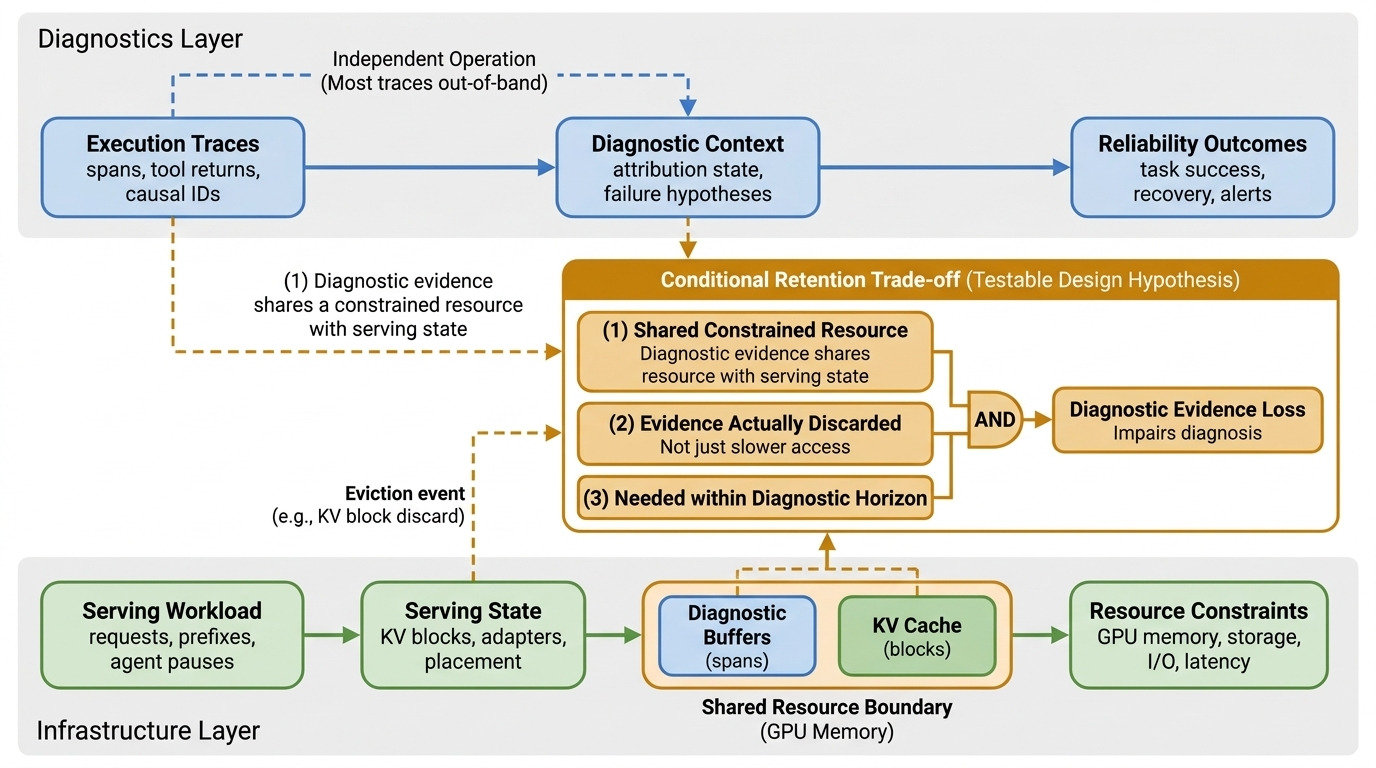
\includegraphics[width=0.94\linewidth,height=0.66\textheight,keepaspectratio]{figures/figure_1.jpg}
\caption{Bounded review scope. The diagnostics layer (top, blue) and infrastructure layer (bottom, green) manage different state objects. Dashed arrows indicate conditional cross-layer dependencies: diagnostic evidence loss requires all three conditions (shared constrained resource, evidence actually discarded, needed within the diagnostic horizon). Most traces are stored out-of-band and survive KV cache eviction.}\label{fig:v5_1}\end{figure}

\subsection{Positioning among recent surveys}
Recent surveys available online in Neurocomputing offer complementary perspectives on agent lifecycles, architecture and evaluation, graph-based coordination, embodied decision-making, and inference serving \cite{survey_lifecycle,survey_agentic,survey_graph,survey_embodied,survey_serving}. Li et al.~\cite{ext043} connect multi-agent workflows to supporting infrastructure at a broader level. Table~\ref{tab:v5_1} identifies where these perspectives inform the present review. Our unit of comparison is the execution artifact and the conditions under which it can support diagnosis after a serving decision.

\begin{table}[!htbp]
\centering
\small
\caption{Scope of related Neurocomputing surveys and the questions they motivate here.}
\label{tab:v5_1}
\begin{tabularx}{\linewidth}{@{}p{.26\linewidth}XX@{}}
\toprule
Survey & Organizing principle & Question for diagnostic and serving research \\
\midrule
Agent lifecycles \cite{survey_lifecycle} & Lifecycle stages and graph augmentation & Which artifacts connect evidence across stages? \\
Agentic AI systems \cite{survey_agentic} & Architecture, interaction, and evaluation & What evidence supports attribution at the agent or step level? \\
LLMs and graph neural networks \cite{survey_graph} & Coupling between language models and graph components & When do graph relations represent observed dependencies in an execution? \\
Embodied AI \cite{survey_embodied} & Hierarchical and end-to-end decision-making & Which external observations must be recorded because replay can change them? \\
Inference load balancing \cite{survey_serving} & Serving control and learning mechanisms & Which resource decisions affect access to diagnostic evidence? \\
\bottomrule
\end{tabularx}
\end{table}

\section{Background}
This section establishes the technical context for the diagnostic and infrastructure layers reviewed in subsequent sections. We describe the architecture of foundation model-based multiagent systems (\S{}2.1), the workload characteristics that distinguish multi-agent serving from single-model inference (\S{}2.2), and the runtime layers we focus on (\S{}2.3).


\subsection{Foundation Model-Based Multi-Agent Systems}
% Contextual sources now cited in the supporting body argument.
% Bibliographic records have not all been independently full-text audited.
\paragraph{Agent architectures, coordination, and the boundary of this survey.}
Agent architectures range from multi-agent conversation frameworks and collaborative environments to interactive generative simulations~\cite{ext065,ext066,ext067}.
Cognitive accounts, verbal feedback and embodied tool-use agents expose different ways to retain memory, observations and action histories~\cite{ext068,ext071}.
These foundations explain why agent execution traces must be distinguished from short-lived model serving state, but they are not direct evidence of a measured KV-retention effect~\cite{ext080,ext081}.

Existing surveys organize LLM multi-agent research around workflows, coordination, autonomy and collaboration mechanisms~\cite{ext035,ext043,ext045,ext046,ext076}.
Other reviews focus on software-engineering agents, social simulations, communication or goal-directed interactive tasks~\cite{ext077,ext078,ext079,ext096}.
The present review instead uses evidence capture, replayability, attribution granularity and serving-resource assumptions as its primary comparison axes~\cite{ext103,ext104,ext110,ext112}.




A foundation model-based agent operates in a perception--reasoning--action loop, using an LLM to process observations and execute actions such as tool invocations, code execution, and interagent communication. The underlying model workloads can also be multimodal: recent systems combine visual, audio, and clinical or platform metadata for domain-specific prediction and governance. A multi-agent system (MAS) comprises multiple such agents, as exemplified by MetaGPT, CAMEL, ChatDev, and Internet of Agents (IoA), operating within a shared environment or communicating to accomplish collective objectives. Recent multi-agent applications also span reinforcement-learning-enhanced collaborative reasoning and multimodal misinformation detection. MAST \cite{v5ref5} identifies 14 recurring failure patterns in such systems, motivating runtime diagnostics rather than evaluation only at the final task output. The rapid expansion of MAS into production deployments introduces operational demands that simple orchestration frameworks do not address: when an agent fails mid-workflow, which agent caused the failure? When a serving system evicts cached state, does this affect later diagnostic capability? When a safety guardrail intercepts an action, does the interception itself create a new failure mode? Three broad system properties recur across the literature: (1) distributed execution across multiple agents, which creates execution traces spanning agent boundaries and introduces coordination overhead; (2) inter-agent communication, which creates channels through which failures can propagate (FAMAS's spectrum analysis and TraceElephant's trace collection both exploit these channels for attribution); and (3) inter-agent memory sharing, where prompts, tools, and cached state may be reused across the system, creating shared state dependencies that affect both serving efficiency and diagnostic evidence availability.


\subsection{Multi-Agent Workload Characteristics}
% Contextual sources now cited in the supporting body argument.
% Bibliographic records have not all been independently full-text audited.
\paragraph{Interaction patterns, reasoning histories, and evaluation consequences.}
Multi-agent deliberation studies consider debate, cooperation, negotiation and exchange of intermediate messages~\cite{ext069,ext070,ext074,ext082,ext083}.
Adaptive team structures and communication-topology studies further vary who participates, which messages are shared, and how the solution process unfolds~\cite{ext084,ext085,ext086,ext087}.
These designs generate heterogeneous communication histories; a later diagnosis can require message-level provenance that aggregate task success does not preserve~\cite{ext095,ext105,ext108,ext115}.

Trajectory-level approaches cover search-structured reasoning, counterfactual rollouts and intermediate supervision~\cite{ext055,ext056,ext061}.
Agent memory surveys, self-collaboration and reflection mechanisms likewise differentiate remembered experiences from the active prompt and model state~\cite{ext092,ext093,ext094}.
We treat these as candidate sources of replay requirements and intermediate evidence, not as direct experimental results on diagnostic-retention policies~\cite{ext102,ext111,ext062}.

Long-running social simulations and goal-directed collaboration create interactions whose externally visible state may persist beyond one model request~\cite{ext088,ext089}.
Task hierarchies and institutional multi-agent representations add organizational constraints and dependencies to these histories~\cite{ext090,ext091}.
These application settings motivate evaluation beyond isolated model completions while remaining outside the core 60-item evidence census~\cite{ext109,ext143}.



Multi-agent workloads differ from single-model serving in three ways that directly affect memory placement, scheduling, and cache policy:


Sparse activation. Only a fraction of agents invoke the LLM at any moment: a 1,000-agent simulation may have fewer than 10 actively generating tokens. Under such workloads, keeping all agent state on the fastest memory tier can waste scarce accelerator memory. ScaleSim's invocation-distance metric quantifies the temporal gap before an agent's next call, enabling memory-tier demotion for inactive agents.


Invocation distance. Many workloads have structured activation patterns such as sequential queues, event-driven messaging, and dependency graphs. The temporal gap before an agent's next call, termed invocation distance, can be estimated from application semantics in structured workloads but is not generally visible to request-level schedulers. This motivates workflowaware caching approaches such as KVFlow, which predicts steps-to-execution for each cached prefix.


Inter-agent memory sharing. Agents may share context such as system prompts, environment descriptions, and tool schemas. General serving systems already reuse such prefixes: SGLang's RadixAttention and vLLM's automatic prefix caching both exploit shared token sequences. The additional opportunity in agentic systems is to use application-level structure (dependency graphs, message queues, or execution order) to guide cache retention decisions beyond request-level recency or frequency heuristics. The relative importance of these properties varies by application domain. Simulation workloads (ScaleSim's target) exhibit strong sparse activation with predictable invocation patterns. Coding agent workflows (Continuum's target) have long tool-call pauses with uncertain durations. Multi-model deployments (DroidSpeak's target) add cross-architecture cache transfer challenges. The infrastructure systems reviewed in Section 5 address different subsets of these workload properties, and the optimal KV-cache management strategy depends on which properties dominate in a given deployment.


\subsection{Runtime Layers}
% Contextual sources now cited in the supporting body argument.
% Bibliographic records have not all been independently full-text audited.
\paragraph{Operational interfaces, durable traces, and non-paper evidence.}
Agent-operations and infrastructure work distinguishes lifecycle management, workflow orchestration, operational tracing and the execution of a single model request~\cite{ext012,ext013,ext017,ext032,ext034,ext041,ext044}.
Durable-execution and tracing documentation describe engineering interfaces for storing process state and making actions observable~\cite{ext116,ext117,ext121,ext122,ext131,ext132}.
Protocol specifications, deployment guidance and commercial product documentation supply contextual implementation vocabulary but are not treated as peer-reviewed measurements of failure-attribution accuracy or cache costs~\cite{ext140,ext048,ext119,ext127,ext129,ext130}.



We focus on two runtime layers that are less mature than orchestration:


Diagnostics layer. This layer supports failure localization (identifying which agent or step caused a failure), observability and tracing (continuously capturing execution evidence), and safety intervention (actively monitoring and preventing harmful actions). The diagnostic layer consumes execution state --- traces, tool outputs, intermediate reasoning --- to produce reliability outcomes: attribution reports, anomaly alerts, and safety blocks. The surveyed methods vary dramatically in their resource requirements: FAMAS requires 20 environment replays averaging 105 minutes per task, while MASPrism requires only two deterministic prefill passes at 2.66 seconds on a 0.6B model. This three-orders-of-magnitude cost range has direct implications for cross-layer design: methods at the high end of the cost spectrum may compete with serving resources, while methods at the low end operate well within available headroom.


Infrastructure layer. This layer manages serving-time resources: KV-cache memory, compute scheduling, adapter placement, and power management for multi-agent workloads. The infrastructure layer consumes serving state --- KV blocks, adapters, request metadata --- and optimizes for throughput, latency, and resource utilization. Among the 22 Tier-1 infrastructure


systems surveyed, eviction mechanisms range from simple LRU (SGLang) to learned survivalbased predictions (the policy-driven runtime), with 8 systems incorporating agent-level metadata into their management decisions. The key distinction is between reactive eviction (triggered by memory pressure) and predictive eviction (triggered by estimated future reuse), with the latter providing more opportunity for diagnostic-aware retention. The distinctive question for this review is which state dependencies cross the diagnostic/serving boundary, and which apparent similarities between the two layers do not constitute resource competition. This question is formalized in Section 6.


% The extended source map is contextual; it does not change the 60-core census.
\section{Review Methodology}\label{sec:method}
We assembled a curated critical-review corpus through iterative database exploration, backward/forward citation chaining, and eligibility-based selection. Because database-specific search logs and screening decisions were not retained, we do not report a PRISMA-style numerical flow or claim systematic completeness. The PRISMA 2020 guidelines \cite{v5ref26} informed the reporting structure only. The sources, inclusion criteria, and final corpus composition are summarized in \ref{app:curated_flow} (Figure~\ref{fig:v5_corpus_flow}). We describe our search strategy, selection criteria, evidence-coding scheme, and the classification taxonomy below.


\subsection{Search Strategy}
We conducted iterative searches across five academic databases: IEEE Xplore, ACM Digital Library, Scopus, Google Scholar, and arXiv. The initial search window spanned January 2024 through March 2026, followed by a targeted citation-chaining update through August 2026, and a final update pass through November 2026 capturing systems announced at NeurIPS 2025, ICML 2026, ACL 2026, EMNLP 2026, OSDI 2024, FAST 2025, and EuroSys 2025/2027. Because foundation-model multi-agent runtime research is rapidly evolving, we included preprints alongside peer-reviewed publications when the described system contained reproducible implementation details. We prioritize work from 2024--2026 because foundation-model multi-agent runtime research is unusually recent, while retaining older serving papers when they define mechanisms directly reused by agentic systems. We constructed Boolean search queries combining terms from two domains:


$\bullet$ Diagnostics: (``multi-agent'' OR ``LLM agent'' OR ``foundation model agent'') AND (``failure localization'' OR ``fault attribution'' OR ``debugging'' OR ``observability'' OR ``tracing'' OR ``guardrail'' OR ``safety intervention'' OR ``runtime monitoring'') $\bullet$ Infrastructure: (``multi-agent'' OR ``LLM serving'' OR ``agent serving'') AND (``KV cache'' OR ``memory management'' OR ``scheduling'' OR ``state sharing'' OR ``cache eviction'' OR ``prefix caching'' OR ``context reuse'') Cross-domain queries additionally combined diagnostic and infrastructure terms to capture systems at the intersection (e.g., ``KV cache eviction'' AND ``diagnostic evidence''). To make the review more reproducible without overstating exhaustiveness, candidate papers were collected iteratively from primary systems papers, adjacent surveys, major peer-reviewed venues, and forward/backward citation tracing. Queries were adapted per database syntax. A paper enters the core system tables only when its runtime role can be identified from the source and mapped to one of the functions above. Because the corpus was not generated by a preregistered database protocol with fixed search strings and PRISMA-style screening, the reported counts should be interpreted as a curated landscape rather than an exhaustive census.


Citation chaining. After the initial query-based search, we performed forward citation tracing (finding papers that cite a seed paper) and backward citation tracing (examining references within each selected paper). This process identified 34 additional failure-localization systems not captured by the initial queries, primarily because they use domain-specific terminology (``root cause analysis,'' ``trajectory debugging,'' ``error attribution'') that does not always cooccur with ``multi-agent'' in titles or abstracts. We also traced infrastructure systems through the KV-cache-management citation network starting from vLLM and SGLang, identifying 16 additional systems that address multi-agent workload patterns.


\subsection{Inclusion and Exclusion Criteria}
Inclusion criteria. A paper enters the core system tables when it satisfies at least one of the following:


1. It describes a runtime diagnostic operation for foundation-model agents: failure localization, observability or tracing, safety intervention, or diagnostic benchmarking. 2. It describes a serving-time resource management mechanism (memory, scheduling, cache, or power) reused by or designed for agentic workloads. 3. It provides a baseline or architectural prerequisite directly reused by multi-agent diagnostic or serving systems.


Exclusion criteria. We exclude: (a) orchestration-only frameworks without runtime diagnostic or serving mechanisms (e.g., workflow graph definitions); (b) single-model inference optimization without multi-agent or agentic extensions; (c) offline-only evaluation methods that do not address runtime behavior; (d) long-term memory architectures without serving-time resource management; and (e) general agent surveys that do not provide system-level implementation details for diagnosis or serving.


Selection cutoff. The reference list was frozen for editorial inspection on 7 November 2026. This is a revision cutoff, not a systematically reconstructed search date: the original exploratory collection did not preserve database-by-database queries, retrieval timestamps, or screening exclusions. We therefore describe the corpus as a curated landscape rather than claiming PRISMA-style systematic completeness.


\subsection{Evidence Coding}
Each included system is assigned an evidence tier that reflects the depth of our verification:


$\bullet$ Tier 1a (T1a): Full-text reading with section-level evidence extraction. Quantitative claims, method details, cost metrics, and limitations are traced to specific sections, tables, or figures in the source paper. The core comparison tables contain both T1 and four explicitly labeled T2 entries; T2 claims require abstract-only limitations. $\bullet$ Tier 1b (T1b): Full-text reading but without page-level citation (e.g., the evidence was extracted from the complete paper but specific section numbers were not recorded). $\bullet$ Tier 2 (T2): Abstract-level verification. The system's existence, claimed function, and headline results are confirmed, but detailed method mechanics and cost breakdowns are not independently verified. Abstract-only evidence is marked [a] in the text and is not used to compute cross-system deltas or rankings. A source-level evidence-audit checklist accompanies the supplementary material.


\subsection{Classification Taxonomy}
We organize the reviewed systems along two orthogonal dimensions: function and method characteristics. This separation addresses a recurring classification ambiguity in the literature, where systems are categorized by their implementation strategy rather than the runtime role they serve.


Functional categories. We identify four primary functions in the diagnostic layer and three in the infrastructure layer: Diagnostic functions:


1. Localization: Identify which agent, step, or action caused a failure. 2. Monitoring: Continuously observe execution to detect anomalies or collect traces. 3. Intervention: Actively modify execution to prevent or recover from failures. 4. Evaluation: Assess system reliability, safety, or diagnostic quality post-hoc or online. Infrastructure functions:


1. State management: Retain, evict, or transfer cached computation state across requests. 2. Scheduling: Allocate compute, memory, or I/O resources across concurrent agent workloads. 3. Placement: Decide where to store or process agent-specific state across memory tiers or nodes.


Method dimensions. Within each functional category, we characterize systems along six dimensions that affect deployment feasibility and cross-layer interactions:


1. Evidence inputs: What execution data does the method consume? (e.g., full traces, toolcall logs, attention scores, prefill outputs) 2. Training requirements: Does the method require task-specific training, general pretraining, or no training? 3. Replay requirements: How many environment re-executions does the method need? (0, fixed k, or adaptive) 4. Attribution granularity: At what level does the method operate? (system, agent, step, action, token) 5. Intervention timing: Is the method post-hoc, online, or preemptive? 6. Runtime cost: What are the computational, memory, and latency overheads? A system may serve multiple functions (e.g., a guardrail that both monitors and intervenes) and may exhibit different cost profiles depending on its deployment mode. The comparison tables in Sections 4 and 5 record each system's primary function and characterize it along all six dimensions where evidence is available.


\subsection{Evidence Extraction Process}
For each Tier-1 system, we performed a structured extraction following a fixed template with 10 dimensions: (1) full citation with arXiv ID and venue; (2) state type managed (for infrastructure) or method category (for diagnostics); (3) eviction/retention policy mechanism or attribution approach; (4) runtime assumptions (model homogeneity, memory topology, multitenancy, workload pattern); (5) shared diagnostic-serving retention budget assessment (with explicit ``confirmed absent by exhaustive reading'' notation); (6) training and replay requirements with quantified costs; (7) cost metrics with section-level evidence locations; (8) main limitations (author-stated plus reviewer-identified); (9) evidence locations table mapping each


finding to its source section, table, or figure; and (10) cross-layer analysis notes assessing the system's relevance to the diagnostic-infrastructure interaction. This structured template ensures that the comparison tables in Sections 4 and 5 report consistent dimensions across all systems. The template was developed iteratively: the first five systems (SGLang, ScaleSim, DistServe, Mooncake, Parrot) were extracted using a preliminary template, and the template was refined based on which dimensions proved most informative for cross-system comparison. All subsequent extractions used the refined template. A verification step was applied to each extraction: quantitative claims in the extraction template were cross-checked against the source paper's tables and figures (not just the text). Several discrepancies were identified and corrected: for example, a preliminary extraction attributed 66\% accuracy to FAMAS, but the source paper's Table 2 shows 62.07\% as the best agent-level figure on handcrafted scenarios; similarly, TrajAudit's trajectory folding was initially recorded as 86--92\% but the source paper (\S{}VII-D) reports 94.6\%.


\subsection{Corpus Composition}
The core corpus contains 48 diagnostic and serving entries and 12 evaluation benchmarks (Appendix~\ref{app:census}). The 48 entries comprise 12 localization methods, 6 observability systems, 8 intervention and guardrail systems, and 22 serving systems. The source census records full-text assessment for 56 entries and abstract-level assessment for four localization methods (StepFinder, FALAT, DoVer, and VerifyMAS). We use the latter to map coverage and reserve detailed comparisons for sources with fuller evidence. Related surveys provide context for the review and fall outside the core census.

\section{Diagnostics}
This section organizes the diagnostic landscape along functional roles rather than implementation categories, following the taxonomy introduced in Section 3.4. We cover failure localization (\S{}4.1), observability and tracing (\S{}4.2), safety intervention and guardrails (\S{}4.3), and diagnostic benchmarks (\S{}4.4). For each subsection, methods are characterized along the six method dimensions defined in Section 3.4: evidence inputs, training requirements, replay demands, attribution granularity, intervention timing, and runtime cost. Figure~\ref{fig:v5_3} provides a matrix view of the taxonomy with representative systems placed in cells.


\subsection{Failure Localization}
% Contextual sources now cited in the supporting body argument.
% Bibliographic records have not all been independently full-text audited.
\paragraph{Localization, repair, provenance and verification beyond the core census.}
Adjacent failure-localization approaches study zero-replay diagnosis, hierarchical blame assignment, causal reasoning and diagnosis-guided repair~\cite{ext001,ext002,ext004}.
Interactive debugging and graph-guided intervention can require different visibility into state changes and different opportunities to replay an action~\cite{ext005,ext007}.
Because these source records span heterogeneous evaluation settings, we use them to refine mechanism categories rather than pooling their reported scores into a single accuracy ranking~\cite{ext037,ext114}.

Security-audit graph proposals and automated agent-auditor systems focus on making agent behavior inspectable~\cite{ext015,ext016}.
Online failure monitoring changes the observation and alarm timing relative to retrospective blame assignment~\cite{ext021}.
These differences imply different retention horizons, alert-denominator definitions and requirements for recording unrepeatable tool observations~\cite{ext053}.



Failure localization identifies which agent, step, or action caused an observed failure. We identify four methodological families among the 8 Tier-1 methods reviewed: statistical methods adapted from software fault localization, LLM-guided methods that use a language model as an investigator, RL-trained methods that learn attribution policies, and training-free signalextraction methods that exploit model internals.



% Figure 2 - faithful 4-by-6 diagnostic taxonomy matrix.
% Editable text; same row/column arrangement as original, enlarged by
% scaling the original vector matrix to portrait page text width.
\begin{figure}[!htbp]
\centering
\begingroup
\setlength{\tabcolsep}{3pt}
\renewcommand{\arraystretch}{1.0}
\definecolor{taxblue}{RGB}{203,226,248}
\definecolor{taxgreen}{RGB}{211,235,218}
\definecolor{taxyellow}{RGB}{255,241,200}
\newcommand{\taxtext}[2]{\cellcolor{#1}\parbox[c][2.12cm][c]{3.00cm}{\centering\fontsize{10.5}{12.6}\selectfont #2}}
\fontsize{10.5}{12.6}\selectfont
{\bfseries\Large Diagnostic Taxonomy Matrix}\par\bigskip
\resizebox{\linewidth}{!}{%
\begin{tabular}{@{}>{\raggedright\arraybackslash}p{2.67cm}|*{6}{>{\centering\arraybackslash}p{3.13cm}|}@{}}
& \textbf{Evidence inputs} & \textbf{Training required} & \textbf{Replay required} & \textbf{Attribution granularity} & \textbf{Intervention timing} & \textbf{Runtime cost type}\\
\cline{2-7}
\textbf{Localization} &
\taxtext{taxblue}{Traces, prefill signals, trajectories} &
\taxtext{taxyellow}{None (CHIEF, FAMAS); RL (AgenTracer)} &
\taxtext{taxyellow}{20$\times$ (FAMAS); 0 (others)} &
\taxtext{taxgreen}{Agent, step, action} &
\taxtext{taxgreen}{Post-hoc} &
\taxtext{taxblue}{Replay count, tokens, parameters}\\
\cline{2-7}
\textbf{Monitoring} &
\taxtext{taxblue}{Spans, logs, corpus traces} &
\taxtext{taxgreen}{None} &
\taxtext{taxgreen}{None} &
\taxtext{taxgreen}{Span/event level} &
\taxtext{taxgreen}{Online + offline} &
\taxtext{taxblue}{\$/run; ms overhead}\\
\cline{2-7}
\textbf{Intervention} &
\taxtext{taxblue}{Context, policy, graph structure} &
\taxtext{taxyellow}{GNN (G-Safe), SFT optional} &
\taxtext{taxgreen}{None} &
\taxtext{taxgreen}{Agent/message level} &
\taxtext{taxyellow}{Pre/post action} &
\taxtext{taxblue}{Latency (ms), API queries}\\
\cline{2-7}
\textbf{Evaluation} &
\taxtext{taxblue}{Labeled failures, traces} &
\taxtext{taxgreen}{None} &
\taxtext{taxyellow}{Varies} &
\taxtext{taxgreen}{Agent, step, failure mode} &
\taxtext{taxgreen}{Offline evaluation} &
\taxtext{taxblue}{Scale (\# traces), coverage}\\
\cline{2-7}
\end{tabular}%
}
\par\medskip
\caption{Functional diagnostic taxonomy. The original four roles, six method dimensions, cell content, and color coding are preserved; labels are re-typeset as searchable, enlarged LaTeX text. Role-level descriptions are representative, not universal requirements for each method.}
\label{fig:v5_3}
\endgroup
\end{figure}

\paragraph{Localization from repeated executions.}
FAMAS \cite{v5ref11} contrasts action patterns across runs using spectrum-based fault localization. Repeated executions provide variation that a static trace cannot supply, at the cost of reconstructing the environment and paying for additional runs. DoVer \cite{v5ref22} is an emerging intervention-based approach. The evidence available for this review supports its inclusion in the landscape, with limited basis for comparing operational cost or attribution accuracy.

\paragraph{Localization from recorded trajectories.}
CHIEF and TrajAudit structure a trajectory before using a language model to narrow the candidate failure region \cite{v5ref38,v5ref35}. CHIEF backtracks through dependencies between subtasks and agents, while RAFFLES searches for a failure location through iterative reasoning \cite{v5ref51}. AgentRx examines actions against mined constraints \cite{v5ref3}. These choices trade richer local context against the cost of analyzing long trajectories. A static record can support competing explanations when the agent's inputs, tool responses, or downstream effects are missing. Textual hypothesis verification, as explored by VerifyMAS \cite{v5ref31}, inherits this dependence on the trace.

\paragraph{Localization from learned or internal signals.}
AgenTracer and supervised verifiers adapt the diagnostic model to labeled trajectories or generated supervision \cite{v5ref45,v5ref40}. MASPrism instead extracts prefill-stage signals from an open-weight model \cite{v5ref19}. This lowers the need for task-specific training and introduces a different dependency: the evaluator must have access to model internals. StepFinder and FALAT are additional emerging approaches represented by limited evidence in the corpus \cite{v5ref52,v5ref33}.

\paragraph{What the comparisons establish.}
Table~\ref{tab:v5_2} compares input, training, replay, granularity, timing, and cost. A method evaluated only on known failures supports attribution after detection. Using it for online monitoring also requires evidence about false alarms and decision delay on successful runs. Likewise, agent-level and step-level attribution require different labels, and figures from separate benchmarks cannot establish a common ordering. TRAIL's span annotations illustrate the additional supervision needed to evaluate localization within a trace \cite{v5ref10}.

\subsection{Observability and Tracing}
% Contextual sources now cited in the supporting body argument.
% Bibliographic records have not all been independently full-text audited.
\paragraph{Provenance-oriented observability.}
AgentOps and AI-observability accounts emphasize event capture, process provenance and analysis across running agent workflows~\cite{ext008,ext009}.
Process mining provides a complementary model for reconstructing ordered operational events from retained execution records~\cite{ext011,ext014}.
Neither class of work by itself establishes that removing GPU-resident KV-cache blocks destroys separately persisted diagnostic traces; the storage dependency must be demonstrated~\cite{ext141}.




Observability systems continuously capture execution evidence during agent operation, providing the raw data that localization and safety methods consume. We identify three levels of maturity: conceptual taxonomies that define what should be traced, protocol-level standards that specify how traces are encoded, and tooling that implements the capture pipeline.


Conceptual taxonomies. The Agent Traces survey \cite{v5ref39} proposes a six-dimensional provenance taxonomy that structures the observability design space. The six dimensions are: (1) trace sources (instructions/inputs, reasoning, retrieval, tool use, MCP boundaries, memory, environment, multi-agent communication); (2) evidence and execution units (content-bearing artifacts vs. occurrences with actor and timestamp); (3) provenance relations (nine relations in four families: semantic support, content derivation, causal dependence, and procedural dependence); (4) tracing granularity and timing (run, step, tool-call, parameter, claim, and token/span levels; pre-execution, runtime, post-hoc, continuous); (5) representation forms (structured logs, execution graphs, evidence graphs, provenance graphs, runtime state); and (6) trust functions


\begin{table}[!tbp]
\centering
\caption{Multi-axis comparison of failure-localization methods. Panels A and B show complementary dimensions for the same twelve methods. NR denotes not reported; precise T2 details require independent full-text verification.}
\label{tab:v5_2}
\begingroup
\setlength{\tabcolsep}{3pt}
\renewcommand{\arraystretch}{1.14}
\footnotesize
\noindent\textbf{Panel A. Evidence and execution requirements}\par\smallskip
\begin{tabular}{@{}Y{.16\linewidth}Y{.205\linewidth}Y{.267\linewidth}Y{.185\linewidth}Y{.099\linewidth}@{}}
\toprule
\textbf{Method} & \textbf{Category} & \textbf{Evidence input} & \textbf{Training} & \textbf{Replays} \\
\midrule
FAMAS & Statistical & Re-executions & No & 20 \\
TrajAudit & LLM guided & Trajectories & No & 0 \\
AgenTracer & RL trained & Failure traces & RL, 8B & 0 \\
MASPrism & Signal extraction & Prefill NLL & No & 0 \\
CHIEF & LLM guided & Causal graph & No & 0 \\
AgentRx & LLM guided & Traces+schemas & No & 0 \\
RAFFLES & LLM guided & Execution traces & No & 0 \\
Xia et al. & Supervised & Traces+verification & LoRA & 0 \\
StepFinder & Supervised & Temporal features & BiLSTM & 0 \\
FALAT & LLM guided & Dependencies & No & 0 \\
DoVer & Intervention & Snapshots & No & 4--12* \\
VerifyMAS & LLM guided & Hypotheses+NLI & Optional SFT & 0 \\
\bottomrule
\end{tabular}
\par\medskip
\noindent\textbf{Panel B. Resource profile and output granularity}\par\smallskip
\begin{tabular}{@{}Y{.226\linewidth}Y{.154\linewidth}Y{.156\linewidth}Y{.287\linewidth}Y{.096\linewidth}@{}}
\toprule
\textbf{Method} & \textbf{Tokens} & \textbf{Model} & \textbf{Granularity} & \textbf{Tier} \\
\midrule
FAMAS & NR & 72B & Action & T1a \\
TrajAudit & 138K & Frontier & Step & T1a \\
AgenTracer & NR & 8B & Agent + Step & T1b \\
MASPrism & 7K & 0.6B & Step & T1a \\
CHIEF & 55K & 671B & Agent + Step & T1a \\
AgentRx & 5--16K & Frontier & Step & T1a \\
RAFFLES & NR & NR & Step & T1a \\
Xia et al. & NR & NR & Agent & T1b \\
StepFinder & NR & NR & Step & T2 \\
FALAT & NR & NR & Step & T2 \\
DoVer & NR & NR & Step / Recovery & T2 \\
VerifyMAS & NR & NR & Agent + Error & T2 \\
\bottomrule
\end{tabular}
\par\smallskip\raggedright\scriptsize *Reported at T2 evidence depth; replay count not independently full-text audited.
\endgroup
\end{table}
(verification, attribution, debugging, safety enforcement, audit, recovery). Two cross-cutting attributes qualify every relation: provenance origin (instrumented, inferred, declared, or derived) and trace assurance (logged, tamper-evident, or attested), with attested being ``the least developed attribute in the works reviewed'' (\S{}2.2). The survey catalogs 27 representative systems (Table 3), 25 benchmarks (Table 8), 20 guardrail systems (Table 5), and 11 memory systems (Table 6). A key architectural insight is the distinction between evidence units (content-bearing artifacts such as tool outputs) and execution units (occurrences with actor and timestamp), which determines whether a trace record is sufficient for post-hoc attribution. Three gaps are identified: limited integration of fine-grained provenance with trust functions, no benchmark evaluating complete provenance chains, and insufficient tamper-evident reporting.


Protocol-level standards. The OpenTelemetry GenAI semantic conventions \cite{v5ref25} provide vendorneutral attributes for LLM inference spans. Core gen\_ai.* attributes include operation name (chat, embeddings, execute\_tool, create\_agent, invoke\_agent, invoke\_workflow), provider and model identity, input/output token counts, cache read/creation tokens (v1.40), reasoning output tokens for chain-of-thought models (v1.41), streaming flags and TTFT (v1.41), and agent/tool identifiers. MCP-specific attributes (mcp.method.name, mcp.session.id, mcp.protocol.version) were added in v1.39. Content events (prompts, completions, system instructions) are opt-in, controlled by an environment flag for privacy. Proposed agentic extensions (Issue \#35: task, action, team, artifact, and memory attributes) remain in ``Todo'' status as of November 2026. The specification remains at Development status with no stabilization timeline, and provider coverage is uneven: OpenAI instrumentation is the most complete, while Anthropic, AWS Bedrock, and Google Vertex AI libraries have less detailed support. Framework-level integration for LangGraph and CrewAI is in progress but incomplete. A fundamental architectural limitation is that OTel captures telemetry about model calls but provides no enforcement capability: ``telemetry can't answer enforcement questions.'' For cross-layer analysis, the most significant gap is the absence of serving-side attributes (cache residency, eviction events, memory pressure, adapter loading status) that would enable correlating diagnostic trace availability with infrastructure state.


Tooling. AgentTrace \cite{v5ref2} implements three logging surfaces --- operational (method-level execution tracing with paired start/complete events), cognitive (LLM reasoning chain extraction including CoT parsing, confidence estimates, and plan/reflection fields), and contextual (outbound API interactions auto-instrumented via OTel monkey-patching) --- unified under a schema-validated append-only envelope with UUID, surface type, trace/span IDs, and UTC timestamps (\S{}3.1--3.6). The system produces dual output: JSONL files for local analysis and OTel spans for distributed backends. While the architecture is well-specified with pseudocode (Algorithm 1, \S{}4.2), no empirical evaluation of overhead, latency, or storage costs is reported (\S{}4.5 states only ``low overhead'' qualitatively). No repository link or package name is provided. Insights Generator \cite{v5ref23} provides analytics over collected execution traces, enabling aggregate analysis across multiple agent runs: failure frequency by step type, time-to-failure distributions, and cross-agent correlation patterns. The view-oriented debugging compiler \cite{v5ref46} transforms raw execution logs into interactive visual representations: the compiler applies view transformations (filtering, aggregation, temporal alignment) to produce domain-specific debugging views from a common trace format, enabling human inspectors to navigate complex multiagent executions without manually parsing log files. LangSmith (LangChain, commercial tooling) documents a trace collection and analysis platform with LLM evaluation features~\cite{v5supp1}; its proprietary nature limits independent verification of overhead and accuracy claims. The observability layer's principal limitation for cross-layer analysis is coverage: no existing standard captures the serving-side state (KV cache residency, eviction events, memory pressure) that Section 6 identifies as relevant for diagnostic-infrastructure interaction. Extending OTel GenAI conventions to include serving-side attributes is one of the open directions proposed in Section 7.


\subsection{Safety Intervention and Guardrails}
% Contextual sources now cited in the supporting body argument.
% Bibliographic records have not all been independently full-text audited.
\paragraph{Threat surfaces, intervention timing and audit requirements.}
Surveys and guardrail designs separate preventive policy checks, runtime monitoring and post-hoc intervention~\cite{ext018,ext019,ext020,ext022}.
Communication attacks and prompt-infection work illustrate that malicious instructions can flow through messages and agent-to-agent tool interaction~\cite{ext033,ext054,ext075}.
An auditable safety mechanism must expose the action, triggering context and decision time; documentation alone does not prove its efficacy on a specific threat model~\cite{ext106,ext107,ext118}.

Tool and inter-agent communication protocols define interfaces for messages, capabilities and identity handling~\cite{ext120,ext123,ext124,ext125}.
Institutional and normative multi-agent work addresses complementary governance requirements and permitted actions~\cite{ext126,ext128,ext142}.
These resources provide deployment and accountability context, not empirical evidence for a direct causal relationship between serving-cache eviction and lost diagnostic evidence~\cite{ext144,ext145,ext146}.




Safety systems actively monitor and intervene in agent execution to prevent harmful actions. We review eight Tier-1 systems spanning three architectural patterns: graph-based guardrails, modular safety agents, and control-theoretic recovery.


Graph-based guardrails. G-Safeguard \cite{v5ref37} addresses a specific threat model: adversarial agents embedded within a multi-agent system that manipulate other agents through malicious utterances. The system constructs a multi-agent utterance graph from inter-agent communication, using SentenceBERT/MiniLM embeddings as node features and a learnable permutationinvariant fusion of interaction histories as edge features. An edge-featured GNN with a soft probabilistic classifier detects attacker nodes after each dialogue round. Trained on 800 samples from a GPT-4o-mini-based 8-agent MAS, the system scales to 20--80 agents without retraining. A key limitation is that detection is reactive: ``by the time G-Safeguard identifies an attacker, certain nodes within the MAS have already been successfully compromised.'' The system operates purely on the utterance graph and does not inspect internal model serving state (ACL 2025 Long Papers).


Modular safety agents. ShieldAgent \cite{v5ref8} represents safety policies as Linear Temporal Logic (LTL) formulas organized into action-based probabilistic rule circuits via Markov Logic Networks. For each agent action, the system extracts action/state predicates from policy documents, applies spectral clustering on state predicates for rule grouping, and evaluates via two finetuned guardrail models on InternVL2-2B. The Autonomous Safety Policy Manager (ASPM)


optimization reduces the number of predicates by 50--65\% and rules by 50--76\%, enabling efficient runtime verification. The system uses short-term memory (KV-cache, discarded after verification) and long-term memory (successful workflows, permanently stored), and is built on the MCP framework (ICML 2025). LlamaFirewall \cite{v5ref9} implements a three-layer defense architecture with distinct models per layer. PromptGuard 2 classifies input prompts for jailbreak/injection using energy-based loss with hardened tokenization, available in 86M-parameter (mDeBERTa-base) and 22M-parameter (DeBERTa-xsmall) variants. AlignmentCheck evaluates each agent action against the user's stated goal using the execution trace and selected action via few-shot prompting (no fine-tuning; Llama 4 Maverick recommended as backing LLM). CodeShield performs two-tiered code scanning: Semgrep rules plus regex patterns covering 50+ CWEs across 7--8 programming languages. The three layers have different timing: PromptGuard is preventive (pre-processing), AlignmentCheck is reactive (post-action), and CodeShield is reactive (pre-execution). The system is open-source.


Control-theoretic recovery. ReGuard \cite{v5ref29} applies control-theoretic principles to agent recovery: when a safety violation is detected, the system computes a corrective action using a formal model of the agent's state transition dynamics, rather than simply blocking the action. This enables graceful degradation rather than hard stops, but requires a tractable state model.


Additional safety systems. SAIGuard \cite{v5ref34} implements proactive defense via communicationstate simulation: it constructs an interaction graph over the MAS, encodes messages with Qwen3-Embedding-0.6B (2-layer GNN, 1024 hidden dimensions), and estimates the impact of incoming messages on local and global agent states. Risky messages are detected via reconstruction deviations from benign patterns and sanitized before propagation --- making SAIGuard the only preventive safety system in the survey. It reduces attack success rate from 16.51\% to 5.37\% (67.47\% reduction) while maintaining 89.83\% task accuracy and 98.68\% detection F1. A ``systemic risk amplification'' finding is notable: aggregated multi-agent attack success (51.78\%) far exceeds per-agent vulnerability (3.00\%). SentinelAgent \cite{v5ref12} implements three-level anomaly detection: node-level (individual agent behavior), edge-level (inter-agent communication anomalies), and path-level (multi-hop execution chain attacks). Path-level detection catches all 6 tested scenarios but has the highest compute cost. The system uses IBM Granite Guardian 3.2 and LlamaFirewall as pre-trained backends without custom training. Evaluation is qualitative only (2 case studies). AGrail \cite{v5ref21} provides a lifelong agent guardrail framework combining rule-based constraints with learned safety policies. The ``lifelong'' aspect enables policy updates as agents encounter new scenarios without retraining. AgentDoG 1.5 \cite{v5ref18} uses anomaly detection on execution patterns to identify both safety violations and performance degradation simultaneously --- the only system producing both a safety verdict and a diagnostic attribution from the same analysis. ReGuard \cite{v5ref29} applies control-theoretic recovery: when a safety violation is detected, it models state transition dynamics and computes a corrective action rather than simply blocking the agent. This enables graceful degradation but requires a tractable state model.


Diagnostic-safety overlap. Safety systems and diagnostic systems share a key requirement: both need access to the agent's execution state (tool calls, outputs, and intermediate reasoning). Three of the eight safety systems (SentinelAgent, AGrail, AgentDoG) explicitly consume diagnostic traces as input to their safety decisions. This overlap suggests that serving-side state


management --- particularly KV cache eviction policies --- can affect safety system effectiveness when it removes state that safety monitors depend on. Section~\ref{sec:retention} discusses when these dependencies matter.


\subsection{Benchmarks}
% Contextual sources now cited in the supporting body argument.
% Bibliographic records have not all been independently full-text audited.
\paragraph{Evaluation environments, native labels and reliability.}
Meta-evaluation and benchmarking surveys emphasize the dependence of an agent score on task definition, judge, sampling protocol and failure semantics~\cite{ext003,ext006,ext029}.
Benchmark auditing and unified evaluation efforts make explicit the difference between task completion, robustness, blame attribution and failure reporting~\cite{ext030,ext031,ext036}.
Therefore this review's capability matrix recognizes a native decisive-step label only when the benchmark's own annotation protocol provides it~\cite{ext038,ext039,ext139}.

General-agent and collaboration benchmarks measure performance across diverse cooperation and tool-use settings~\cite{ext072,ext073,ext133}.
Web, enterprise, desktop and software-repository environments provide more specific tasks and stateful interaction requirements~\cite{ext134,ext135,ext136}.
These tasks can generate useful traces, but end-state task success cannot substitute for independently labeled agent-level or step-level causes~\cite{ext137,ext138}.

Post-failure reporting and agent-as-a-judge evaluation introduce complementary ways to assess explanation quality and agent behavior~\cite{ext063}.
However, plausible narrative explanations and automatic judge ratings are not automatically equivalent to a verified causal failure step~\cite{ext101}.
Separate reporting and attribution metrics are therefore needed when selecting benchmarks for diagnostic experiments.


Following the practice of aligning benchmark targets with levels of capability \cite{survey_humor}, we group evaluations by the claim their labels support. Outcome benchmarks test whether the task reached a target state. Safety evaluations test whether actions violate a policy or whether a monitor intervenes. Attribution benchmarks ask where the decisive failure occurred. These outcomes require different labels, even when they are extracted from the same workflow.

\paragraph{Outcome and safety.}
Task-success and repeated-run metrics, such as those used by $\tau$-bench \cite{v5ref42}, can reveal brittle behavior without recording its origin. Safety tests can isolate unsafe actions, but an unsafe action label does not by itself identify the upstream decision that caused it. Table~\ref{tab:v5_3} distinguishes these capabilities from native causal annotations.

\paragraph{Attribution and evidence resolution.}
Who\&When and TraceElephant provide agent- and step-level annotations \cite{v5ref48,v5ref6}. RootSE provides step-oriented cases, while TRAIL evaluates localization within instrumented spans \cite{v5ref35,v5ref10}. These annotations support distinct units of analysis. A method can identify the agent associated with failure while failing to locate the decisive action or explain how the failure propagated. Meaningful comparisons require agreement on what counts as the decisive event and how earlier contributing events are treated.

\paragraph{Cross-layer coverage.}
Figure~\ref{fig:v5_4} maps the coverage of the twelve benchmarks in the core corpus. None provides matched diagnostic and serving measurements under controlled retention policies. A benchmark for this gap needs both annotated workflow events and serving events linked to the same execution.

% Source-coded matrix with much larger searchable XeLaTeX text.
% Two panels keep all 12 x 10 labels, rather than squeezing into raster art.
\begin{figure}[p]
\centering
\caption{Benchmark capability matrix: native attribution labels versus task outcomes. The same 12 benchmarks and ten axes as the V5 evidence matrix are preserved in two readable panels.}
\label{fig:v5_4}
\begingroup
\fontsize{9.2}{11.1}\selectfont
\setlength{\tabcolsep}{2.7pt}
\renewcommand{\arraystretch}{1.08}
\noindent\textbf{Panel A. Diagnostic and safety dimensions}\par\smallskip
\begin{tabularx}{\textwidth}{@{}>{\raggedright\arraybackslash}p{.229\textwidth}*{5}{>{\centering\arraybackslash}X}@{}}
\toprule
\textbf{Benchmark} & \textbf{Multi-agent} & \textbf{Native step RCA} & \textbf{Native agent RCA} & \textbf{Failure taxonomy} & \textbf{Safety eval.} \\
midrule
\textbf{TraceElephant} & \cellcolor{green!17}Yes & \cellcolor{green!17}Yes & \cellcolor{green!17}Yes & \cellcolor{yellow!23}Partial & \cellcolor{red!11}NR \\
\textbf{Who\&When} & \cellcolor{green!17}Yes & \cellcolor{green!17}Yes & \cellcolor{green!17}Yes & \cellcolor{yellow!23}Partial & \cellcolor{red!11}NR \\
\textbf{RootSE} & \cellcolor{red!11}NR & \cellcolor{green!17}Yes & \cellcolor{red!11}NR & \cellcolor{yellow!23}Partial & \cellcolor{red!11}NR \\
\textbf{$\tau$-bench} & \cellcolor{red!11}NR & \cellcolor{red!11}NR & \cellcolor{red!11}NR & \cellcolor{red!11}NR & \cellcolor{red!11}NR \\
\textbf{MultiAgentBench} & \cellcolor{green!17}Yes & \cellcolor{red!11}NR & \cellcolor{red!11}NR & \cellcolor{red!11}NR & \cellcolor{red!11}NR \\
\textbf{GuardianAgentBench} & \cellcolor{green!17}Yes & \cellcolor{red!11}NR & \cellcolor{red!11}NR & \cellcolor{yellow!23}Partial & \cellcolor{green!17}Yes \\
\textbf{ReliabilityBench} & \cellcolor{red!11}NR & \cellcolor{red!11}NR & \cellcolor{red!11}NR & \cellcolor{yellow!23}Partial & \cellcolor{red!11}NR \\
\textbf{Agent-SafetyBench} & \cellcolor{red!11}NR & \cellcolor{red!11}NR & \cellcolor{red!11}NR & \cellcolor{yellow!23}Partial & \cellcolor{green!17}Yes \\
\textbf{AgentHarm} & \cellcolor{red!11}NR & \cellcolor{red!11}NR & \cellcolor{red!11}NR & \cellcolor{red!11}NR & \cellcolor{green!17}Yes \\
\textbf{TAMAS} & \cellcolor{green!17}Yes & \cellcolor{red!11}NR & \cellcolor{red!11}NR & \cellcolor{yellow!23}Partial & \cellcolor{green!17}Yes \\
\textbf{ASB} & \cellcolor{red!11}NR & \cellcolor{red!11}NR & \cellcolor{red!11}NR & \cellcolor{yellow!23}Partial & \cellcolor{green!17}Yes \\
\textbf{OSGuard} & \cellcolor{yellow!23}Partial & \cellcolor{red!11}NR & \cellcolor{red!11}NR & \cellcolor{yellow!23}Partial & \cellcolor{green!17}Yes \\
ottomrule
end{tabularx}
parmedskip

oindent	extbf{Panel B. Robustness, interaction and availability}parsmallskip
egin{tabularx}{	extwidth}{@{}>{
aggedrightarraybackslash}p{.229	extwidth}*{5}{>{centeringarraybackslash}X}@{}}
	oprule
\textbf{Benchmark} & \textbf{Adversarial robustness} & \textbf{Collaboration} & \textbf{Fault reliability} & \textbf{Diag./infra. interaction} & \textbf{Public data} \\
midrule
\textbf{TraceElephant} & \cellcolor{red!11}NR & \cellcolor{yellow!23}Partial & \cellcolor{green!17}Yes & \cellcolor{red!11}NR & \cellcolor{green!17}Yes \\
\textbf{Who\&When} & \cellcolor{red!11}NR & \cellcolor{yellow!23}Partial & \cellcolor{red!11}NR & \cellcolor{red!11}NR & \cellcolor{green!17}Yes \\
\textbf{RootSE} & \cellcolor{red!11}NR & \cellcolor{red!11}NR & \cellcolor{green!17}Yes & \cellcolor{red!11}NR & \cellcolor{green!17}Yes \\
\textbf{$\tau$-bench} & \cellcolor{red!11}NR & \cellcolor{red!11}NR & \cellcolor{yellow!23}Partial & \cellcolor{red!11}NR & \cellcolor{green!17}Yes \\
\textbf{MultiAgentBench} & \cellcolor{red!11}NR & \cellcolor{green!17}Yes & \cellcolor{red!11}NR & \cellcolor{red!11}NR & \cellcolor{green!17}Yes \\
\textbf{GuardianAgentBench} & \cellcolor{red!11}NR & \cellcolor{yellow!23}Partial & \cellcolor{yellow!23}Partial & \cellcolor{red!11}NR & \cellcolor{yellow!23}Partial \\
\textbf{ReliabilityBench} & \cellcolor{red!11}NR & \cellcolor{red!11}NR & \cellcolor{green!17}Yes & \cellcolor{red!11}NR & \cellcolor{yellow!23}Partial \\
\textbf{Agent-SafetyBench} & \cellcolor{red!11}NR & \cellcolor{red!11}NR & \cellcolor{red!11}NR & \cellcolor{red!11}NR & \cellcolor{green!17}Yes \\
\textbf{AgentHarm} & \cellcolor{yellow!23}Partial & \cellcolor{red!11}NR & \cellcolor{red!11}NR & \cellcolor{red!11}NR & \cellcolor{green!17}Yes \\
\textbf{TAMAS} & \cellcolor{green!17}Yes & \cellcolor{red!11}NR & \cellcolor{red!11}NR & \cellcolor{red!11}NR & \cellcolor{green!17}Yes \\
\textbf{ASB} & \cellcolor{green!17}Yes & \cellcolor{red!11}NR & \cellcolor{red!11}NR & \cellcolor{red!11}NR & \cellcolor{green!17}Yes \\
\textbf{OSGuard} & \cellcolor{red!11}NR & \cellcolor{red!11}NR & \cellcolor{red!11}NR & \cellcolor{red!11}NR & \cellcolor{yellow!23}Partial \\
ottomrule
end{tabularx}
parsmallskip

oindent{ootnotesize Green = source-coded support; yellow = partial; pale red = NR/no verified native label. A task-success score is not a ground-truth agent or decisive-step attribution label. NR is not evidence of impossibility.}
endgroup
end{figure}

\begin{table}[!tbp]
\centering
\caption{Diagnostic and safety benchmarks. Attribution support means \emph{native} agent- or step-level root-cause labels, not task success or post-hoc interpretability. In particular, $\tau$-bench does not provide native step-level causal-attribution labels.}
\label{tab:v5_3}
\begingroup
\setlength{\tabcolsep}{3pt}
\renewcommand{\arraystretch}{1.16}
\footnotesize
\begin{tabular}{@{}Y{.250\linewidth}Y{.111\linewidth}Y{.154\linewidth}Y{.065\linewidth}Y{.247\linewidth}Y{.057\linewidth}@{}}
\toprule
\textbf{Benchmark} & \textbf{Venue} & \textbf{Scale (reported)} & \textbf{MAS} & \textbf{Native attribution} & \textbf{Tier} \\
\midrule
TraceElephant & ACL 2026 & 220 failures & Yes & Agent+Step & T1 \\
Who\&When & ICML 2025 & 184 failures & Yes & Agent+Step & T1 \\
RootSE & Preprint & 102 cases & No & Step & T1 \\
tau-bench & arXiv 2024 & NR & No & None (goal-state success) & T1 \\
MultiAgentBench \cite{v5supp7} & ACL 2025 & 600 tasks & Yes & No native RCA & T1 \\
GuardianAgent\newline Bench \cite{v5supp8} & Preprint & 580 scenarios & Yes & No verified step-RCA & T1 \\
ReliabilityBench \cite{v5supp9} & Preprint & 1,280 episodes & No & No native RCA & T1 \\
Agent-SafetyBench \cite{v5supp10} & Preprint & 2,000 & No & No native RCA & T1 \\
AgentHarm \cite{v5supp11} & ICLR 2025 & 440 tasks & No & No native RCA & T1 \\
TAMAS \cite{v5supp12} & ACL 2026 & 300 instances & Yes & No native RCA & T1 \\
ASB \cite{v5supp13} & ICLR 2025 & 10 scenarios & No & No native RCA & T1 \\
OSGuard \cite{v5supp14} & Preprint & 324 examples & No & Unsafe-action labels, not RCA & T1 \\
\bottomrule
\end{tabular}
\endgroup
\end{table}
\section{Serving Infrastructure}
This section reviews 22 Tier-1 infrastructure systems that manage serving-time state for LLMbased workloads, with emphasis on those designed for or directly applicable to multi-agent scenarios. We organize the analysis around three state-sharing categories that reviewers and practitioners often conflate: textual context sharing (\S{}5.1), exact KV-cache reuse (\S{}5.2), and cross-model cache transfer (\S{}5.3). Section 5.4 covers agent-specific extensions that bridge general-purpose serving toward multi-agent workloads.


\subsection{Textual Context Sharing}
Textual context sharing refers to systems that pass natural-language prompts, tool outputs, or conversation histories between agents or requests without sharing the underlying KV-cache tensors. Each recipient independently computes its own KV cache from the shared text. Parrot \cite{v5ref17} introduces semantic variables --- placeholder tokens that represent data dependencies between LLM API calls in a multi-step pipeline. The runtime constructs a directed acyclic graph (DAG) per session with requests as nodes and semantic variables as edges (\S{}4.2), enabling three optimizations. First, a PrefixHash mechanism detects sharing opportunities by hashing prompt prefixes bound through semantic variables. Second, an application-centric scheduler deduces per-request performance objectives (latency vs. throughput) from the DAG structure (\S{}5.2, Algorithm 1). Third, a custom GPU kernel combines FlashAttention and PagedAttention to minimize redundant memory loading for shared prefixes (\S{}5.3). Importantly, Parrot does not transfer computed KV blocks between requests; it coordinates scheduling so that shared prefixes are processed together, then explicitly frees the cache via FreeContext calls under continuous batching. The system achieves up to 11.7$\times$ latency improvement on MetaGPT multi-agent workloads (Figure 18a), and sustains 12$\times$ higher request rates on multi-tenant GPTs workloads (Figure 17). Token redundancy measurements across applications range from 3\% to 99\% (Table 1), confirming that textual prefix sharing is pervasive in agentic pipelines. A principal limitation is that Parrot's centralized manager may become a scalability bottleneck, and


dynamic control flow (conditional branches, native function calls) must still execute client-side (\S{}6, OSDI 2024). DistServe \cite{v5ref50} disaggregates prefill and decoding into separate GPU pools connected via pull-based RDMA, allowing each phase to be independently parallelized and scaled. For a 66Bparameter model with 512-token requests, each request's KV cache is approximately 1.13 GB (\S{}3.3), making transfer cost a first-class design concern. The key architectural insight is that prefill (compute-bound) and decoding (memory-bandwidth-bound) have complementary resource profiles, so co-locating them on the same GPU pool wastes resources in both directions. By disaggregating, DistServe achieves 2$\times$ goodput improvement on Llama-70B under SLA constraints (\S{}5). However, the KV transfer mechanism is intra-request (prefill-to-decode handoff within a single user's generation), not inter-agent sharing. No eviction policy is described; KV state is consumed and released per-request (OSDI 2024). For multi-agent scenarios, DistServe's disaggregation could be composed with inter-request prefix sharing (as SGLang or Mooncake provide), but no such composition has been evaluated.


\subsection{Exact KV-Cache Reuse}
% Contextual sources now cited in the supporting body argument.
% Bibliographic records have not all been independently full-text audited.
\paragraph{Serving-system comparators and the scope of shared-resource claims.}
Foundational LLM serving research explores request scheduling, prefix placement, memory limits and separating prefill from decoding~\cite{ext040,ext042,ext049,ext050}.
Attention implementations and inference engines change which computations and states are expensive to repeat~\cite{ext149,ext150,ext151}.
Serving performance improvements are relevant to the cost dimension of DRICE but cannot be read as demonstrated gains in causal agent-attribution accuracy~\cite{ext152,ext147,ext148}.

Agent-aware cache proposals and memory-management surveys consider resumed workflows, persistent state and cache-replacement trade-offs~\cite{ext025,ext026,ext027}.
Multi-adapter serving and admission-control work adds heterogeneity in tenancy, request scheduling and runtime policy constraints~\cite{ext028,ext051}.
To claim a diagnostic effect, such systems must be evaluated with an explicitly shared resource budget and a matched trace-fidelity measure~\cite{ext052,ext064}.




Exact KV-cache reuse retains computed attention tensors across requests that share identical token prefixes, avoiding redundant prefill computation. This is the dominant category among surveyed systems.


Foundation: PagedAttention. vLLM \cite{v5ref14} introduced PagedAttention, managing KV cache in non-contiguous fixed-size blocks with a page table. It uses all-or-nothing eviction when GPU memory is exhausted, preempting entire sequences rather than individual blocks. This establishes the baseline architecture that most subsequent systems extend.


Prefix-tree indexing. SGLang \cite{v5ref49} organizes cached KV prefixes in a radix tree with LRU leaf-first eviction and reference counting. Each node maintains a reference counter; a node is evictable only when its counter reaches zero (\S{}3). Evicting leaves first enables reuse of common ancestors until those ancestors themselves become leaves. A key design decision is the dynamic shared pool: there is no fixed cache budget --- ``we do not preallocate a fixed-size memory pool as a cache; instead, we let the cached tokens and the currently running requests share the same memory pool'' (\S{}3). When enough waiting requests exist, the system evicts all cached tokens in favor of a larger batch size, prioritizing throughput over cache hit rate. Cache-aware scheduling sorts requests by matched prefix length; Theorem 3.1 proves this achieves optimal cache hit rate equivalent to DFS order on the radix tree. On Chatbot Arena workloads, SGLang achieves 52.4\% cache hit rate on LLaVA-NeXT-34B and 74.1\% on Vicuna-33B, with 1.7$\times$ TTFT reduction (\S{}5.5). Across benchmarks, it delivers up to 6.4$\times$ throughput improvement and 3.7$\times$ latency reduction over baselines including Guidance v0.1.8 and vLLM v0.2.5 (\S{}5). The overhead of RadixAttention itself is under 0.3\% of total inference time (\S{}5). For our cross-layer analysis, two properties of SGLang are noteworthy. First, the radix tree stores only KV tensors --- no adapter weights, LoRA parameters, or diagnostic state are managed (\S{}3). The system is single-model per instance, with no multi-adapter or multi-tenant cache partitioning. Second, the ``evict all cached tokens'' pressure response is the most aggressive eviction policy among surveyed systems: when memory pressure is high enough, the entire diagnostic-irrelevant cache is cleared. This design is optimal for request-level throughput but would need modification to protect diagnostically valuable prefixes. Stated limitations include


starvation under greedy scheduling (\S{}8), restriction to a single memory tier (GPU only; extending to CPU/disk is future work), and exact-match-only prefix lookup (no fuzzy or semantic matching).


Cost-benefit eviction. Mooncake \cite{v5ref32} disaggregates KV cache from compute into a distributed cache pool called KVCache Pool, accessed via one-sided RDMA reads that bypass the serving engine's critical path. The architecture separates prefill nodes (which generate KV blocks) from decode nodes (which consume them), with cache blocks stored on dedicated cache nodes. Mooncake implements configurable eviction policies (LRU, LFU, or hybrid) with a costbenefit model that weighs cache retention value against RDMA transfer bandwidth. Under a prefix-heavy workload, Mooncake achieves up to 525\% throughput improvement while maintaining latency SLAs. The system received the FAST 2025 Best Paper Award. For multi-agent scenarios, Mooncake's disaggregated architecture decouples cache lifetime from compute lifetime: a cached prefix can persist on cache nodes even after the compute node that generated it has moved to other requests. However, the eviction policies remain request-level (LRU/LFU) and do not incorporate agent identity, workflow structure, or diagnostic value. InferCept \cite{v5ref1} addresses a challenge specific to augmented LLM workloads: when generation is intercepted for an external tool call, should the system preserve the in-progress KV cache (wasting GPU memory while waiting) or discard it (wasting compute on later recomputation)? InferCept introduces min-waste adaptive scheduling (\S{}4.3, Equation 5) that makes a per-request decision among three strategies: Preserve (retain in GPU memory), Swap (migrate to CPU memory), or Discard (recompute upon resumption). The scheduling algorithm sorts intercepted requests by expected GPU waste in descending order, assigns a per-iteration swap budget to the highest-waste requests, and for the remainder selects whichever of Preserve or Discard minimizes expected waste. Key quantitative results: on GPT-J-6B with a single A100, InferCept sustains 1.6$\times$ higher request rate and reduces normalized latency by 1.9--5.7$\times$ (\S{}5); on Llama3- 70B across 4$\times$A100, it achieves 2$\times$ higher throughput with 1.3--12$\times$ latency reduction. The full optimization stack reduces GPU waste from 27\% (discard baseline) to just 0.69\% (\S{}5.2, Figure 3). InferCept's duration estimation achieves 93\% of an oracle policy that knows the exact tool-call duration in advance (\S{}4.4). For cross-layer analysis, InferCept's three-state model is directly relevant: the Preserve/Swap/Discard decision is precisely the kind of retention tradeoff our evidence-loss formalization captures. The diagnostic question is whether the intercepted state contains diagnostically valuable signals (tool-call context, intermediate reasoning) whose loss during a Discard event constitutes an Li(T) event (ICML 2024). Continuum \cite{v5ref16} addresses the multi-turn agentic serving challenge: when an agent makes a tool call, should the serving system retain its KV cache (occupying GPU memory during the external call) or evict it (requiring recomputation when the agent resumes)? The system answers this with a TTL-based cost-benefit optimization (\S{}4.1): each request's time-to-live $\tau$ $\ast$


is computed as the value that maximizes expected benefit, balancing the probability that the tool call completes before the TTL expires (estimated from an empirical CDF of historical toolcall durations) against the memory opportunity cost and prefill-reload cost (profiled offline per hardware/model pair). The scheduling priority is a multi-key tuple: preempted requests first, then pinned/within-TTL requests, then program-level FCFS by arrival time (\S{}4.3). A cold-start mechanism uses three tiers of CDF estimation based on the number of collected samples (\S{}4.2). On real SWE-agent workloads at a production deployment, Continuum achieves up to 8.18$\times$ job completion time improvement (\S{}6.4), with 50.31\% cost reduction and 27.28\% latency reduction on average. On synthetic multi-turn benchmarks, throughput improvements range from 1.10$\times$ to 3.22$\times$ and delay reductions from 1.12$\times$ to 3.66$\times$ across A100, B200, and H100 hardware


(Table 3, \S{}6.2). The system includes deadlock prevention: when scheduling fails due to space contention, it iteratively unpins entries with the latest program arrival time (\S{}5.2). Presented as a workshop poster at ICLR 2026.


Workflow-aware caching. KVFlow \cite{v5ref27} introduces workflow-aware prefix caching through the Agent Step Graph abstraction (\S{}3.1): a DAG where nodes represent agent invocations and edges represent dependency relations, each node carrying a steps-to-execution value computed via recursive aggregation (max(predecessors)+1 for synchronization barriers, min(predecessors)+ 1 for conditional branches). Eviction operates at the cache-tree node level rather than per-agent: all varying suffixes receive the highest eviction priority (evicted first), while fixed-prompt nodes inherit the steps-to-execution value of their nearest agent descendant. Shared prefix nodes receive the minimum (most retainable) priority among their children. Under concurrent workflows, conflicts at shared nodes are resolved by choosing the lowest priority (\S{}3.1). The system implements fully overlapped prefetching: background threads proactively load KV tensors from CPU to GPU for agents predicted to execute next, exploiting PCIe fullduplex. For branch points, all possible next agents are conservatively prefetched within a budget limit. Four cache node states (in GPU memory, backed up in CPU, loading, offloading) enable a status-aware scheduler that skips requests whose caches are still loading (\S{}3.2). On single-workflow benchmarks with Llama-3.1-8B on A10G, KVFlow achieves up to 2.91$\times$ speedup over SGLang (GPU-only) and 1.83$\times$ over SGLang with hierarchical caching (\S{}4.1). On the realistic PEER simulation, gains are more modest: 1.08--1.12$\times$ (\S{}4.2). A key limitation is that workflow structure must be known upfront (declared as a DAG or captured via SGLang's program structure), and gains diminish with shorter fixed prompts or longer outputs (NeurIPS 2025).


Communication-efficient sharing. KVCOMM \cite{v5ref43} addresses inter-agent communication bandwidth by compressing KV cache transfers via an anchor pool mechanism. The system maintains a fixed-size pool (V =20 by default) of representative KV pairs, using hybrid LFU+FIFO eviction when the pool reaches capacity (\S{}3.3). New items enter the pool only if they fail a shareability criterion based on entropy thresholds (Equation 5); items that are shareable reuse existing anchors. Transmitted blocks are differentially encoded against the nearest anchor via positional de-rotation and re-rotation (requiring RoPE-based attention, \S{}3.1). All agents must share identical model weights; different-weight same-architecture scenarios are ``pending further exploration'' (\S{}6.1). On the ChatDev workload with 5 agents on a single H100, KVCOMM reduces TTFT by up to 3.6$\times$ while maintaining output quality (NeurIPS 2025).


Deduplication. ForkKV \cite{v5ref36} applies copy-on-write (CoW) principles to KV cache management: a shared base cache stores common prefix state, and each agent maintains only the residual delta from its divergence point. TokenDance reduces communication overhead through block-sparse differencing and deduplication of redundant KV segments across concurrent agents.


Additional exact KV-reuse systems. CacheBlend \cite{v5ref41} introduces tiered storage for multisource KV cache reuse: cached KV blocks are stored across GPU, CPU, and disk tiers, with a cost-benefit model determining which tier to use based on expected access frequency and transfer latency (EuroSys 2025).


TokenCake \cite{v5ref4} implements temporal-spatial dual scheduling for multi-agent KV cache management, coordinating two schedulers that operate on complementary dimensions. The temporal scheduler is event-driven: triggered by function-call start events from the frontend API, it proactively offloads stalled agents' KV caches to CPU when three conditions are met simultaneously: the predicted stall exceeds the round-trip transfer time, a waiting request can use the freed blocks, and GPU pressure exceeds 60\% (\S{}4). A composite soft score integrating GPU pressure, block-fit quality, and upload safety margin governs offload priority, with critical-path agents penalized to avoid offloading bottleneck agents. Predictive upload begins restoring KV cache before the predicted function-call completion using dynamic EWMA forecasting (Equation 1). The spatial scheduler dynamically partitions GPU memory into a shared pool (all agents) and a reserved pool (critical agents only), with watermark-driven adjustment: when GPU usage exceeds 75\%, the reserved ratio $\rho$ increases by 0.05; when below 40\%, it decreases by 0.05 (clamped to [0.05, 0.30]). A hybrid priority metric (Equations 5--6) combines structural importance (DAG depth and degree), synchronization pressure (straggler boost at join points), temporal aging, recomputation cost, and graph context. The system achieves up to 47.06\% end-to-end latency reduction vs. vLLM in memoryconstrained settings (gpu\_mem\_utilization=0.5, \S{}7.2, Figure 9) and a 16.9 percentage-point GPU utilization improvement (85.7--87.0\% vs. 69.9--74.1\% for vLLM). Round-trip KV migration takes 15.8--79.8 ms compared to 593--2,300 ms for recomputation (26.8--37.5$\times$ speedup, \S{}7.6, Figure 17). A non-monotonic sensitivity result is notable: intermediate prediction noise (scale 0.25) causes an 8.3\% performance regression because mistimed uploads pass feasibility checks but still cause harmful migrations (\S{}7.5). This two-dimensional scheduling represents the most granular eviction policy among surveyed systems (EuroSys 2027). CacheBlend \cite{v5ref41} addresses the RAG serving scenario: pre-computed KV caches exist for knowledge chunks, but naively concatenating chunks produces attention errors because each chunk was computed in isolation without cross-chunk attention. CacheBlend selectively recomputes a subset of ``critical'' tokens at each layer --- those whose KV representations differ most between isolated and concatenated contexts --- while reusing the remaining cached values. This selective recomputation achieves 2.2--3.3$\times$ TTFT reduction and 2.8--5$\times$ throughput improvement versus full recomputation, with no quality degradation on open-source LLMs (EuroSys 2025). TokenDance enables collective KV cache sharing across synchronized multi-agent rounds. Rather than storing independent KV caches per agent, it maintains a single master copy plus block-sparse diffs per agent --- a diff-aware storage scheme. When agents share similar contexts (common in round-based simulations where agents observe the same environment), the shared blocks are stored once regardless of agent count. This achieves 2.7$\times$ more concurrent agents versus vLLM with prefix caching, 17.5$\times$ per-agent KV storage reduction, and 1.9$\times$ prefill speedup. Diff compression ratios of 11--17$\times$ are reported on GenerativeAgents and AgentSociety benchmarks. The approach is tailored to the All-Gather communication pattern and requires a central scheduler; arbitrary agent topologies are not supported. ForkKV \cite{v5ref36} targets the multi-LoRA agent serving scenario, where multiple agents share the same base model but differ in their LoRA adapters. It splits KV cache into a shared base component (from the pretrained model) and lightweight agent-specific residuals (LoRA-induced divergences), indexed by a DualRadixTree. The copy-on-write deduplication exploits LoRA's low-rank structure: since LoRA adapters modify only a small subspace of the attention computation, most KV cache entries are identical across adapters. ForkKV achieves up to 3.0$\times$ throughput versus state-of-the-art multi-LoRA serving with negligible quality impact. Built on


SGLang. Leyline introduces declarative directive splicing for KV cache management: agents can specify retention directives as a 4-tuple declaring edits and mode (in-place splice or prefixtrimmed re-prefill for ``semantic forgetting''). The architecture-agnostic interface routes each directive to a per-architecture kernel with closed-form RoPE-rotation correction, bridging external policy-level decisions with internal serving-system execution. Results show +11.2 percentagepoint replay cache-hit rate, up to 241 ms latency reduction, and +14.3 percentage-point agentic solve rate on debug-gym. Leyline fills a specific gap where ``kernel-level eviction methods make their own decisions and cannot accept policy directives from outside the kernel'' --- enabling agents to express retention preferences that current serving systems cannot accommodate. PolyKV implements a shared asymmetrically-compressed KV cache pool for multi-agent inference. A single shared pool uses write-once, read-many semantics: keys are quantized to int8, values are compressed to 3-bit via TurboQuant MSE (FWHT rotation + Lloyd-Max quantization). Multiple HuggingFace DynamicCache objects read from the shared pool simultaneously. This achieves a stable 2.91$\times$ compression ratio with 97.7\% KV memory reduction for 15 concurrent agents at 4K context, at only +0.57\% perplexity degradation and BERTScore F1 of 0.928. Limitations include evaluation on only 2 model architectures, maximum 15 agents tested, and a fixed lossy compression ratio. ConServe replaces prediction with observation for agentic serving scheduling. Rather than estimating future tool-call durations (Continuum) or future prefix reuse (KVFlow), ConServe uses only two directly observable metrics --- per-decoder KV occupancy and first-turn input length --- to make conversation-level scheduling decisions. KV cache is transferred to the decode node once and pinned for the entire remaining conversation tail. This observation-based approach achieves 51.08\% p95 TTFET reduction and +7.51\% energy improvement on homogeneous GPUs (+22.75\% on heterogeneous hardware). The design philosophy --- that observation is more robust than prediction for agentic workloads with inherently unpredictable tool-call patterns --- offers a counterpoint to the prediction-based approaches of KVFlow and Continuum. KAIROS \cite{v5ref44} introduces context-growth-aware power management for multi-agent serving. The system monitors per-agent context growth rate and GPU memory pressure, adjusting GPU frequency and concurrency to balance power consumption against SLO compliance. When memory headroom is sufficient, agents receive full-frequency service; when context growth threatens to push the system into a cache-thrashing regime, KAIROS lowers GPU frequency to reduce power without sacrificing throughput (since the workload becomes memory-bound). This achieves an average 27\% power reduction (up to 39.8\%) while meeting latency SLOs. KAIROS is the only infrastructure system that explicitly manages the power dimension, and its control loop implicitly bridges monitoring state (context size, agent progress, memory pressure) with serving decisions (frequency, concurrency, placement). LRAgent decomposes KV cache into a shared base component (computed from pretrained weights) and adapter-dependent low-rank residuals, enabling efficient cache sharing across multi-LoRA agents. A custom Flash-LoRA-Attention kernel reconstructs full attention outputs without materializing the full-dimensional adapter-specific KV cache. This achieves throughput and TTFT approaching the fully-shared caching upper bound while maintaining accuracy near the non-shared (independent per-adapter) baseline. The approach requires a ``shared-A'' multi- LoRA architecture where all adapters share the same LoRA-A matrix, and its custom kernel limits portability to new architectures (ICML 2026).


\subsection{Cross-Model Cache Transfer}
Cross-model cache transfer attempts to reuse KV-cache tensors computed by one model variant for inference on another, avoiding full recomputation when agents use different models or adapter configurations. DroidSpeak \cite{v5ref20} enables KV cache sharing between different fine-tuned variants of the same base architecture. When transferring context from one LLM to another, DroidSpeak identifies which transformer layers require fresh computation (layers where the KV representations diverge most between the two models) and which can reuse the donor model's KV cache. This selective layer-wise recomputation achieves up to 4$\times$ throughput improvement and 3.1$\times$ faster prefill (TTFT reduction) with negligible quality loss on F1, Rouge-L, and code similarity metrics. The key requirement is architectural compatibility: the donor and recipient models must share the same transformer architecture (different fine-tuned variants are acceptable, but crossarchitecture sharing is not supported). The system is implemented in vLLM (UChicago + Microsoft). For multi-agent scenarios, DroidSpeak enables agents using different LoRA-adapted models to share cached context without full recomputation --- a capability that could significantly reduce serving costs in heterogeneous agent deployments. LRAgent (ICML 2026) manages KV cache for multi-adapter scenarios by separating a shared base cache from per-adapter low-rank residuals, enabling cache reuse across requests that share the same base model but differ in their LoRA adapters.


\subsection{Agent-Specific Extensions}
Several systems extend general-purpose KV-cache management with agent-aware policies:


Agent-identity-aware scheduling. ScaleSim \cite{v5ref28} manages heterogeneous per-agent state --- KV caches, LoRA adapters, auxiliary draft models for speculative decoding, and action histories --- using invocation-distance-based memory management. It is the only surveyed system that manages non-KV agent state (adapters and auxiliary models) alongside KV cache within a unified eviction framework. The core abstraction is invocation distance (\S{}3.2): ``a unified abstraction that estimates the relative order in which agents will issue future LLM requests.'' Three categories of distance estimation are defined: independent simulation (inferred from action duration), interaction-involved (D = min(Daction, Dinteraction), where Dinteraction = Physical Distance/Velocity), and predefined activation paths (hop count from information source via BFS). The eviction policy is future reuse-aware: ``instead of relying on recency-based policies such as LRU, ScaleSim prioritizes eviction based on invocation distance'' (\S{}3.3). Agents with larger distances are evicted first. A proactive prefetch mechanism restores offloaded agents before their activation, running in parallel with inference since LLM inference does not involve CPU--GPU PCIe transfer. For shared memory objects (overlapping KV prefixes), the eviction distance is set to the minimum across all referencing agents (Appendix A). A preemption fallback handles unexpected early activations by interrupting ongoing tasks. The system achieves up to 1.74$\times$ speedup over SGLang on information-diffusion simulations, 1.73$\times$ on AgentSociety (independent agents), and 1.31$\times$ on Generative Agents (interactioninvolved), tested with Qwen2.5-7B on a single NVIDIA H100 at 20\% active agent rate (\S{}4.2, Figure 8). TTFT is consistently reduced by 48--68\% compared to hierarchical caching baselines. The speedup is bounded by the decode phase proportion of total time (\S{}4.3). A key limitation is that the application must provide invocation distance estimates through a unified


interface (\S{}3.3, Appendix A Table 1); the system cannot infer distances from opaque request streams. The policy-driven runtime \cite{v5ref47} constructs agent-identity embeddings and engine-event transition matrices to learn agent-specific cache residency predictions. Its survival-based eviction policy uses learned transition probabilities rather than recency or frequency heuristics, representing the closest existing system to a diagnostic-serving bridge: it feeds observability signals (agent identity + engine events) into serving decisions.


Context-growth-aware management. KAIROS \cite{v5ref44} monitors per-agent context growth rate and memory pressure to make power-management decisions: agents with rapidly growing context receive priority compute allocation, while idle agents with stable context may have their state swapped to lower-power memory tiers.


Joint optimization. TOPAS \cite{v5ref24} is the closest surveyed system to a formalized shared budget between caching and workload objectives. It jointly optimizes prefix selection (which prefixes to retain) and request scheduling (which requests to serve) under a shared KV-cache capacity constraint Bt. However, TOPAS optimizes for serving throughput alone --- the shared budget does not incorporate diagnostic evidence retention as a competing objective.


Design trade-offs. Tables 4 and 5 present the detailed comparison. Three key distinctions emerge that prior reviews have not clearly separated:


1. Textual vs. KV sharing. Textual context sharing (Parrot, DistServe) incurs recomputation cost but avoids cache coherence issues. Exact KV reuse (SGLang, Mooncake) eliminates recomputation but requires compatible tokenizers and model architectures. Crossmodel transfer (DroidSpeak) enables the broadest reuse but introduces approximation error at non-reused layers. 2. Single-model vs. multi-agent. Most systems (SGLang, vLLM, Mooncake, InferCept) manage a single model instance with shared cache. Agent-specific systems (ScaleSim, KVFlow, the policy-driven runtime) introduce per-agent state tracking that enables differentiated eviction policies but increases metadata overhead. 3. Reactive vs. predictive eviction. LRU/LFU eviction (SGLang, Mooncake) reacts to memory pressure. Workflow-aware (KVFlow) and survival-based (the policy-driven runtime) policies predict future reuse, potentially retaining diagnostically valuable state longer, but require workload characterization that may not generalize.


\begin{table}[!tbp]
\centering
\caption{Infrastructure serving systems (part 1): general-purpose and prefix-caching systems.}
\label{tab:v5_4}
\begingroup
\setlength{\tabcolsep}{4pt}
\renewcommand{\arraystretch}{1.13}
\footnotesize
\begin{tabular}{@{}Y{.145\linewidth}Y{.225\linewidth}Y{.260\linewidth}Y{.120\linewidth}Y{.125\linewidth}@{}}
\toprule
\textbf{System} & \textbf{State} & \textbf{Policy} & \textbf{Agent-aware} & \textbf{Venue} \\
\midrule
vLLM & KV blocks & All-or-nothing & No & SOSP 2023 \\
SGLang & KV prefix tree & LRU leaf first & No & NeurIPS 2024 \\
DistServe & KV tensors & Pull-based & No & OSDI 2024 \\
Mooncake & KV disaggregation & LRU/LFU configurable & No & FAST 2025 \\
Parrot & Semantic variables & Explicit free & No & OSDI 2024 \\
InferCept & KV blocks & Min-waste adaptive & No & ICML 2024 \\
CacheBlend & Per-chunk KV & Tiered storage & No & EuroSys 2025 \\
Continuum & KV prefix & TTL cost-benefit & No & ICLR 2026 workshop \\
TOPAS & KV prefix + scheduler & Joint optimization & No & arXiv 2026 \\
Leyline\cite{v5supp3} & KV positional & Directive splice & No & arXiv 2026 \\
ConServe\cite{v5supp6} & KV conversation & Conversation pinning & No & ICML 2026 \\
\bottomrule
\end{tabular}
\endgroup
\end{table}
\begin{center}
\begingroup
\setlength{\tabcolsep}{2pt}
\renewcommand{\arraystretch}{1.16}
\footnotesize
\begin{longtable}{|p{0.183\linewidth}|p{0.183\linewidth}|p{0.183\linewidth}|p{0.183\linewidth}|p{0.183\linewidth}|}
\caption{Infrastructure serving systems (part 2): agent-aware and cross-model systems.}\label{tab:v5_5}\\
\hline
\textbf{System} & \textbf{State} & \textbf{Policy} & \textbf{Agent-aware} & \textbf{Venue} \\ \hline
\endfirsthead
\textbf{System} & \textbf{State} & \textbf{Policy} & \textbf{Agent-aware} & \textbf{Venue} \\ \hline
\endhead
TokenCake & KV blocks & Temporal and spatial & Yes & EuroSys 2027 (check status) \\ \hline
KVFlow & KV prefix & Workflow aware & Yes & NeurIPS 2025 \\ \hline
KVCOMM & Compressed KV & Anchor LFU + FIFO & Yes & NeurIPS 2025 \\ \hline
ForkKV & KV CoW & Deduplication & Yes & arXiv 2026 \\ \hline
TokenDance\cite{v5supp2} & KV block-sparse & Sparse difference & Yes & arXiv 2026 \\ \hline
KAIROS & Per-agent context & Context growth aware & Yes & arXiv 2026 \\ \hline
Policy-driven runtime & Agent+events & Survival-\allowbreak learned & Yes & arXiv 2026 \\ \hline
ScaleSim & KV, adapter, draft & Invocation distance & Yes & arXiv 2026 \\ \hline
DroidSpeak & Per-layer KV & Selective recompute & No & arXiv 2024 \\ \hline
LRAgent\cite{v5supp4} & KV base+LoRA & Shared base & Yes & ICML 2026 \\ \hline
PolyKV\cite{v5supp5} & Shared compressed & Asymmetric compress & No & arXiv 2026 \\ \hline
\end{longtable}
\endgroup
\end{center}
cache induces a new prefill pass but does not destroy information --- the prompt text remains available, and the same KV tensors can be recomputed deterministically. A diagnostic trace is an execution record: it captures what happened during a particular run, including tool responses, stochastic environment observations, causal orderings, and intermediate model outputs. Removing a trace may be irreplaceable if the underlying tool response was non-deterministic, the external environment has changed, or the causal ordering was never logged. This distinction is fundamental: removing a KV cache does not delete a diagnostic trace unless the trace is co-located with the cache and no independent copy exists. The two objects are stored in different subsystems, consumed by different layers, and retained under different policies. Their resource budgets can overlap but need not.

\section{Conditional Cross-Layer Retention Trade-offs}\label{sec:retention}
The diagnostic methods reviewed in Section 4 consume execution evidence; the serving systems in Section 5 manage objects that may be expensive to keep available. A natural question is whether these two layers compete for the same resources. This section formalizes the conditions under which serving-state reclamation actually harms diagnostic capability, and shows that the relationship is conditional rather than universal.


\subsection{Distinguishing Computational and Execution State}
A KV cache is a computational acceleration structure: it stores precomputed attention tensors so that subsequent tokens can be generated without reprocessing the prompt. Removing a KV


\subsection{When Is the Conflict Real?}
For a serving-side state object i and a diagnostic horizon T, define three events:


\begin{itemize}
\item $N_i(T)$: a later diagnosis needs information uniquely carried by object $i$.
\item $D_i(T)$: object $i$'s relevant information is discarded before the diagnostic horizon.
\item $R_i(T)$: object $i$'s content can be reconstructed faithfully at acceptable cost.
\end{itemize}
An evidence-loss event requires all three conditions:
\begin{equation}\label{eq:v5_evidence_loss}
L_i(T) = N_i(T) \land D_i(T) \land \neg R_i(T).
\end{equation}
By contrast, the case $N_i \land D_i \land R_i$ incurs recovery or prefill cost
but does not reduce attribution quality. A cross-layer resource conflict
additionally requires that diagnostic capture/retention and serving share a
genuinely constrained budget---memory, storage, bandwidth, or latency.
This test excludes the misleading generalization that every KV-cache eviction
degrades observability. It also identifies two experimentally separable effects:
\begin{enumerate}
\item Loss of information: the diagnostic signal is gone and cannot be recovered.
\item Delayed access to information: the signal can be recovered (via recomputation
or replay) but at additional cost.
\end{enumerate}

\begin{table}[!tbp]
\centering
\caption{State types and diagnostic dependency boundaries. Eviction creates a diagnostic dependency only if discarding a necessary state object can trigger the evidence-loss event $L_i(T)$ in Eq.~\ref{eq:v5_evidence_loss}.}
\label{tab:v5_6}
\begingroup
\setlength{\tabcolsep}{4pt}
\renewcommand{\arraystretch}{1.19}
\footnotesize
\begin{tabular}{@{}Y{.165\linewidth}Y{.185\linewidth}Y{.154\linewidth}Y{.176\linewidth}Y{.210\linewidth}@{}}
\toprule
\textbf{State object} & \textbf{Consumer} & \textbf{Storage} & \textbf{Evidence-loss risk} & \textbf{Condition} \\
\midrule
KV tensors & Serving & GPU memory & Rare & If evidence uniquely embedded in cache metadata \\
Execution traces & Diagnostics & Log store/DB & Yes, if sole copy & Deletion before diagnostic horizon \\
Tool-call responses & Both & Trace and context & If non-deterministic & Stochastic API response cannot be reproduced \\
Model weights/adapters & Serving & GPU/disk & Usually no & Eviction increases latency, not evidence loss \\
Random seeds & Reproducibility & Trace metadata & If missing & Exact replay may fail \\
Environment observations & Diagnostics & Trace & If unrepeatable & External API/sensor observations may be irrecoverable \\
\bottomrule
\end{tabular}
\endgroup
\end{table}


\subsection{State Types and Dependency Boundaries}
Table~\ref{tab:v5_6} distinguishes the physical state, its consumer, and the outcome of reclamation. Colocation alone does not create a diagnostic dependency: a trace stored in an independently retained object store survives GPU KV eviction. Conversely, diagnostic information can be lost even without cache eviction when telemetry sampling discards an unrepeatable tool observation.


\subsection{Cross-layer dependencies}\label{sec:overlap}
Based on the evidence-loss formalization and the reviewed systems, we classify diagnosticserving interactions into three tiers:


1. Tier A --- Independent operation. The diagnostic and serving layers manage distinct state objects with separate storage budgets. Evicting KV cache does not affect diagnostic traces, and diagnostic overhead does not constrain serving capacity. This is the most common scenario: 16 of 22 infrastructure systems and all diagnostic methods that operate on logged traces (FAMAS, TrajAudit, CHIEF, AgentRx, AgenTracer) fall into this tier. 2. Tier B --- Shared resource, no evidence loss. The diagnostic and serving layers share a constrained resource (GPU memory, network bandwidth) but the diagnostic signal is reconstructable (Ri holds). Eviction increases diagnostic cost (recomputation or replay) without reducing diagnostic quality. Example: a system that stores both KV cache and


diagnostic attention scores in GPU memory --- evicting the KV cache forces reprefill but the attention scores for attribution can be recomputed from the prompt. 3. Tier C --- Evidence loss risk. The diagnostic layer depends on state that is co-managed by the serving layer, and reconstruction is infeasible ($\neg$Ri). This occurs when: (a) toolcall responses are cached in KV metadata rather than an independent trace store; (b) telemetry sampling is budget-coupled with serving throughput; or (c) the environment is nondeterministic and no replay mechanism exists. Among surveyed systems, only two candidates approach this tier: the policy-driven runtime (which feeds observability signals into eviction but does not formally protect diagnostic state) and TOPAS (which jointly optimizes prefix retention and scheduling under a shared capacity constraint Bt but does not incorporate diagnostic value into the objective).


\subsection{Counterexamples: When the Conflict Does Not Arise}
The three-tier classification in Section~\ref{sec:overlap} predicts specific cases where cross-layer conflict should not arise. We verify these predictions against the surveyed systems:


Independent trace stores. All T1 failure-localization methods store their input evidence independently of the serving KV cache. FAMAS operates on re-executable runs stored in a log database. TrajAudit, CHIEF, AgentRx, and MASPrism operate on trajectory logs that are persisted before the KV cache is populated for the next request. Even AgenTracer's RL-trained model operates on stored trajectory data, not on live KV state. This architectural pattern --- trace persistence before KV allocation --- is the primary reason the cross-layer conflict is rare: the diagnostic layer's input is already decoupled from the serving layer's managed state.


Deterministic recomputation. The distinction between evidence loss and delayed access (Section 6.2) is empirically relevant. When SGLang evicts a KV prefix, the tokens remain in the prompt text, and the KV tensors can be recomputed deterministically. This is a Tier B interaction: the serving system incurs a recomputation cost, but no diagnostic information is lost because the diagnostic layer operates on the prompt and output text, not the KV tensors. The same logic applies to Mooncake's disaggregated architecture: KV blocks transferred via RDMA are recomputable from the prompt, so evicting a transferred block incurs latency but not evidence loss.


Non-KV state types. Model weights and adapters are versioned and persistent: evicting a LoRA adapter from GPU memory does not destroy the adapter (it remains on disk). ScaleSim explicitly manages adapter state alongside KV cache, but adapter eviction is a latency event (requiring reload), not a data-loss event. Random seeds, when recorded in trace metadata, are trivially reconstructable. The only state type with genuine evidence-loss risk is unrepeatable environment observations --- tool-call responses from external APIs, stochastic environment states, and real-time sensor data --- and these are typically stored in the trace, not in the KV cache.


The supplementary examples in Appendix~\ref{app:illustrations} illustrate two distinct manipulations: reclaiming simulated cache blocks and selecting events from recorded traces. Their results cannot establish the effect of cache eviction on attribution in a deployed serving system.

\subsection{Serving mechanisms with cross-layer relevance}
TOPAS jointly selects retained prefixes and schedules requests under a capacity constraint \cite{v5ref24}. It demonstrates joint resource management for serving, with throughput as the objective. The policy-driven runtime and TokenCake use agent identity, workflow structure, or engine events to guide cache placement and eviction \cite{v5ref47,v5ref4}. ConServe reacts to conversation state and KAIROS uses workload signals to manage GPU power \cite{v5supp6,v5ref44}. In these systems, workflow signals help predict serving demand. Establishing their relevance to diagnosis would require measuring how a policy changes the observations or states available to a diagnostic consumer.

\section{Open Research Directions}\label{sec:agenda}
\paragraph{Link diagnostic and serving telemetry.}
Tool and agent events record the workflow, while serving events record where and when inference state was allocated, transferred, or reclaimed. Aligning these streams through request and workflow identifiers would make it possible to distinguish a missing event from a cache miss. Trace-oriented datasets such as TraceElephant and TRAIL provide complementary starting points \cite{v5ref6,v5ref10}. Their integration with serving telemetry requires stable event identities and documented semantics for sampling, redaction, and dropped events.

\paragraph{Measure attribution under controlled evidence loss.}
A benchmark should report agent-level and step-level localization separately and distinguish task outcomes from causal annotations. Comparisons across trace-only, replay-based, and model-signal methods should control which artifacts each method receives. Where omission changes accuracy, evaluation should establish whether it removes a decisive observation, changes the interpretation of an event, or simply alters a method's input length. The supplementary trace ablation in Appendix~\ref{app:illustrations} illustrates this concern for a particular heuristic.

\paragraph{Evaluate shared budgets in realistic workloads.}
The key comparison is between a serving-only policy, independently retained traces, and joint retention under matched workloads. Useful outcomes include attribution quality and recovery alongside throughput, tail latency, and the size and location of retained state. Comparing isolated and contended storage helps identify when joint optimization addresses a genuine dependency. Serving policies that already adapt cache lifetimes to workload structure provide starting points \cite{v5ref16,v5ref47}. Evaluation should keep cache reuse, evidence retention, and fallback execution distinguishable.

\section{Comparing Diagnostic and Serving Assumptions}
Table~\ref{tab:v5_12} applies the DRICE dimensions to representative systems. The dimensions record diagnostic evidence, retention policy, infrastructure assumptions, costs, and depth of evidence. Cheng et al.'s cross-layer comparison of on-device retrieval and generation illustrates why placement and cost belong alongside model quality in a system-level survey \cite{survey_edge_rag}. Here, the shared object is the execution artifact, and its value depends on both reuse and recoverability.

The literature shows a recurring separation. Trace-based diagnosis consumes detailed event records and typically leaves retention to the deployment. Serving systems manage cache retention but usually optimize reuse, scheduling, or memory pressure. Agent identity and engine events can inform those decisions without establishing which observations will be needed for attribution. Even an architecture that jointly schedules requests and retains prefixes must specify whether diagnostic events share that resource before it can measure an attribution effect.

The dimensions describe evidence and assumptions rather than providing aggregate scores. Token count, replay time, network traffic, and storage occupancy may dominate in different settings. Reporting them alongside source depth and deployment assumptions helps readers judge which comparisons transfer to their workloads.


\begin{center}
\begingroup
\setlength{\tabcolsep}{2pt}
\renewcommand{\arraystretch}{1.16}
\scriptsize
\begin{longtable}{|p{0.126\linewidth}|p{0.126\linewidth}|p{0.126\linewidth}|p{0.126\linewidth}|p{0.126\linewidth}|p{0.126\linewidth}|p{0.126\linewidth}|}
\caption{DRICE assessment of representative diagnostic and serving systems. D: diagnostic evidence; R: retention policy; I: assumptions; C: dominant cost; E: evidence depth.}\label{tab:v5_12}\\
\hline
\textbf{System} & \textbf{Layer} & \textbf{D} & \textbf{R} & \textbf{Infrastructure assumption} & \textbf{Dominant cost} & \textbf{Tier} \\ \hline
\endfirsthead
\textbf{System} & \textbf{Layer} & \textbf{D} & \textbf{R} & \textbf{Infrastructure assumption} & \textbf{Dominant cost} & \textbf{Tier} \\ \hline
\endhead
CHIEF & Diagnostics & Yes & -- & Independent trace store & 55K tokens/trace & T1a \\ \hline
MASPrism & Diagnostics & Yes & -- & GPU for 0.6B model & 2.66s/trace & T1a \\ \hline
FAMAS & Diagnostics & Yes & -- & Replayable environment & 105min replay & T1a \\ \hline
AgenTracer & Diagnostics & Yes & -- & 8 H100 (training) & RL training & T1b \\ \hline
AgentRx & Diagnostics & Yes & -- & LLM API & US\$0.18/trace & T1a \\ \hline
TrajAudit & Diagnostics & Yes & -- & Frontier LLM API & 138K tokens/trace & T1a \\ \hline
SGLang & Infrastructure & -- & Yes & GPU shared pool & Dynamic memory pool & T1a \\ \hline
Mooncake & Infrastructure & -- & Yes & Disaggregated RDMA & Memory and network & T1a \\ \hline
InferCept & Infrastructure & -- & Yes & GPU and tool calls & Memory P/S/D & T1a \\ \hline
KVFlow & Infrastructure & -- & Yes & Workflow DAG & Workflow cache & T1a \\ \hline
Continuum & Infrastructure & -- & Yes & Single model multi-turn & TTL pinning & T1a \\ \hline
DroidSpeak & Infrastructure & -- & Yes & Same-arch multi-LLM & Selective recompute & T1a \\ \hline
ForkKV & Infrastructure & -- & Yes & Multi-LoRA & CoW deduplication & T1a \\ \hline
PolyKV & Infrastructure & -- & -- & Multi-agent shared pool & Asymmetric compression & T1a \\ \hline
ConServe & Infrastructure & -- & Yes & Disaggregated & Conversation pinning & T1a \\ \hline
Policy-driven runtime & Bridge & Partial & Yes & Agent-aware GPU & Memory and metadata & T1a \\ \hline
TOPAS & Bridge & -- & Yes & Shared serving budget & Shared scheduling & T1a \\ \hline
TokenCake & Bridge & Partial & Yes & DAG-aware & Dual scheduler & T1a \\ \hline
ScaleSim & Bridge & -- & Yes & Agent-aware multi-state & Invocation distance & T1a \\ \hline
KAIROS & Bridge & Partial & Yes & GPU frequency & Context growth & T1a \\ \hline
Leyline & Bridge & -- & Yes & Policy directives & Directive splice & T1a \\ \hline
\end{longtable}
\endgroup
\end{center}

\section{Discussion}
The surveyed methods expose a mismatch between the resolution of the evidence and the resolution of the diagnosis. Outcome benchmarks can indicate that a workflow failed, while agent and step attribution require increasingly detailed labels and records. Trace-only methods can analyze executions with irreversible tool actions, but their conclusions depend on what was logged. Replay-based methods can test whether a change affects the outcome when checkpoints, tool behavior, and execution conditions can be recovered. Reported results from these settings answer different questions and should be interpreted with their respective evidence requirements.

Serving research exposes a complementary mismatch. A prefix may be valuable because it saves computation across many requests. An observation may be valuable because it records a rare event that cannot be reproduced. Reuse frequency and diagnostic value can therefore favor different lifetimes. When their storage and execution dependencies are independent, they can be managed separately. When they share a constrained resource, comparability depends on specifying which state disappears, how it can be restored, and when it is needed.

\paragraph{Limitations.}
This is a curated review of text-centric systems. The selection records support the reported corpus composition, but coverage cannot be inferred from the corpus counts. Evidence depth varies across the 60 core entries, with four failure-localization methods represented by abstract-level material. Published results use different datasets, annotation rules, models, and cost definitions, which preclude pooled rankings. Evidence extraction was performed within the author team without independent double coding. The supplementary simulations and trace ablations provide bounded examples and leave effects in production serving environments open.

\section{Conclusion}
The diagnostic and serving literatures intersect at the artifacts that an execution leaves behind. The survey identifies two requirements for studying that intersection: specify the observations or checkpoints needed for a diagnostic decision, and document which serving policies can remove or delay access to them. Existing research provides mechanisms for localization, tracing, and efficient inference. Benchmarks that connect their telemetry and measure diagnostic quality alongside serving performance would establish where separate resource management suffices and where a joint policy is warranted.


\section*{Declaration of Competing Interests}
The authors declare that they have no known competing financial interests or personal relationships that could have appeared to influence the work reported in this paper.


\section*{Data and Code Availability}
The public TraceElephant dataset is described by Chen et al.\ \cite{v5ref6}. Appendix~\ref{sec:evidence-audit} documents the available data and code for the supplementary analyses.


\appendix
\section{Supplementary Illustrations and Evaluation Design}\label{app:illustrations}
The following examples are author-reported. The simulations use simplified CPU workloads, and the TraceElephant ablation evaluates two heuristic attributors on a fixed collection of traces. These settings address different questions and provide no joint measurement of diagnostic quality and GPU serving performance. Appendix~\ref{sec:evidence-audit} records the available reproducibility evidence.

\subsection{Illustrative Cross-Layer Simulation}
To illustrate the cross-layer interaction concretely, we simulated a 3-agent pipeline with a 100- block KV cache serving 50 conversations (simulated CPU workload). Each agent generates


tool-call spans, reasoning traces, and intermediate outputs. These simulations model a deployment where diagnostic buffers share GPU memory with KV cache blocks, representing architectures where traces are embedded in the serving state rather than stored independently.


KV-cache eviction diagnostic impact. Table~\ref{tab:v5_7} reports the results for a 50-conversation, 100- block cache with 3 agents (deterministic, seed=42, warm-up=5 conversations). Under LRU eviction, 58.5\% of evictions removed blocks containing diagnostic content, while maintaining 100\% cache hit rate (67/100 diagnostic blocks retained). FIFO showed similar behavior. A diagnostic-aware policy achieved 58.2\% diagnostic eviction (a 0.3 pp reduction) but at substantial serving cost: cache hit rate dropped to 88.4\%. The diagnostic-aware policy trades 11.6 percentage points of cache hit rate for complete diagnostic block retention --- suggesting, in this simulated setting, that naive policy augmentation is insufficient and supporting the need for joint optimization (direction O1 in Section 7).


\begin{center}
\begingroup
\setlength{\tabcolsep}{2pt}
\renewcommand{\arraystretch}{1.16}
\footnotesize
\begin{longtable}{|p{0.183\linewidth}|p{0.183\linewidth}|p{0.183\linewidth}|p{0.183\linewidth}|p{0.183\linewidth}|}
\caption{KV-cache eviction simulation (illustrative: 50 conversations, 100-block cache, 3 agents, seed 42, simulated CPU workload). Hit rate = hits/(hits+misses). Diagnostic-bearing means diagnostic-classified evictions divided by all evictions; a diagnostic block contains keyword-matched error messages, stack traces or tool return values. Cumulative metrics after a warm-up of five conversations. Author-reported, not independently replicated.}\label{tab:v5_7}\\
\hline
\textbf{Policy} & \textbf{Evictions} & \textbf{Diagnostic-bearing} & \textbf{Hit rate} & \textbf{Diagnostic blocks retained} \\ \hline
\endfirsthead
\textbf{Policy} & \textbf{Evictions} & \textbf{Diagnostic-bearing} & \textbf{Hit rate} & \textbf{Diagnostic blocks retained} \\ \hline
\endhead
LRU & 2,688 & 58.5\% & 100\% & 67/100 \\ \hline
FIFO & 2,641 & 60.3\% & 100\% & 64/100 \\ \hline
Diagnostic-aware & 2,658 & 58.2\% & 88.4\% & 100/100 \\ \hline
\end{longtable}
\endgroup
\end{center}
Serving-system comparison. Table~\ref{tab:v5_8} reports a separate scenario: 20 conversations, 240 requests, 5,000-token cache (deterministic, seed=42). Flat LRU and RadixTree achieve comparable hit rates but dramatically different eviction counts, illustrating that infrastructure architecture choice affects the frequency of potential diagnostic-evidence disruption events even when aggregate serving performance is similar.


\begin{center}
\begingroup
\setlength{\tabcolsep}{2pt}
\renewcommand{\arraystretch}{1.16}
\footnotesize
\begin{longtable}{|p{0.183\linewidth}|p{0.183\linewidth}|p{0.183\linewidth}|p{0.183\linewidth}|p{0.183\linewidth}|}
\caption{Serving-system simulation (illustrative: 20 conversations, 240 requests, 5,000-token cache, seed 42, simulated CPU workload). Hit rate = hits/(hits+misses); utilization = occupied cache tokens / capacity. Metrics cumulative after warm-up. Results are not directly comparable with Table~\ref{tab:v5_7}.}\label{tab:v5_8}\\
\hline
\textbf{Policy} & \textbf{Hit rate} & \textbf{Utilization} & \textbf{Mean TTFT (ms)} & \textbf{Evictions} \\ \hline
\endfirsthead
\textbf{Policy} & \textbf{Hit rate} & \textbf{Utilization} & \textbf{Mean TTFT (ms)} & \textbf{Evictions} \\ \hline
\endhead
LRU Flat & 95.45\% & 91.1\% & 13.456 & 208 \\ \hline
RadixTree & 95.74\% & 25.6\% & 13.240 & 0 \\ \hline
\end{longtable}
\endgroup
\end{center}
Three caveats apply. The two scenarios use different cache sizes and workloads and are not directly comparable. The simulations use a simplified pipeline (simulated CPU workload, not production GPU serving); the cache sizes are small relative to production deployments; and the diagnostic-content classification uses keyword-based detection rather than actual attribution value assessment.

\subsection{Diagnostic Overhead Characterization}
A prerequisite question for the validation protocol is whether diagnostic tracing itself introduces meaningful overhead. We benchmarked four tracing modes in a simulated multi-agent pipeline: no tracing, string-formatted logging, structured OTel-style spans, and causal DAG construction. All tracing modes add estimated less than 3\% CPU overhead relative to the untraced baseline in our simulated multi-agent pipeline (single-threaded Python, 3 agents, 50 conversations; averaged over 3 runs). Structured OTel-style spans are slightly more efficient than string-formatted logging (the formatting overhead of string concatenation exceeds the metadata overhead of span construction). Causal DAG mode uses approximately 2$\times$ the memory of structured spans at high verbosity, because it maintains the full parent-child relationship graph in memory rather than streaming events to a sink. These measurements reflect CPU-side tracing cost in isolation; GPU-level overhead from shared memory contention with KV cache is not captured by this benchmark. This result establishes that tracing overhead in isolation is negligible on CPU. The diagnosticinfrastructure interaction gap is therefore not about the raw cost of trace capture --- it is about resource contention with serving at the GPU level, where KV cache memory and diagnostic evidence may compete for the same limited pool. No existing benchmark measures this GPUlevel contention, and the overhead benchmark confirms that the right measurement target is GPU memory allocation under concurrent diagnostic and serving workloads, not CPU tracing cost.

\subsection{Validation Protocol for the Shared-Budget Hypothesis}
We propose a concrete experimental protocol for testing whether integrating diagnostic evidence retention into the serving-side eviction objective improves end-to-end failure attribution without unacceptable throughput loss.


Setup. Deploy a multi-agent system with: (a) a KV-cache serving backend with configurable eviction policy (SGLang or Mooncake as the base); (b) a diagnostic trace store with configurable retention budget; (c) injected failures at known locations for ground-truth attribution.


Independent variables.


1. Retention budget (b): the fraction of available memory allocated to diagnostic evidence retention, varied from 0\% (pure serving) to 50\% (equal split). 2. Eviction policy: baseline (LRU, serving-only objective) vs. diagnostic-aware (serving + diagnostic-value term). 3. Workload intensity: low (single-agent, sequential tasks) to high (multi-agent, concurrent workflows with prefix sharing).


Dependent variables.


1. Attribution error rate: incorrect attributions/total attribution samples. Measures diagnostic accuracy independent of timing; the denominator is attribution queries, not time. 2. False-alarm proportion: false alerts during fault-free execution/total observed fault-free runs. This proportion-based definition avoids the denominator ambiguity of a time-based rate. Alternatively, report as false alarms per 1,000 agent-hours = false\_alerts/agent-hours $\times$ 1,000 when continuous monitoring is evaluated. 3. Detection delay: tdetection -tfault\_injection. Measures how quickly a diagnostic system identifies an injected fault after it occurs. 4. Detection lead time: tfault\_manifestation -talarm, defined only when talarm < tfault\_manifestation. Applies only when the diagnostic system provides genuine advance warning before the fault manifests as a task-level failure. 5. Task success rate: fraction of tasks completed successfully, measuring whether diagnostic overhead degrades serving. 6. Recovery rate: fraction of detected failures where the system successfully recovers (via replay, intervention, or fallback). 7. Throughput: requests per second, measuring serving performance under the diagnosticaware eviction policy.


Baselines.


1. No diagnostic retention: pure serving-optimized eviction (LRU/LFU); diagnostic methods operate on independently stored traces only. 2. Full diagnostic retention: all execution state is retained indefinitely; unlimited memory (full-retention baseline for attribution quality). 3. Random retention: a fraction of state is randomly selected for retention (controls for the effect of memory allocation vs. intelligent selection).


Timing assumptions. The diagnostic horizon T should be set to at least the longest observed multi-agent workflow completion time in the target benchmark. For typical multi-agent coding tasks (TraceElephant), this is 10--30 minutes; for production workflows, T may extend to hours. The protocol should test multiple values of T to characterize how the evidence-loss event probability Li(T) changes with horizon length.


Retention ablation on real traces. We evaluate on 220 failure traces from TraceElephant \cite{v5ref6} (ACL 2026), spanning 5 task suites from 3 multi-agent frameworks: Captain-Agent on GAIA (73 traces) and AssistantBench (12), Magentic-One on GAIA (74) and AssistantBench (17), and SWE-Agent on SWE-Bench Verified (44). Each trace includes step-level execution records and human-annotated mistake attribution (agent and step). We tested four retention strategies across 10 budget levels (10--100\% in 10\% increments), using two attribution methods:


$\bullet$ Full retention (S1): keep all trace events (full-retention baseline). $\bullet$ Random sampling (S2): uniform random event selection at each budget level (3 seeds; mean $\pm$ SD reported). $\bullet$ Recency (S3): keep the most recent events (deterministic). $\bullet$ Importance-based (S4): score-based selection prioritizing error-indicative events (deterministic). Attribution methods were: (a) a causal-graph heuristic that traces backward through retained events, identifying the earliest unrecovered error as the root cause (falls back to last-error


\begin{center}
\begingroup
\setlength{\tabcolsep}{2pt}
\renewcommand{\arraystretch}{1.16}
\footnotesize
\begin{longtable}{|p{0.316\linewidth}|p{0.316\linewidth}|p{0.316\linewidth}|}
\caption{Retention ablation at 10\% budget on 220 TraceElephant traces (five task suites, three MAS frameworks). S2 reports mean and standard deviation over three seeds; S1, S3 and S4 are deterministic. Higher is better.}\label{tab:v5_9}\\
\hline
\textbf{Strategy} & \textbf{Causal graph} & \textbf{Last-error} \\ \hline
\endfirsthead
\textbf{Strategy} & \textbf{Causal graph} & \textbf{Last-error} \\ \hline
\endhead
S1 Full retention & 0.459 & 0.432 \\ \hline
S2 Random & 0.524 +/- 0.023 & 0.523 +/- 0.020 \\ \hline
S3 Recency & 0.391 & 0.391 \\ \hline
S4 Importance & 0.532 & 0.500 \\ \hline
\end{longtable}
\endgroup
\end{center}
\begin{center}
\begingroup
\setlength{\tabcolsep}{2pt}
\renewcommand{\arraystretch}{1.16}
\footnotesize
\begin{longtable}{|p{0.183\linewidth}|p{0.183\linewidth}|p{0.183\linewidth}|p{0.183\linewidth}|p{0.183\linewidth}|}
\caption{Causal-graph attribution accuracy across all retention budgets (220 TraceElephant traces). S1 is constant and S2 reports its seed mean. The inverted accuracy-versus-budget slope is visible for S2 and S4.}\label{tab:v5_10}\\
\hline
\textbf{Budget} & \textbf{S1 full} & \textbf{S2 random} & \textbf{S3 recency} & \textbf{S4 importance} \\ \hline
\endfirsthead
\textbf{Budget} & \textbf{S1 full} & \textbf{S2 random} & \textbf{S3 recency} & \textbf{S4 importance} \\ \hline
\endhead
10\% & .459 & .524 & .391 & .532 \\ \hline
20\% & .459 & .479 & .423 & .555 \\ \hline
30\% & .459 & .479 & .423 & .546 \\ \hline
40\% & .459 & .479 & .445 & .514 \\ \hline
50\% & .459 & .461 & .450 & .496 \\ \hline
60\% & .459 & .450 & .459 & .491 \\ \hline
70\% & .459 & .432 & .459 & .482 \\ \hline
80\% & .459 & .451 & .464 & .473 \\ \hline
90\% & .459 & .457 & .459 & .464 \\ \hline
100\% & .459 & .459 & .459 & .459 \\ \hline
\end{longtable}
\endgroup
\end{center}
agent if all errors appear recovered); and (b) a last-error heuristic baseline that attributes to the agent of the last error event in the retained window. The results show three patterns: 1. Subsampling paradoxically improves heuristic accuracy. At 10\% retention budget, both random sampling (S2, 0.524) and importance-weighted sampling (S4, 0.532) exceed full-retention accuracy (S1, 0.459) under the causal-graph heuristic. The full budget curve (Table~\ref{tab:v5_10}) shows accuracy decreasing as budget approaches 100\%, revealing a limitation of heuristic attributors rather than a universal benefit of less data. 2. The mechanism: noise removal exposes the true root cause. The causal-graph heuristic marks an error as ``recovered'' if the same agent later produces a normal event. On full traces, the mistake agent typically continues producing normal events after its error, causing the heuristic to skip the true root cause. Subsampling strips these post-error normal events, making the decisive error visible. Importance-weighted sampling amplifies this effect by systematically concentrating error events. 3. Importance scoring adds only marginal value over random at low budgets. At 10\% budget, the S4--S2 gap is +0.008, within noise. At intermediate budgets (20--40\%), S4 shows a more consistent advantage (Table~\ref{tab:v5_10}). This suggests the primary benefit at extreme subsampling derives from noise removal rather than from the specific importance scores. Recency-based retention (S3, 0.391 at 10\%) is worst at low budgets because failures whose root cause occurs early in the trace are systematically missed. Table 9 reports the verified results at 10\% retention budget. Table 10 shows the full causalmethod curve across all 10 budget levels. At full retention, the causal method outperforms last-error by 2.7 pp (0.459 vs. 0.432). This


gap varies across retention strategies and budgets (Table~\ref{tab:v5_10}). S4 and S3 have zero seed variance (deterministic strategies); only S2 has genuine uncertainty bars.


\paragraph{Sensitivity to the recovery rule.} A controlled follow-up experiment isolated the recovery-detection heuristic as the mechanism behind the inverted slope. The original causalgraph heuristic marks an error as ``recovered'' when the failure-causing agent subsequently produces any non-error event, suppressing it from the attribution. We tested three conditions (Table 11):


\begin{center}
\begingroup
\setlength{\tabcolsep}{2pt}
\renewcommand{\arraystretch}{1.16}
\footnotesize
\begin{longtable}{|p{0.202\linewidth}|p{0.127\linewidth}|p{0.10\linewidth}|p{0.173\linewidth}|p{0.189\linewidth}|}
\caption{Recovery-heuristic ablation (n=220): corrected pair orientation and uncorrected exact McNemar p-values. The source PDF labeled these values mid-p in error. The source-PDF 95\% confidence interval is included for traceability but cannot be verified without case-level paired outputs.}\label{tab:v5_11}\\
\hline
\textbf{Condition} & \textbf{Correct} & \textbf{Accuracy} & \textbf{Two-sided exact p} & \textbf{Source PDF CI (unverified)} \\ \hline
\endfirsthead
\textbf{Condition} & \textbf{Correct} & \textbf{Accuracy} & \textbf{Two-sided exact p} & \textbf{Source PDF CI (unverified)} \\ \hline
\endhead
C1 Original, full & 101/220 & .459 & -- & -- \\ \hline
C2 No recovery, full & 117/220 & .532 & .003719 vs C1 & [+2.73, +11.82] pp \\ \hline
C3 No recovery, S4 at 10\% & 119/220 & 0.541 & .891923 vs C2 & crosses zero \\ \hline
\end{longtable}
\endgroup
\end{center}
Under the table's paired-case convention (b: new method correct and old wrong;
c: old correct and new wrong), the net gains imply $b=22,c=6$ for
C1$\rightarrow$C2 and $b=28,c=26$ for C2$\rightarrow$C3.
The corresponding two-sided mid-$p$ values, if mid-$p$ were used,
would be 0.0023157 and 0.7877062, respectively; the displayed
$p$ values instead use the uncorrected two-sided exact test.
Correcting the recovery heuristic accounts for most of the apparent subsampling benefit: C2 recovers +7.3 percentage points over C1 (McNemar p = 0.004), matching the accuracy of importance-based subsampling at 10\% budget under the original heuristic (C2 $\approx$S4@10\% = 0.532). Two independent paths --- (a) fixing the heuristic directly, (b) subsampling away the events the flawed logic depends on --- converge to the same accuracy. This confirms that the inverted slope in Table 10 was driven by the recovery-detection artifact, not by a genuine benefit of less data. The residual 0.9-percentage-point improvement under importance sampling (C3 vs. C2) is not statistically significant (p = 0.892) and should not be interpreted as robust without replication with other attributors. The improvement is not uniform across suites: GAIA suites show the largest gains (+9.5 pp) while SWE-Agent slightly regresses under C2 (-2.3 pp), suggesting the recovery logic interacts differently with framework-specific trace structures.


Implications. This finding characterizes a specific heuristic--retention interaction with a confirmed and statistically tested mechanism. Different attribution methods (e.g., LLM-judge approaches such as CHIEF or TrajAudit) would likely produce different strategy rankings and may not exhibit the inverted slope, since they do not rely on the ``recovered error'' heuristic. The practical takeaway is that retention policy design must account for the attribution method's assumptions: a retention strategy that improves one attributor may be neutral or harmful for another. Replication with step-level attribution and LLM-judge methods remains necessary to establish generality.


\section{System Census}\label{app:census}
Table~\ref{tab:v5_13} lists all systems and benchmarks included in this review. Systems are categorized by function; benchmarks are listed separately. The Tier column indicates evidence depth: T1a (full-text with section-level citations), T1b (full-text without page-level citations), T2 (abstractverified). Totals: 48 systems (12 failure-localization + 6 observability + 8 safety + 22 infrastructure) and 12 benchmarks = 60 entries with dedicated table rows. An additional 22+ systems are discussed at the T2 level in the text without dedicated table entries, bringing the total corpus to approximately 70 non-benchmark entries and 12 benchmarks (about 82 combined entries before deduplication).


\begin{center}
\begingroup
\setlength{\tabcolsep}{2pt}
\renewcommand{\arraystretch}{1.16}
\footnotesize
\begin{longtable}{|p{0.233\linewidth}|p{0.233\linewidth}|p{0.233\linewidth}|p{0.233\linewidth}|}
\caption{Complete census of core reviewed entries (48 non-benchmark entries plus 12 benchmarks); T1 labels are inherited from source V5 and need full primary-text evidence verification.}\label{tab:v5_13}\\
\hline
\textbf{ID} & \textbf{Name} & \textbf{Category} & \textbf{Source tier} \\ \hline
\endfirsthead
\textbf{ID} & \textbf{Name} & \textbf{Category} & \textbf{Source tier} \\ \hline
\endhead
1 & FAMAS & Failure-Loc & T1a \\ \hline
2 & TrajAudit & Failure-Loc & T1a \\ \hline
3 & AgenTracer & Failure-Loc & T1b \\ \hline
4 & MASPrism & Failure-Loc & T1a \\ \hline
5 & CHIEF & Failure-Loc & T1a \\ \hline
6 & AgentRx & Failure-Loc & T1a \\ \hline
7 & RAFFLES & Failure-Loc & T1a \\ \hline
8 & Xia et al. & Failure-Loc & T1b \\ \hline
9 & StepFinder & Failure-Loc & T2 \\ \hline
10 & FALAT & Failure-Loc & T2 \\ \hline
11 & DoVer & Failure-Loc & T2 \\ \hline
12 & VerifyMAS & Failure-Loc & T2 \\ \hline
13 & Agent Traces (survey) & Observability & T1a \\ \hline
14 & OTel GenAI & Observability & T1a \\ \hline
15 & AgentTrace & Observability & T1a \\ \hline
16 & Insights Generator & Observability & T1a \\ \hline
17 & LangSmith\cite{v5supp1} & Observability & T1b \\ \hline
18 & VCC & Observability & T1a \\ \hline
19 & G-Safeguard & Safety & T1a \\ \hline20 & ShieldAgent & Safety & T1a \\ \hline
21 & LlamaFirewall & Safety & T1a \\ \hline
22 & SAIGuard & Safety & T1a \\ \hline
23 & SentinelAgent & Safety & T1b \\ \hline
24 & AGrail & Safety & T1b \\ \hline
25 & AgentDoG & Safety & T1b \\ \hline
26 & ReGuard & Safety & T1b \\ \hline
27 & vLLM & Infrastructure & T1a \\ \hline
28 & SGLang & Infrastructure & T1a \\ \hline
29 & DistServe & Infrastructure & T1a \\ \hline
30 & Mooncake & Infrastructure & T1a \\ \hline
31 & Parrot & Infrastructure & T1a \\ \hline
32 & InferCept & Infrastructure & T1a \\ \hline
33 & TokenCake & Infrastructure & T1a \\ \hline
34 & KVFlow & Infrastructure & T1a \\ \hline
35 & KVCOMM & Infrastructure & T1a \\ \hline
36 & Continuum & Infrastructure & T1a \\ \hline
37 & TOPAS & Infrastructure & T1a \\ \hline
38 & CacheBlend & Infrastructure & T1a \\ \hline
39 & ForkKV & Infrastructure & T1a \\ \hline
40 & TokenDance & Infrastructure & T1a \\ \hline
41 & DroidSpeak & Infrastructure & T1a \\ \hline
42 & KAIROS & Infrastructure & T1a \\ \hline
43 & Policy-driven runtime & Infrastructure & T1a \\ \hline
44 & ScaleSim & Infrastructure & T1a \\ \hline
45 & Leyline & Infrastructure & T1a \\ \hline
46 & LRAgent & Infrastructure & T1a \\ \hline
47 & PolyKV & Infrastructure & T1a \\ \hline
48 & ConServe & Infrastructure & T1a \\ \hline
49 & TraceElephant & Benchmark & T1a \\ \hline
50 & Who\&When & Benchmark & T1a \\ \hline
51 & RootSE & Benchmark & T1a \\ \hline
52 & tau-bench & Benchmark & T1a \\ \hline
53 & MultiAgentBench & Benchmark & T1a \\ \hline
54 & GuardianAgentBench & Benchmark & T1a \\ \hline
55 & ReliabilityBench & Benchmark & T1a \\ \hline
56 & Agent-SafetyBench & Benchmark & T1a \\ \hline
57 & AgentHarm & Benchmark & T1a \\ \hline
58 & TAMAS & Benchmark & T1a \\ \hline
59 & ASB & Benchmark & T1a \\ \hline
60 & OSGuard & Benchmark & T1a \\ \hline
\end{longtable}
\endgroup
\end{center}

\section{Evidence Traceability and Reproducibility Audit}
\label{sec:evidence-audit}
The corpus contains 60 core rows, but an item appearing in a table does not by
itself constitute independent full-text confirmation of every numerical value.
The 52 entries from the author-supplied reference list are preserved with their
original citation numbers. Fourteen additional system or benchmark source
records are provided below to close missing bibliography mappings. New source
records establish identification and bibliographic traceability only;
full-text claim verification is a separate requirement.

\paragraph{Benchmark-label provenance.}
Task completion, database-state matching, unsafe-action detection, and
step-level causal attribution are distinct evaluation outcomes. In particular,
\emph{tau-bench} reports final goal-state correctness and pass\textsuperscript{k},
not native decisive-error-step ground truth. Table~\ref{tab:v5_3} uses a
conservative native-label designation for that reason.

\paragraph{Recovery-ablation check.}
With $n=220$, conditions C1, C2, C3 correctly attribute 101, 117, 119
traces, respectively. The new-only versus old-only correct discordant
counts must be $(22,6)$ for C1 to C2 and $(28,26)$ for C2 to C3.
Two-sided exact McNemar tests yield $p=0.003719$ and $p=0.891923$.
These are not mid-$p$ values. The exact paired confidence interval cannot
be independently reproduced from marginal accuracies alone and must
be checked against per-trace prediction vectors before publication.

\paragraph{Cache metric check.}
The source reports 2,688 LRU cache evictions and 100\% hits in a
simplified cache model. These numbers are not intrinsically inconsistent
if access denominators differ, but the event stream and counting rule
must be released to establish this. The 100\% hit-rate claim should
not be interpreted as a real GPU serving measurement.

\paragraph{T2 evidence policy.}
StepFinder, FALAT, DoVer, and VerifyMAS are T2 in the author's census;
mechanism-level or exact numerical comparisons must be qualified as
source-reported pending actual primary-text validation, or upgraded
only after their original sections and tables have been checked.

\paragraph{Availability.}
The TraceElephant source is public. This manuscript's original heuristic
scripts and generated raw experiment logs were not included with the
PDF supplied for reconstruction. The restructured LaTeX source, numeric
table data, citation map and aggregate arithmetic checks are available
in the project source package. These do not substitute for unreleased raw
simulator events and 220 paired evaluation predictions.

\clearpage
\section{Curated Corpus Assembly and Selection Criteria}
\label{app:curated_flow}
The curated review draws on five databases, forward/backward citation chaining,
and targeted searches, as described in Section 3.1. The inclusion/exclusion rules
are defined in Section 3.2. The diagram below is a qualitative description of
those documented steps, not a numerical screening reconstruction. Database-level
screening logs were not preserved; only the final 48 non-benchmark entries and
12 evaluation benchmarks are reported as the curated corpus.

\begingroup
\setcounter{figure}{0}
\renewcommand{\thefigure}{\thesection.\arabic{figure}}
\begin{figure}[!htbp]
\centering
\resizebox{\textwidth}{!}{% Vector rendering of former Figure 2, moved to Appendix C.
% Matched visual grammar to Figure 1: blue/green/ochre panels, pale gray
% bands, outlined rounded boxes, compact sans-serif labels and arrows.
% Curated, non-PRISMA design: no invented screening counts.
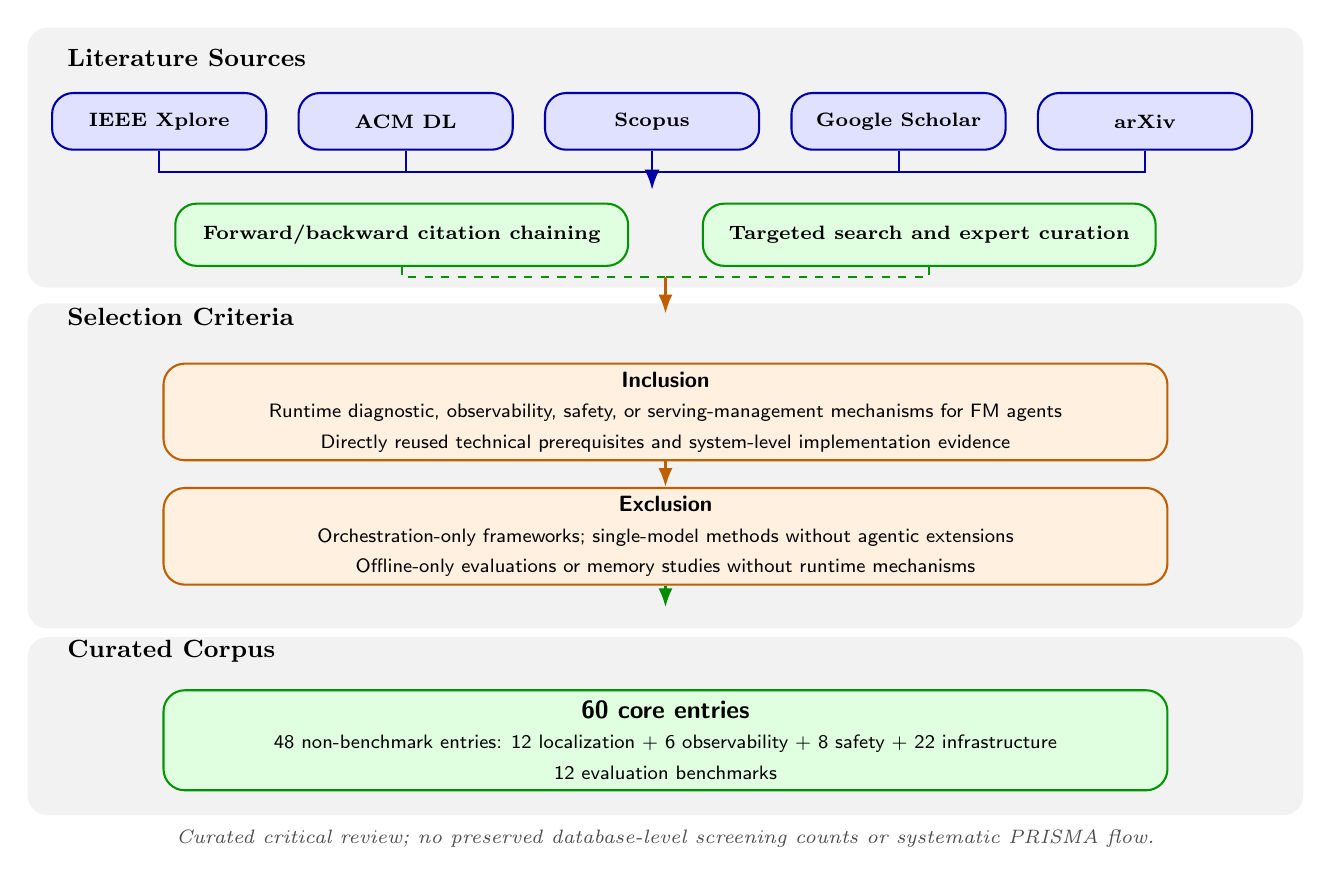
\begin{tikzpicture}[x=1cm,y=1cm,font=\sffamily,
  >={Latex[length=2mm,width=1.3mm]},
  bluebox/.style={rounded corners=2.7mm,draw=blue!65!black,fill=blue!12,line width=.75pt,align=center,inner sep=2pt},
  greenbox/.style={rounded corners=2.7mm,draw=green!58!black,fill=green!12,line width=.75pt,align=center,inner sep=3pt},
  amberbox/.style={rounded corners=2.7mm,draw=orange!75!black,fill=orange!12,line width=.75pt,align=center,inner sep=3pt},
  flowblue/.style={draw=blue!65!black,line width=.95pt,-Latex},
  flowgreen/.style={draw=green!55!black,line width=.85pt,-Latex},
  flowamber/.style={draw=orange!75!black,line width=.85pt,-Latex}]
\fill[black!5,rounded corners=2.5mm] (0,6.85) rectangle (16.2,10.15);
\node[anchor=west,font=\bfseries\small] at (.38,9.77) {Literature Sources};
\node[bluebox,minimum width=2.72cm,minimum height=.72cm,font=\bfseries\scriptsize] (ieee) at (1.67,8.96) {IEEE Xplore};
\node[bluebox,minimum width=2.72cm,minimum height=.72cm,font=\bfseries\scriptsize] (acm) at (4.80,8.96) {ACM DL};
\node[bluebox,minimum width=2.72cm,minimum height=.72cm,font=\bfseries\scriptsize] (scopus) at (7.93,8.96) {Scopus};
\node[bluebox,minimum width=2.72cm,minimum height=.72cm,font=\bfseries\scriptsize] (scholar) at (11.06,8.96) {Google Scholar};
\node[bluebox,minimum width=2.72cm,minimum height=.72cm,font=\bfseries\scriptsize] (arxiv) at (14.19,8.96) {arXiv};
\foreach \boxname in {ieee,acm,scopus,scholar,arxiv} {\draw[blue!65!black,line width=.7pt] (\boxname.south) -- ++(0,-.28);}
\draw[blue!65!black,line width=.75pt] (1.67,8.32) -- (14.19,8.32);
\draw[flowblue] (7.93,8.32) -- (7.93,8.09);
\node[greenbox,minimum width=5.75cm,minimum height=.79cm,font=\bfseries\scriptsize] (chain) at (4.75,7.52) {Forward/backward citation chaining};
\node[greenbox,minimum width=5.75cm,minimum height=.79cm,font=\bfseries\scriptsize] (target) at (11.45,7.52) {Targeted search and expert curation};
\draw[green!58!black,dashed,line width=.8pt] (chain.south) -- (4.75,6.98) -- (8.1,6.98);
\draw[green!58!black,dashed,line width=.8pt] (target.south) -- (11.45,6.98) -- (8.1,6.98);

\fill[black!5,rounded corners=2.5mm] (0,2.52) rectangle (16.2,6.65);
\node[anchor=west,font=\bfseries\small] at (.38,6.48) {Selection Criteria};
\draw[flowamber] (8.1,6.98) -- (8.1,6.52);
\node[amberbox,minimum width=12.75cm,minimum height=1.20cm] (include) at (8.1,5.27) {
  {\bfseries\footnotesize Inclusion}\\[-1pt]
  {\scriptsize Runtime diagnostic, observability, safety, or serving-management mechanisms for FM agents}\\[-1pt]
  {\scriptsize Directly reused technical prerequisites and system-level implementation evidence}
};
\node[amberbox,minimum width=12.75cm,minimum height=1.20cm] (exclude) at (8.1,3.69) {
  {\bfseries\footnotesize Exclusion}\\[-1pt]
  {\scriptsize Orchestration-only frameworks; single-model methods without agentic extensions}\\[-1pt]
  {\scriptsize Offline-only evaluations or memory studies without runtime mechanisms}
};
\draw[flowamber] (include.south) -- (exclude.north);
\draw[flowgreen] (8.1,3.06) -- (8.1,2.79);

\fill[black!5,rounded corners=2.5mm] (0,.15) rectangle (16.2,2.41);
\node[anchor=west,font=\bfseries\small] at (.38,2.23) {Curated Corpus};
\node[greenbox,minimum width=12.75cm,minimum height=1.27cm,align=center] at (8.1,1.10) {
  {\bfseries\small 60 core entries}\\[-1pt]
  {\scriptsize 48 non-benchmark entries: 12 localization + 6 observability + 8 safety + 22 infrastructure}\\[-1pt]
  {\scriptsize 12 evaluation benchmarks}
};
\node[font=\itshape\scriptsize,text=black!70] at (8.1,-.15)
  {Curated critical review; no preserved database-level screening counts or systematic PRISMA flow.};
\end{tikzpicture}
}
\caption{Curated corpus assembly. Blue boxes denote literature sources; green boxes show
chaining/curation and the final corpus; ochre boxes summarize selection rules.
This is a curated critical review, not a PRISMA systematic review: no
unsupported database screening counts are shown.}
\label{fig:v5_corpus_flow}
\end{figure}
\endgroup



\begin{thebibliography}{999}
\bibitem{v5ref1} Reyna Abhyankar, Zijian He, Vikranth Srivatsa, Hao Zhang, and Yiying Zhang. InferCept: Efficient intercept support for augmented large language model inference. In Proceedings of the 41st International Conference on Machine Learning (ICML), volume 235 of PMLR, pages 81--95, 2024. arXiv:2402.01869.
\bibitem{v5ref2} Adam AlSayyad, Kelvin Yuxiang Huang, and Richik Pal. AgentTrace: A structured logging framework for agent system observability. In AAAI 2026 Workshop on LLM-based Multi-Agent Systems (LaMAS), 2026. arXiv:2602.10133.
\bibitem{v5ref3} Shraddha Barke, Arnav Goyal, Alind Khare, Avaljot Singh, Suman Nath, and Chetan Bansal. AgentRx: Diagnosing AI agent failures from execution trajectories. In Findings of the Association for Computational Linguistics: EMNLP 2026, 2026. arXiv:2602.02475.
\bibitem{v5ref4} Zhuohang Bian, Feiyang Wu, Zhuoran Li, Teng Ma, and Youwei Zhuo. TokenCake: A KV-cache-centric serving framework for LLM-based multi-agent applications. In Pro- ceedings of the 20th European Conference on Computer Systems (EuroSys), 2027. doi: 10.1145/3842654.3848547. arXiv:2510.18586.
\bibitem{v5ref5} Mert Cemri, Melissa Z. Pan, Shuyi Yang, Lakshya A. Agrawal, Bhavya Chopra, Rishabh Tiwari, Kurt Keutzer, Aditya Parameswaran, Dan Klein, Kannan Ramchandran, Matei Zaharia, Joseph E. Gonzalez, and Ion Stoica. Why do multi-agent LLM systems fail? In NeurIPS 2025 Datasets and Benchmarks Track, 2025. arXiv:2503.13657. Spotlight.
\bibitem{v5ref6} Mengzhuo Chen, Junjie Wang, Fangwen Mu, Yawen Wang, Zhe Liu, Huanxiang Feng, and Qing Wang. Seeing the whole elephant: A benchmark for failure attribution in LLMbased multi-agent systems. arXiv preprint arXiv:2604.22708, 2026.
\bibitem{v5ref7} Weize Chen et al. Internet of agents: Weaving a web of heterogeneous agents for collaborative intelligence. arXiv preprint arXiv:2407.07061, 2024.
\bibitem{v5ref8} Zhaorun Chen, Mintong Kang, and Bo Li. ShieldAgent: Shielding agents via verifiable safety policy reasoning. In Proceedings of the 42nd International Conference on Machine Learning (ICML), volume 267 of PMLR, pages 8313--8344, 2025. arXiv:2503.22738.
\bibitem{v5ref9} Sahana Chennabasappa, Cyrus Nikolaidis, Daniel Song, David Molnar, Stephanie Ding, Shengye Wan, Spencer Whitman, Lauren Deason, Nicholas Doucette, Abraham Montilla, et al. LlamaFirewall: An open source guardrail system for building secure AI agents. arXiv preprint arXiv:2505.03574, 2025.
\bibitem{v5ref10} Darshan Deshpande, Varun Gangal, Hersh Mehta, Jitin Krishnan, Anand Kannappan, and Rebecca Qian. TRAIL: Trace reasoning and agentic issue localization. arXiv preprint arXiv:2505.08638, 2025.
\bibitem{v5ref11} Yu Ge, Linna Xie, Zhong Li, Yu Pei, and Tian Zhang. Who is introducing the failure? automatically attributing failures of multi-agent systems via spectrum analysis. arXiv preprint arXiv:2509.13782, 2025.
\bibitem{v5ref12} Xu He, Di Wu, Yan Zhai, and Kun Sun. SentinelAgent: Graph-based anomaly detection in multi-agent systems. arXiv preprint arXiv:2505.24201, 2025.
\bibitem{v5ref13} Sirui Hong, Mingchen Zhuge, Jonathan Chen, Xiawu Zheng, Yuheng Cheng, Ceyao Zhang, Jinlin Wang, Zili Wang, Steven Ka Shing Yau, Zijuan Lin, et al. MetaGPT: Meta programming for a multi-agent collaborative framework. arXiv preprint arXiv:2308.00352, 2023.
\bibitem{v5ref14} Woosuk Kwon, Zhuohan Li, Siyuan Zhuang, Ying Sheng, Lianmin Zheng, Cody Hao Yu, Joseph E. Gonzalez, Hao Zhang, and Ion Stoica. Efficient memory management for large language model serving with PagedAttention. In SOSP, 2023.
\bibitem{v5ref15} Guohao Li, Hasan Abed Al Kader Hammoud, Hani Itani, Dmitrii Khizbullin, and Bernard Ghanem. CAMEL: Communicative agents for ``mind'' exploration of large language model society. arXiv preprint arXiv:2303.17760, 2023.
\bibitem{v5ref16} Hanchen Li, Qiuyang Mang, Runyuan He, Qizheng Zhang, Huanzhi Mao, Xiaokun Chen, Hangrui Zhou, Alvin Cheung, Joseph E. Gonzalez, and Ion Stoica. Continuum: Efficient and robust multi-turn LLM agent scheduling with KV cache time-to-live. In ICLR 2026 Workshop: Lifelong Agents, 2026. arXiv:2511.02230. Also UC Berkeley Tech Report EECS-2026-234.
\bibitem{v5ref17} Chaofan Lin, Zhenhua Han, Chengruidong Zhang, Yuqing Yang, Fan Yang, Chen Chen, and Lili Qiu. Parrot: Efficient serving of LLM-based applications with semantic variable. In Proceedings of the 18th USENIX Symposium on Operating Systems Design and Implementation (OSDI), 2024. arXiv:2405.19888.
\bibitem{v5ref18} Dongrui Liu, Yu Li, Zhonghao Yang, Peng Wang, Guanxu Chen, et al. AgentDoG 1.5: A lightweight and scalable alignment framework for AI agent safety. arXiv preprint arXiv:2605.29801, 2026.
\bibitem{v5ref19} Yang Liu, Hongjiang Feng, Junsong Pu, and Zhuangbin Chen. MASPrism: Lightweight failure attribution for multi-agent systems using prefill-stage signals. arXiv preprint arXiv:2605.07509, 2026.
\bibitem{v5ref20} Yuhan Liu, Yuyang Huang, Jiayi Yao, Shaoting Feng, Zhuohan Gu, Kuntai Du, Hanchen Li, Yihua Cheng, Junchen Jiang, Shan Lu, Madan Musuvathi, and Esha Choukse. Droid- Speak: KV cache sharing for cross-LLM communication and multi-LLM serving. arXiv preprint arXiv:2411.02820, 2024.
\bibitem{v5ref21} Weidi Luo, Shenghong Dai, Xiaogeng Liu, Suman Banerjee, Huan Sun, Muhao Chen, and Chaowei Xiao. AGrail: A lifelong agent guardrail with effective and adaptive safety detection. arXiv preprint arXiv:2502.11448, 2025.
\bibitem{v5ref22} Ming Ma, Jue Zhang, Fangkai Yang, Yu Kang, Qingwei Lin, Saravan Rajmohan, and Dongmei Zhang. DoVer: Intervention-driven auto debugging for LLM multi-agent systems. arXiv preprint arXiv:2512.06749, 2025.
\bibitem{v5ref23} Akshay Manglik, Vijay S. Kalmath, Jason Qin, Apaar Shanker, Kaustubh Deshpande, Yash Maurya, Veronica Chatrath, Levi Lentz, and Yuan Xue. Insights generator: Systematic corpus-level trace diagnostics for LLM agents. arXiv preprint arXiv:2605.21347, 2025.
\bibitem{v5ref24} Hongqiu Ni, Han Tian, Chi Zhang, Guopeng Li, and Haisheng Tan. TOPAS: Workflow-aware prefix-state scheduling for multi-agent LLM serving. arXiv preprint arXiv:2608.25523, 2026.
\bibitem{v5ref25} OpenTelemetry GenAI SIG. OpenTelemetry semantic conventions for generative AI. https://github.com/open-telemetry/ semantic-conventions-genai, 2024. Specification.
\bibitem{v5ref26} Matthew J. Page, Joanne E. McKenzie, Patrick M. Bossuyt, Isabelle Boutron, Tammy C. Hoffmann, Cynthia D. Mulrow, Larissa Shamseer, Jennifer M. Tetzlaff, Elie A. Akl, Sue E. Brennan, et al. The PRISMA 2020 statement: an updated guideline for reporting systematic reviews. BMJ, 372:n71, 2021. doi: 10.1136/bmj.n71.
\bibitem{v5ref27} Zaifeng Pan, Ajjkumar Patel, Zhengding Hu, Yipeng Shen, Yue Guan, Wan-Lu Li, Lianhui Qin, Yida Wang, and Yufei Ding. KVFlow: Efficient prefix caching for accelerating LLM-based multi-agent workflows. In Proceedings of the 39th Conference on Neural Information Processing Systems (NeurIPS), 2025. arXiv:2507.07400.
\bibitem{v5ref28} Zaifeng Pan, Yipeng Shen, Zhengding Hu, Zhuang Wang, Aninda Manocha, Zheng Wang, Zhongkai Yu, Yue Guan, and Yufei Ding. ScaleSim: Serving large-scale multiagent simulation with invocation distance-based memory management. arXiv preprint arXiv:2601.21473, 2026.
\bibitem{v5ref29} Ravi Pandya, Madison Bland, Duy P. Nguyen, Changliu Liu, Jaime Fernández Fisac, and Andrea Bajcsy. ReGuard: From refusal to recovery: A control-theoretic approach to generative AI guardrails. arXiv preprint arXiv:2510.13727, 2025.
\bibitem{v5ref30} Chen Qian, Xin Cong, Cheng Yang, Weize Chen, Yusheng Su, Juyuan Xu, Zhiyuan Liu, and Maosong Sun. ChatDev: Communicative agents for software development. arXiv preprint arXiv:2307.07924, 2023.
\bibitem{v5ref31} Hezhe Qiao, Hanghang Tong, Ee-Peng Lim, Bing Liu, and Guansong Pang. VerifyMAS: Hypothesis verification for failure attribution in LLM-based multi-agent systems. In Proceedings of the 40th Conference on Neural Information Processing Systems (NeurIPS), 2026. arXiv:2605.17467.
\bibitem{v5ref32} Ruoyu Qin, Zheming Li, Weiran He, Jialei Cui, Feng Ren, Mingxing Zhang, Yongwei Wu, Weimin Zheng, and Xinran Xu. Mooncake: Trading more storage for less computation --- a KVCache-centric architecture for serving LLM chatbot. In Proceedings of the 23rd USENIX Conference on File and Storage Technologies (FAST), pages 155--170, 2025. arXiv:2407.00079. Erik Riedel Best Paper Award.
\bibitem{v5ref33} Md Nakhla Rafi, Md Ahasanuzzaman, Dong Jae Kim, Zhijie Wang, and Tse-Hsun Chen. FALAT: Tracing failures in LLM agent trajectories via dependency-guided search. arXiv preprint arXiv:2606.00765, 2026.
\bibitem{v5ref34} Ruxue Shi, Yili Wang, Mengnan Du, Qinggang Zhang, Rui Miao, Yixin Liu, and Xin Wang. SAIGuard: Communication-state simulation for proactive defense of LLM multiagent systems. arXiv preprint arXiv:2606.12474, 2026.
\bibitem{v5ref35} Minxing Wang, Xiaofei Xie, and Yintong Huo. TrajAudit: Automated failure diagnosis for agentic coding systems. arXiv preprint arXiv:2605.26563, 2026.
\bibitem{v5ref36} Shao Wang, Rui Ren, and Lin Gui. ForkKV: Scaling multi-LoRA agent serving via copyon-write disaggregated KV cache. arXiv preprint arXiv:2604.06370, 2026.
\bibitem{v5ref37} Shilong Wang, Guibin Zhang, Miao Yu, Guancheng Wan, Fanci Meng, Chongye Guo, Kun Wang, and Yang Wang. G-Safeguard: A topology-guided security lens and treatment on LLM-based multi-agent systems. In Proceedings of the 63rd Annual Meeting of the Association for Computational Linguistics (ACL), pages 7261--7276, 2025. arXiv:2502.11127.
\bibitem{v5ref38} Yawen Wang, Wenjie Wu, Junjie Wang, and Qing Wang. From flat logs to causal graphs: Hierarchical failure attribution for LLM-based multi-agent systems. arXiv preprint arXiv:2602.23701, 2026.
\bibitem{v5ref39} Yiqi Wang, Jiaqi Zhang, Zhangkai Wu, Taotao Cai, Zirui Liu, Zequn Sun, Mingkai Zheng, Manqing Dong, Yu-Xuan Qiu, Xuefei Yin, and Yanming Zhu. From agent traces to trust: A survey of evidence tracing and execution provenance in LLM agents. arXiv preprint arXiv:2606.04990, 2026.
\bibitem{v5ref40} Yufei Xia, Anjun Gao, Yueyang Quan, Zhuqing Liu, and Minghong Fang. Who broke the system? failure localization in LLM-based multi-agent systems. In Proceedings of the Conference on Language Modeling (COLM), 2026. arXiv:2607.07989.
\bibitem{v5ref41} Jiayi Yao, Hanchen Li, Yuhan Liu, Siddhant Ray, Yihua Cheng, Qizheng Zhang, Kuntai Du, Shan Lu, and Junchen Jiang. CacheBlend: Fast large language model serving for RAG with cached knowledge fusion. In Proceedings of the 20th European Conference on Computer Systems (EuroSys), 2025. arXiv:2405.16444.
\bibitem{v5ref42} Shunyu Yao, Noah Shinn, Pedram Razavi, and Karthik Narasimhan. $\tau$-bench: A benchmark for tool-agent-user interaction in real-world domains. arXiv preprint arXiv:2406.12045, 2024.
\bibitem{v5ref43} Hancheng Ye, Zhengqi Gao, Mingyuan Ma, Qinsi Wang, Yuzhe Fu, Ming-Yu Chung, Yueqian Lin, Zhijian Liu, Jianyi Zhang, Danyang Zhuo, and Yiran Chen. KVCOMM: Online cross-context KV-cache communication for efficient LLM-based multi-agent systems. In Proceedings of the 39th Conference on Neural Information Processing Systems (NeurIPS), 2025. arXiv:2510.12872.
\bibitem{v5ref44} Yichao Yuan, Mosharaf Chowdhury, and Nishil Talati. KAIROS: Stateful, context-aware power-efficient agentic inference serving. arXiv preprint arXiv:2604.16682, 2026.
\bibitem{v5ref45} Guibin Zhang, Junhao Wang, Junjie Chen, Wangchunshu Zhou, Kun Wang, and Shuicheng Yan. AgenTracer: Who is inducing failure in the LLM agentic systems? arXiv preprint arXiv:2509.03312, 2025. ICLR 2026.
\bibitem{v5ref46} Lvmin Zhang and Maneesh Agrawala. View-oriented conversation compiler for agent trace analysis. arXiv preprint arXiv:2603.29678, 2026.
\bibitem{v5ref47} Rui Zhang, Chaeeun Kim, and Liting Hu. A policy-driven runtime layer for agentic LLM serving. arXiv preprint arXiv:2605.27744, 2026.
\bibitem{v5ref48} Shaokun Zhang, Ming Yin, Jieyu Zhang, Jiale Liu, Zhiguang Han, Jingyang Zhang, Beibin Li, Chi Wang, Huazheng Wang, Yiran Chen, and Qingyun Wu. Which agent causes task failures and when? on automated failure attribution of LLM multi-agent systems. arXiv preprint arXiv:2505.00212, 2025.
\bibitem{v5ref49} Lianmin Zheng, Liangsheng Yin, Zhiqiang Xie, Chuyue Sun, Jeff Huang, Cody Hao Yu, Shiyi Cao, Christos Kozyrakis, Ion Stoica, Joseph E. Gonzalez, Clark Barrett, and Ying Sheng. SGLang: Efficient execution of structured language model programs. In Advances in Neural Information Processing Systems, volume 37 (NeurIPS 2024). arXiv:2312.07104.
\bibitem{v5ref50} Yinmin Zhong, Shengyu Liu, Junda Chen, Jianbo Hu, Yibo Zhu, Xuanzhe Liu, Xin Jin, and Hao Zhang. DistServe: Disaggregating prefill and decoding for goodput-optimized large language model serving. In Proceedings of the 18th USENIX Symposium on Operating Systems Design and Implementation (OSDI), 2024. arXiv:2401.09670.
\bibitem{v5ref51} Chenyang Zhu, Spencer Hong, Jingyu Wu, Kushal Chawla, Charlotte Tang, Youbing Yin, Nathan Wolfe, Erin Babinsky, and Daben Liu. RAFFLES: Reasoning-based attribution of faults for LLM systems. arXiv preprint arXiv:2509.06822, 2025.
\bibitem{v5ref52} Taiyu Zhu, Yifan Wu, Weilin Jin, Ying Li, and Gang Huang. StepFinder: A temporal semantic framework for failure attribution in multi-agent systems. In Proceedings of the 32nd ACM SIGKDD Conference on Knowledge Discovery and Data Mining (KDD), 2026. arXiv:2606.03467.
\bibitem{v5supp1} LangChain. LangSmith Observability Documentation. https://docs.smith.langchain.com/observability.
\bibitem{v5supp2} Zhuohang Bian et al. TokenDance: Scaling Multi-Agent LLM Serving via Collective KV Cache Sharing. arXiv:2604.03143, 2026.
\bibitem{v5supp3} Bole Ma, Jan Eitzinger, Harald Koestler. Leyline: KV Cache Directives for Agentic Inference. arXiv:2606.01065, 2026.
\bibitem{v5supp4} Hyesung Jeon et al. LRAgent: Efficient KV Cache Sharing for Multi-LoRA LLM Agents. ICML 2026, PMLR 306.
\bibitem{v5supp5} Ishan Patel and Ishan Joshi. PolyKV: A Shared Asymmetrically-Compressed KV Cache Pool for Multi-Agent LLM Inference. arXiv:2604.24971, 2026.
\bibitem{v5supp6} Yifan Qiao et al. ConServe: Fine-Grained GPU Harvesting for LLM Online and Offline Co-Serving. ICML 2026, PMLR 306.
\bibitem{v5supp7} Kunlun Zhu et al. MultiAgentBench: Evaluating the Collaboration and Competition of LLM Agents. ACL 2025.
\bibitem{v5supp8} Vishal Ishwar Naik et al. GuardianAgentBench: Where Agents Fail and How to Guard Them. arXiv:2607.20982, 2026.
\bibitem{v5supp9} Aayush Gupta. ReliabilityBench: Evaluating LLM Agent Reliability Under Production-Like Stress Conditions. arXiv:2601.06112, 2026.
\bibitem{v5supp10} Zhexin Zhang et al. Agent-SafetyBench: Evaluating Safety of LLM Agents. arXiv:2412.14470, 2024.
\bibitem{v5supp11} Maksym Andriushchenko et al. AgentHarm: A Benchmark for Measuring Harmfulness of LLM Agents. ICLR 2025.
\bibitem{v5supp12} Ishan Kavathekar et al. TAMAS: Benchmarking Adversarial Risks in Multi-Agent LLM Systems. ACL 2026.
\bibitem{v5supp13} Hanrong Zhang et al. Agent Security Bench (ASB): Formalizing and Benchmarking Attacks and Defenses in LLM-based Agents. ICLR 2025.
\bibitem{v5supp14} Mina Mohammadmirzaei and Jeffrey Flanigan. OSGuard: A Benchmark for Safety in Computer-Use Agents. arXiv:2606.15034, 2026.
\bibitem{survey_lifecycle} Chen Kang and Kunyan Li. A lifecycle-oriented survey of LLM-based agents: Workflow, graph augmentation, and future directions. Neurocomputing 704, 134838, 2026. \url{https://doi.org/10.1016/j.neucom.2026.134838}.
\bibitem{survey_agentic} Smita Khapre, Melkamu Abay Mersha, Zainab Olalekan, Hassan Shakil, Samer Iskander, Asser Moustafa, and Jugal Kalita. Agentic AI systems: A systematic survey of multi-agent architectures, cognitive foundations, interaction, explainability, security, and performance evaluation. Neurocomputing 696, 134049, 2026. \url{https://doi.org/10.1016/j.neucom.2026.134049}.
\bibitem{survey_graph} Panpan Zhou, Haowei Zhu, Liwei Li, Yan Liang, Kaibing Yin, Lixiang Xu, Mingru Lei, and Yuhua Chen. Large language models meet graph neural networks: A survey. Neurocomputing 710, 135372, 2027. \url{https://doi.org/10.1016/j.neucom.2026.135372}.
\bibitem{survey_embodied} Rui Zhou, Wenlong Liang, Yang Ma, Bing Zhang, Songlin Li, Yijia Liao, and Ping Kuang. Large model empowered embodied AI: A survey on decision-making and embodied learning. Neurocomputing 711, 135458, 2027. \url{https://doi.org/10.1016/j.neucom.2026.135458}.
\bibitem{survey_serving} Hanbo Ma, Zhongguo Li, Junan Wang, Chunyi Cao, Donglin Li, Jun Yang, and Zhengtao Ding. Load balancing for large language model inference serving: A control and learning oriented survey. Neurocomputing 706, 134973, 2026. \url{https://doi.org/10.1016/j.neucom.2026.134973}.
\bibitem{survey_edge_rag} Zhiyuan Cheng, Longying Lai, Yue Liu, and Yu Sun. Toward sustainable on-device intelligence: A survey on energy-efficient RAG systems with small language models. Research Square preprint, 2026. \url{https://doi.org/10.21203/rs.3.rs-10597421/v1}.
\bibitem{survey_humor} Tuo Liang, Zhe Hu, Disheng Liu, Juncheng Wang, Jing Li, and Yu Yin. Computational humor with multimodal LLMs: Methods, datasets, evaluation, and challenges. arXiv preprint, 2026. \url{https://arxiv.org/abs/2607.19011}.
% Restored and expanded contextual references, 2026-11-17
% These records supplement the original V5 reference entries.
% Source: original manuscript's retained BibTeX + two public bibliographic datasets.
% Locator metadata is available, but full-text paper-by-paper claims are NOT certified.
% References are cited in the supplementary coverage map below; none is
% silently promoted to Tier 1 of the 60-entry core evidence census.

\bibitem{ext001} Dong Ho Kang, Hyeonjeong Cha, Daein Weon. Knowledge-Based Zero-Replay Debugging for Multi-Agent Systems. arXiv preprint arXiv:2606.14805, 2026. \url{https://arxiv.org/abs/2606.14805}.

\bibitem{ext002} Xuyan Ma, Yawen Wang et al. Diagnosis-Driven Automatic Repair for Multi-Agent Systems. arXiv preprint arXiv:2607.02882, 2026. \url{https://arxiv.org/abs/2607.02882}.

\bibitem{ext003} Jiale Liu, Huajun Xi et al. {Who\&When Pro}: Meta-evaluation of Failure Attribution in Multi-Agent Systems. arXiv preprint arXiv:2607.09996, 2026. \url{https://arxiv.org/abs/2607.09996}.

\bibitem{ext004} Adi Banerjee, Anirudh Nair, Tarik Borogovac. Where Did It All Go Wrong? Hierarchical Error Attribution in Multi-Agent Systems. arXiv preprint arXiv:2510.04886, 2025. \url{https://arxiv.org/abs/2510.04886}.

\bibitem{ext005} Will Epperson, Gagan Bansal et al. Interactive Debugging and Steering for Multi-Agent Systems. CHI, 2025. \url{https://arxiv.org/abs/2503.02068}.

\bibitem{ext006} Netta Madvil, Gilad Dym et al. Holistic Evaluation and Failure Diagnosis for {LLM} Agents. arXiv preprint arXiv:2605.14865, 2026. \url{https://arxiv.org/abs/2605.14865}.

\bibitem{ext007} Chenyu Zhao, Shenglin Zhang et al. {AgentTether}: Graph-Guided Diagnosis and Intervention for Agents. arXiv preprint arXiv:2607.06273, 2026. \url{https://arxiv.org/abs/2607.06273}.

\bibitem{ext008} Shihao Qi, Jie Ma et al. Beyond Individual Intelligence: A Survey on Collaboration and Failure in Multi-Agent Systems. arXiv preprint arXiv:2605.14892, 2026. \url{https://arxiv.org/abs/2605.14892}.

\bibitem{ext009} Twinkll Sisodia. {AI} Observability: A Multi-Layer Survey. arXiv preprint arXiv:2604.26152, 2026. \url{https://arxiv.org/abs/2604.26152}.

\bibitem{ext011} Liming Dong, Qinghua Lu, Liming Zhu. {AgentOps}: Enabling Observability of {LLM} Agents. arXiv preprint arXiv:2411.05285, 2024. \url{https://arxiv.org/abs/2411.05285}.

\bibitem{ext012} Zexin Wang, Changhua Pei et al. Agent System Operations: Lifecycle Management for {LLM} Agents. arXiv preprint arXiv:2606.01581, 2026. \url{https://arxiv.org/abs/2606.01581}.

\bibitem{ext013} Shaunak Biswas, Hiya Bhatt, Karthik Vaidhyanathan. Architecting {AgentOps}: Design Patterns for {LLM} Agent Operations. arXiv preprint arXiv:2601.06456, 2026. \url{https://arxiv.org/abs/2601.06456}.

\bibitem{ext014} Fabiana Fournier, Lior Limonad, Yuval David. Agentic {AI} Process Observability via Process Mining. arXiv preprint arXiv:2505.20127, 2025. \url{https://arxiv.org/abs/2505.20127}.

\bibitem{ext015} Yi Nian, Aojie Yuan et al. Auditable Agents: Unified Graph for Security Auditing. arXiv preprint arXiv:2604.05485, 2026. \url{https://arxiv.org/abs/2604.05485}.

\bibitem{ext016} Chaofan Li, Lyuye Zhang, Jintao Zhai et al. Towards Security-Auditable {LLM} Agents: A Unified Graph Representation. arXiv preprint arXiv:2605.06812, 2026. \url{https://arxiv.org/abs/2605.06812}.

\bibitem{ext017} Pierre Dantas, Lucas Cordeiro, Ehsan Nowroozi et al. Toward Safe {LLM} Agents: A Survey of Specification, Verification, and Enforcement. arXiv preprint arXiv:2608.14590, 2026. \url{https://arxiv.org/abs/2608.14590}.

\bibitem{ext018} Miao Yu, Fanci Meng, Xinyun Zhou et al. A Survey on Trustworthy {LLM} Agents: Threats and Countermeasures. KDD, 2025. \url{https://arxiv.org/abs/2503.09648}.

\bibitem{ext019} Zhen Xiang, Linzhi Zheng, Yanjie Li et al. {GuardAgent}: Safeguard {LLM} Agents by a Guard Agent via Knowledge-Enabled Reasoning. arXiv preprint arXiv:2406.09187, 2024. \url{https://arxiv.org/abs/2406.09187}.

\bibitem{ext020} Lesly Miculicich, Mihir Parmar, Hamid Palangi et al. {VeriGuard}: Enhancing {LLM} Agent Safety via Verified Code Generation. arXiv preprint arXiv:2510.05156, 2025. \url{https://arxiv.org/abs/2510.05156}.

\bibitem{ext021} Hanjun Luo, Shenyu Dai, Chiming Ni et al. {AgentAuditor}: Automated Auditing of {LLM} Agent Safety. NeurIPS, 2025. \url{https://arxiv.org/abs/2506.00641}.

\bibitem{ext022} Kun Wang, Guibin Zhang, Zhenhong Zhou et al. A Comprehensive Survey in {LLM}(-Agent) Full Stack Safety: Data, Training and Deployment. arXiv preprint arXiv:2504.15585, 2025. \url{https://arxiv.org/abs/2504.15585}.

\bibitem{ext025} Haoyu Zheng, Fangcheng Fu, Jia Wu et al. Efficient Serving for Dynamic Agent Workflows with Prediction-based {KV}-Cache Management. arXiv preprint arXiv:2605.06472, 2026. \url{https://arxiv.org/abs/2605.06472}.

\bibitem{ext026} Jie Li, Tongyang Wang, Yong Chen. From Tensor Buffer to Distributed Memory Hierarchy: A Survey of {KV} Cache Management for {LLM} Serving. arXiv preprint arXiv:2607.02574, 2026. \url{https://arxiv.org/abs/2607.02574}.

\bibitem{ext027} Yakov Pyotr Shkolnikov. Agent Memory Below the Prompt: Persistent {Q4} {KV} Cache for Multi-Agent {LLM} Inference on Edge Devices. arXiv preprint arXiv:2603.04428, 2026. \url{https://arxiv.org/abs/2603.04428}.

\bibitem{ext028} Michael Luo, Xiaoxiang Shi, Colin Cai et al. {Autellix}: An Efficient Serving Engine for {LLM} Agents. arXiv preprint arXiv:2502.13965, 2025. \url{https://arxiv.org/abs/2502.13965}.

\bibitem{ext029} Pengyu Zhu, Lijun Li, Yaxing Lyu et al. A Unified Framework for the Evaluation of {LLM} Agentic Capabilities. arXiv preprint arXiv:2605.27898, 2026. \url{https://arxiv.org/abs/2605.27898}.

\bibitem{ext030} Abdelghny Orogat, Ana Rostam, Essam Mansour. Understanding Multi-Agent {LLM} Frameworks: A Unified Benchmark and Experimental Analysis. arXiv preprint arXiv:2602.03128, 2026. \url{https://arxiv.org/abs/2602.03128}.

\bibitem{ext031} Shiwen Ni, Guhong Chen, Shuaimin Li et al. A Survey on Large Language Model Benchmarks. arXiv preprint arXiv:2508.15361, 2025. \url{https://arxiv.org/abs/2508.15361}.

\bibitem{ext032} Haishan Lin, Hoilam Pao, Shaoxiong Zhan et al. Model-Native Computing Architecture: Envisioning Future System Architecture Through the Lens of Computer Architecture. arXiv preprint arXiv:2606.00288, 2026. \url{https://arxiv.org/abs/2606.00288}.

\bibitem{ext033} Md Shamsujjoha, Qinghua Lu, Dehai Zhao et al. Swiss Cheese Model for {AI} Safety: A Taxonomy and Reference Architecture for Multi-Layered Guardrails of Foundation Model Based Agents. IEEE ICSA, 2025. \url{https://doi.org/10.1109/ICSA65012.2025.00014}.

\bibitem{ext034} Zexin Wang, Jingjing Li, Quan Zhou et al. A Survey on {AgentOps}: Categorization, Challenges, and Future Directions. arXiv preprint arXiv:2508.02121, 2025. \url{https://arxiv.org/abs/2508.02121}.

\bibitem{ext035} Mohamad Abou Ali, Fadi Dornaika. Agentic {AI}: A Comprehensive Survey of Architectures, Applications, and Future Directions. Artificial Intelligence Review, 2025. \url{https://doi.org/10.1007/s10462-025-11422-4}.

\bibitem{ext036} Xinming Tu, Tianze Wang, Yingzhou Lu et al. {BenchGuard}: Who Guards the Benchmarks? Automated Auditing of {LLM} Agent Benchmarks. arXiv preprint arXiv:2604.24955, 2026. \url{https://arxiv.org/abs/2604.24955}.

\bibitem{ext037} Lingzhe Zhang, Tong Jia, Mingyu Wang et al. Efficient Failure Management for Multi-Agent Systems with Reasoning Trace Representation ({EAGER}). arXiv preprint arXiv:2603.21522, 2026. \url{https://arxiv.org/abs/2603.21522}.

\bibitem{ext038} Asaf Yehudai, Lilach Eden, Alan Li et al. A Survey on Evaluation of {LLM}-based Agents. Findings of the Association for Computational Linguistics: ACL 2026, 2026. \url{https://doi.org/10.18653/v1/2026.findings-acl.1330}.

\bibitem{ext039} Mahmoud Mohammadi, Yipeng Li, Jane Lo et al. Evaluation and Benchmarking of {LLM} Agents: A Survey. Proceedings of the 31st ACM SIGKDD Conference, 2025. \url{https://doi.org/10.1145/3711896.3736570}.

\bibitem{ext040} Ying Sheng, Lianmin Zheng, Binhang Yuan et al. {FlexGen}: High-Throughput Generative Inference of Large Language Models with a Single {GPU}. arXiv preprint arXiv:2303.06865, 2023. \url{https://arxiv.org/abs/2303.06865}.

\bibitem{ext041} Ahasan Kabir, Jiaqi Xue, Mengxin Zheng et al. {INFRAMIND}: Infrastructure-Aware Multi-Agent Orchestration. arXiv preprint arXiv:2606.11440, 2026. \url{https://arxiv.org/abs/2606.11440}.

\bibitem{ext042} Gyeongmuk Park, Seonghyeon Lee, Yeonsu Park. Minimizing Response Latency in {LLM}-Based Agent Systems: A Comprehensive Survey. IEEE Access, 2026. \url{https://doi.org/10.1109/ACCESS.2026.3664226}.

\bibitem{ext043} Xinyi Li, Sai Wang, Siqi Zeng et al. A Survey on {LLM}-based Multi-agent Systems: Workflow, Infrastructure, and Challenges. Vicinagearth, 2024. \url{https://doi.org/10.1007/s44336-024-00009-2}.

\bibitem{ext044} Saddek Bensalem, Yi Dong, Martin Fränzle et al. Position: A Three-Layer Probabilistic Assume-Guarantee Architecture Is Structurally Required for Safe {LLM} Agent Deployment. arXiv preprint arXiv:2605.18672, 2026. \url{https://arxiv.org/abs/2605.18672}.

\bibitem{ext045} Khanh-Tung Tran, Dung Dao, Minh-Duong Nguyen et al. Multi-Agent Collaboration Mechanisms: A Survey of {LLM}s. arXiv preprint arXiv:2501.06322, 2025. \url{https://arxiv.org/abs/2501.06322}.

\bibitem{ext046} Zixiang Wang, Mengjia Gong, Qiyu Sun et al. Multi-Agent Systems: From Classical Paradigms to Large Foundation Model-Enabled Futures. arXiv preprint arXiv:2604.18133, 2026. \url{https://arxiv.org/abs/2604.18133}.

\bibitem{ext048} Yiwen Zhu, Lihe Liu, Jiaqian Yu et al. {LLM}-Based Multi-Agent Orchestration: A Survey of Frameworks, Communication Protocols, and Emerging Patterns. Future Internet, 2026. \url{https://doi.org/10.3390/fi18060326}.

\bibitem{ext049} Vikranth Srivatsa, Zijian He, Reyna Abhyankar et al. Preble: Efficient Distributed Prompt Scheduling for {LLM} Serving. ICLR, 2025. \url{https://arxiv.org/abs/2407.00023}.

\bibitem{ext050} Amey Agrawal, Nitin Kedia, Ashish Panwar et al. Taming Throughput-Latency Tradeoff in {LLM} Inference with {Sarathi-Serve}. OSDI, 2024. \url{https://arxiv.org/abs/2403.02310}.

\bibitem{ext051} Ying Sheng, Shiyi Cao, Dacheng Li et al. {S-LoRA}: Serving Thousands of Concurrent {LoRA} Adapters. MLSys, 2024. \url{https://arxiv.org/abs/2311.03285}.

\bibitem{ext052} Bingyang Wu, Ruidong Zhu, Zili Zhang et al. {dLoRA}: Dynamically Orchestrating Requests and Adapters for {LoRA} {LLM} Serving. OSDI, 2024. \url{https://www.usenix.org/conference/osdi24/presentation/wu-bingyang}.

\bibitem{ext053} Boxuan Zhang, Jianing Zhu, Zeru Shi et al. {AgentForesight}: Online Auditing for Early Failure Prediction in Multi-Agent Systems. arXiv preprint arXiv:2605.08715, 2026. \url{https://arxiv.org/abs/2605.08715}.

\bibitem{ext054} Rui Miao, Yixin Liu, Yili Wang et al. {BlindGuard}: Safeguarding {LLM}-based Multi-Agent Systems under Unknown Attacks. arXiv preprint arXiv:2508.08127, 2025. \url{https://arxiv.org/abs/2508.08127}.

\bibitem{ext055} Yuanhao Li, Hongbo Wang, Xuhong Chen et al. {Counterfactual Rollout Replay: Forkable Environments as Free Process Rewards for Software Engineering Agents}. Preprint or technical documentation, 2026. \url{https://arxiv.org/abs/2609.33875}.

\bibitem{ext056} Yuanhao Li, Mingshan Liu, Hongbo Wang et al. {DRAFT-RL: Multi-Agent Chain-of-Draft Reasoning for Reinforcement Learning-Enhanced LLMs}. Proceedings of the AAAI Conference on Artificial Intelligence, 2026. \url{https://doi.org/10.1609/aaai.v40i35.40195}.

\bibitem{ext057} Yuanhao Li, Hongbo Wang, Xuhong Chen et al. {Retrieval-Augmented Multi-Agent Multimodal Framework for Fake News Detection}. ICASSP 2026, 2026. \url{https://cmsworkshops.com/ICASSP2026/view_paper.php?PaperNum=9709}.

\bibitem{ext058} Yuxuan Jiang, Runchao Li, Shubhashis Roy Dipta et al. Cornerstones or Stumbling Blocks? Deciphering the Rock Tokens in On-Policy Distillation. Preprint or technical documentation, 2026. \url{https://arxiv.org/abs/2605.09253}.

\bibitem{ext059} Jiang, Yuxuan, Li, Dawei, Ferraro, Francis. {DRP}: Distilled Reasoning Pruning with Mathematical Skill-aware Step Decomposition for Efficient Large Reasoning Models. Findings of the Association for Computational Linguistics: ACL 2026, 2026. \url{https://doi.org/10.18653/v1/2026.findings-acl.196}.

\bibitem{ext060} Jiang, Yuxuan, Ferraro, Francis. Beyond Math: Stories as a Testbed for Memorization-Constrained Reasoning in {LLM}s. Proceedings of the 19th Conference of the European Chapter of the Association for Computational Linguistics (Volume 1: Long Papers), 2026. \url{https://doi.org/10.18653/v1/2026.eacl-long.261}.

\bibitem{ext061} Yuxuan Jiang, Francis Ferraro. {SCRIBE}: Structured Mid-Level Supervision for Tool-Using Language Models. Preprint or technical documentation, 2026. \url{https://arxiv.org/abs/2601.03555}.

\bibitem{ext062} Yuxuan Jiang, Francis Ferraro. Bridging Reasoning Trajectories in On-Policy Distillation via Near-Future Guidance. Preprint or technical documentation, 2026. \url{https://arxiv.org/abs/2606.00305}.

\bibitem{ext063} Zhu, Junru, Xie, Shiming, Chen, Aime Lu Fan et al. Failure-Transparent Agents: Benchmarking Post-Failure Reporting in Tool-Using Language Models. arXiv preprint arXiv:2609.35732, 2026. \url{https://arxiv.org/abs/2609.35732}.

\bibitem{ext064} Zhu, Junru, Yang, Yixin, Ding, Xiaoqing et al. LeaseGuard: Incumbent-Preserving Admission Control for Privileged LLM Agents. arXiv preprint arXiv:2609.24077, 2026. \url{https://arxiv.org/abs/2609.24077}.

\bibitem{ext065} Wu, Qingyun, Bansal, Gagan, Zhang, Jieyu et al. AutoGen: Enabling Next-Gen LLM Applications via Multi-Agent Conversation. Preprint or technical documentation, 2023. \url{https://arxiv.org/abs/2308.08155}.

\bibitem{ext066} Chen, Weize, Su, Yusheng, Zuo, Jingwei et al. {AgentVerse}: Facilitating Multi-Agent Collaboration and Exploring Emergent Behaviors. Proceedings of the 12th International Conference on Learning Representations (ICLR), 2024. \url{https://arxiv.org/abs/2308.10848}.

\bibitem{ext067} Park, Joon Sung, O'Brien, Joseph C., Cai, Carrie J. et al. Generative Agents: Interactive Simulacra of Human Behavior. Proceedings of the 36th Annual ACM Symposium on User Interface Software and Technology (UIST), 2023. \url{https://arxiv.org/abs/2304.03442}.

\bibitem{ext068} Sumers, Theodore R., Yao, Shunyu, Narasimhan, Karthik et al. Cognitive Architectures for Language Agents. Preprint or technical documentation, 2023. \url{https://arxiv.org/abs/2309.02427}.

\bibitem{ext069} Du, Yilun, Li, Shuang, Torralba, Antonio et al. Improving Factuality and Reasoning in Language Models through Multiagent Debate. Proceedings of the 41st International Conference on Machine Learning (ICML), 2024. \url{https://arxiv.org/abs/2305.14325}.

\bibitem{ext070} Liang, Tian, He, Zhiwei, Jiao, Wenxiang et al. Encouraging Divergent Thinking in Large Language Models through Multi-Agent Debate. Proceedings of the 2024 Conference on Empirical Methods in Natural Language Processing (EMNLP), 2024. \url{https://arxiv.org/abs/2305.19118}.

\bibitem{ext071} Shinn, Noah, Cassano, Federico, Berman, Edward et al. Reflexion: Language Agents with Verbal Reinforcement Learning. Advances in Neural Information Processing Systems (NeurIPS), 2023. \url{https://arxiv.org/abs/2303.11366}.

\bibitem{ext072} Liu, Xiao, Yu, Hao, Zhang, Hanchen et al. {AgentBench}: Evaluating {LLM}s as Agents. Proceedings of the 12th International Conference on Learning Representations (ICLR), 2024. \url{https://arxiv.org/abs/2308.03688}.

\bibitem{ext073} Wang, Wei, Zhang, Dan, Feng, Tao et al. {BattleAgentBench}: A Benchmark for Evaluating Cooperation and Competition Capabilities of Language Models in Multi-Agent Systems. Preprint or technical documentation, 2024. \url{https://arxiv.org/abs/2408.15971}.

\bibitem{ext074} Qian, Chen, Xie, Zihao, Wang, YiFei et al. Scaling Large Language Model-based Multi-Agent Collaboration. Proceedings of the 13th International Conference on Learning Representations (ICLR), 2025. \url{https://arxiv.org/abs/2406.07155}.

\bibitem{ext075} He, Pengfei, Lin, Yupin, Dong, Shen et al. Red-Teaming {LLM} Multi-Agent Systems via Communication Attacks. Preprint or technical documentation, 2025. \url{https://arxiv.org/abs/2502.14847}.

\bibitem{ext076} Mou, Xinyi, Ding, Xuanwen, He, Qi et al. From Individual to Society: A Survey on Social Simulation Driven by Large Language Model-based Agents. Preprint or technical documentation, 2024. \url{https://arxiv.org/abs/2412.03563}.

\bibitem{ext077} Guo, Taicheng, Chen, Xiuying, Wang, Yaqi et al. Large Language Model based Multi-Agents: A Survey of Progress and Challenges. Proceedings of the 33rd International Joint Conference on Artificial Intelligence (IJCAI), 2024. \url{https://doi.org/10.24963/ijcai.2024/890}.

\bibitem{ext078} Han, Shanshan, Zhang, Qifan, Jin, Weizhao et al. {LLM} Multi-Agent Systems: Challenges and Open Problems. Preprint or technical documentation, 2024. \url{https://arxiv.org/abs/2402.03578}.

\bibitem{ext079} Lu, Jinliang, Pang, Ziliang, Xiao, Min et al. Merge, Ensemble, and Cooperate! A Survey on Collaborative Strategies in the Era of Large Language Models. Preprint or technical documentation, 2024. \url{https://arxiv.org/abs/2407.06089}.

\bibitem{ext080} Shen, Yongliang, Song, Kaitao, Tan, Xu et al. {HuggingGPT}: Solving {AI} Tasks with {ChatGPT} and its Friends in {Hugging Face}. Advances in Neural Information Processing Systems (NeurIPS), 2023. \url{https://arxiv.org/abs/2303.17580}.

\bibitem{ext081} Wang, Guanzhi, Xie, Yuqi, Jiang, Yunfan et al. Voyager: An Open-Ended Embodied Agent with Large Language Models. Preprint or technical documentation, 2023. \url{https://arxiv.org/abs/2305.16291}.

\bibitem{ext082} Abdelnabi, Sahar, Gomaa, Amr, Sivaprasad, Sarath et al. Cooperation, Competition, and Maliciousness: {LLM}-Stakeholders Interactive Negotiation. Preprint or technical documentation, 2023. \url{https://arxiv.org/abs/2309.17234}.

\bibitem{ext083} Bianchi, Federico, Chia, Patrick John, Yuksekgonul, Mert et al. How Well Can {LLM}s Negotiate? {NegotiationArena} Platform and Analysis. Proceedings of the 41st International Conference on Machine Learning (ICML), 2024. \url{https://arxiv.org/abs/2402.05863}.

\bibitem{ext084} Zhang, Hongxin, Du, Weihua, Shan, Jiaming et al. Building Cooperative Embodied Agents Modularly with Large Language Models. Proceedings of the 12th International Conference on Learning Representations (ICLR), 2024. \url{https://arxiv.org/abs/2307.02485}.

\bibitem{ext085} Wang, Junlin, Wang, Jue, Athiwaratkun, Ben et al. Mixture-of-Agents Enhances Large Language Model Capabilities. Preprint or technical documentation, 2024. \url{https://arxiv.org/abs/2406.04692}.

\bibitem{ext086} Yin, Zhangyue, Sun, Qiushi, Chang, Cheng et al. Exchange-of-Thought: Enhancing Large Language Model Capabilities through Cross-Model Communication. Proceedings of the 2023 Conference on Empirical Methods in Natural Language Processing (EMNLP), 2023. \url{https://aclanthology.org/2023.emnlp-main.936/}.

\bibitem{ext087} Liu, Zijun, Zhang, Yanzhe, Li, Peng et al. Dynamic {LLM}-Agent Network: An {LLM}-agent Collaboration Framework with Agent Team Optimization. Preprint or technical documentation, 2023. \url{https://arxiv.org/abs/2310.02170}.

\bibitem{ext088} {Altera.AL}, Ahn, Andrew, Becker, Nic et al. Project Sid: Many-agent Simulations Toward {AI} Civilization. Preprint or technical documentation, 2024. \url{https://arxiv.org/abs/2411.00114}.

\bibitem{ext089} Piao, Jinghua, Yan, Yuwei, Zhang, Jun et al. {AgentSociety}: Large-Scale Simulation of {LLM}-Driven Generative Agents Advances Understanding of Human Behaviors and Society. Preprint or technical documentation, 2025. \url{https://arxiv.org/abs/2502.08691}.

\bibitem{ext090} Zheng, Yi, Ma, Chongyang, Shi, Kanle et al. Agents Meet {OKR}: An Object and Key Results Driven Agent System with Hierarchical Self-Collaboration and Self-Evaluation. Preprint or technical documentation, 2023. \url{https://arxiv.org/abs/2311.16542}.

\bibitem{ext091} Li, Yuan, Zhang, Yixuan, Sun, Lichao. {MetaAgents}: Simulating Interactions of Human Behaviors for {LLM}-based Task-oriented Coordination via Collaborative Generative Agents. Preprint or technical documentation, 2023. \url{https://arxiv.org/abs/2310.06500}.

\bibitem{ext092} Yao, Shunyu, Yu, Dian, Zhao, Jeffrey et al. Tree of Thoughts: Deliberate Problem Solving with Large Language Models. Advances in Neural Information Processing Systems (NeurIPS), 2023. \url{https://arxiv.org/abs/2305.10601}.

\bibitem{ext093} Besta, Maciej, Blach, Nils, Kubicek, Ales et al. Graph of Thoughts: Solving Elaborate Problems with Large Language Models. Proceedings of the 38th AAAI Conference on Artificial Intelligence (AAAI), 2024. \url{https://arxiv.org/abs/2308.09687}.

\bibitem{ext094} Dong, Yihong, Jiang, Xue, Jin, Zhi et al. Self-collaboration Code Generation via {ChatGPT}. Preprint or technical documentation, 2023. \url{https://arxiv.org/abs/2304.07590}.

\bibitem{ext095} Wang, Zhenhailong, Mao, Shaoguang, Wu, Wenshan et al. Unleashing the Emergent Cognitive Synergy in Large Language Models: A Task-Solving Agent through Multi-Persona Self-Collaboration. Proceedings of the 2024 Annual Conference of the North American Chapter of the Association for Computational Linguistics (NAACL), 2024. \url{https://arxiv.org/abs/2307.05300}.

\bibitem{ext096} Liu, Junwei, Wang, Kaixin, Chen, Yixuan et al. Large Language Model-Based Agents for Software Engineering: A Survey. Preprint or technical documentation, 2024. \url{https://arxiv.org/abs/2409.02977}.

\bibitem{ext097} Li, Yang, Yu, Yangyang, Li, Haohang et al. {TradingGPT}: Multi-Agent System with Layered Memory and Distinct Characters for Enhanced Financial Trading Performance. Preprint or technical documentation, 2023. \url{https://arxiv.org/abs/2309.03736}.

\bibitem{ext098} Xiao, Yijia, Sun, Edward, Luo, Di et al. {TradingAgents}: Multi-Agents {LLM} Financial Trading Framework. Preprint or technical documentation, 2024. \url{https://arxiv.org/abs/2412.20138}.

\bibitem{ext099} Ding, Han, Li, Yinheng, Wang, Junhao et al. Large Language Model Agent in Financial Trading: A Survey. Preprint or technical documentation, 2024. \url{https://arxiv.org/abs/2408.06361}.

\bibitem{ext100} Tang, Xiangru, Zou, Anni, Zhang, Zhuosheng et al. {MedAgents}: Large Language Models as Collaborators for Zero-shot Medical Reasoning. Preprint or technical documentation, 2023. \url{https://arxiv.org/abs/2311.10537}.

\bibitem{ext101} Zhuge, Mingchen, Zhao, Changsheng, Ashley, Dylan et al. Agent-as-a-Judge: Evaluate Agents with Agents. Preprint or technical documentation, 2024. \url{https://arxiv.org/abs/2410.10934}.

\bibitem{ext102} Zhang, Zeyu, Bo, Xiaohe, Ma, Chen et al. A Survey on the Memory Mechanism of Large Language Model based Agents. Preprint or technical documentation, 2024. \url{https://arxiv.org/abs/2404.13501}.

\bibitem{ext103} Wang, Lei, Ma, Chen, Feng, Xueyang et al. A Survey on Large Language Model based Autonomous Agents. Preprint or technical documentation, 2023. \url{https://arxiv.org/abs/2308.11432}.

\bibitem{ext104} Yan, Bingyu, Zhang, Xiaoming, Zhang, Litian et al. Beyond Self-Talk: A Communication-Centric Survey of {LLM}-Based Multi-Agent Systems. Preprint or technical documentation, 2025. \url{https://arxiv.org/abs/2502.14321}.

\bibitem{ext105} Wu, Zengqing, Peng, Run, Zheng, Shuyuan et al. Shall We Team Up: Exploring Spontaneous Cooperation of Competing {LLM} Agents. Findings of the Association for Computational Linguistics: EMNLP 2024, 2024. \url{https://arxiv.org/abs/2402.12327}.

\bibitem{ext106} Lee, Donghyun, Tiwari, Mo. Prompt Infection: {LLM}-to-{LLM} Prompt Injection within Multi-Agent Systems. Preprint or technical documentation, 2024. \url{https://arxiv.org/abs/2410.07283}.

\bibitem{ext107} Tian, Yu, Yang, Xiao, Zhang, Jingyuan et al. Evil Geniuses: Delving into the Safety of {LLM}-based Agents. Preprint or technical documentation, 2023. \url{https://arxiv.org/abs/2311.11855}.

\bibitem{ext108} Li, Boyi, Zhao, Zhonghan, Lee, Der-Horng et al. Adaptive Graph Pruning for Multi-Agent Communication. Preprint or technical documentation, 2025. \url{https://arxiv.org/abs/2506.02951}.

\bibitem{ext109} Feng, Xiachong, Dou, Longxu, Li, Ella et al. A Survey on Large Language Model-Based Social Agents in Game-Theoretic Scenarios. Preprint or technical documentation, 2024. \url{https://arxiv.org/abs/2412.03920}.

\bibitem{ext110} Aratchige, R. M., Ilmini, W. M. K. S.. {LLM}s Working in Harmony: A Survey on the Technological Aspects of Building Effective {LLM}-Based Multi Agent Systems. Preprint or technical documentation, 2025. \url{https://arxiv.org/abs/2504.01963}.

\bibitem{ext111} Wang, Haoyu, Li, Tao, Deng, Zhiwei et al. Devil's Advocate: Anticipatory Reflection for {LLM} Agents. Findings of the Association for Computational Linguistics: EMNLP 2024, 2024. \url{https://arxiv.org/abs/2405.16334}.

\bibitem{ext112} Hartmann, Mareike, Koller, Alexander. A Survey on Complex Tasks for Goal-Directed Interactive Agents. Preprint or technical documentation, 2024. \url{https://arxiv.org/abs/2409.18538}.

\bibitem{ext113} Qi, Shihao, Ma, Jie, Xing, Rui et al. Beyond Individual Intelligence: Surveying Collaboration, Failure Attribution, and Self-Evolution in {LLM}-based Multi-Agent Systems. Preprint or technical documentation, 2026. \url{https://arxiv.org/abs/2605.14892}.

\bibitem{ext114} Ma, Guoqing, Zhu, Jia, Guo, Hanghui et al. Automatic Failure Attribution and Critical Step Prediction Method for Multi-Agent Systems Based on Causal Inference. Preprint or technical documentation, 2025. \url{https://arxiv.org/abs/2509.08682}.

\bibitem{ext115} Zhou, Pengcheng, Feng, Yinglun, Julaiti, Halimulati et al. Why do {AI} Agents Communicate in Human Language?. Preprint or technical documentation, 2025. \url{https://arxiv.org/abs/2506.02739}.

\bibitem{ext116} {OpenAI}. The Next Evolution of the {Agents SDK}. Preprint or technical documentation, 2026. \url{https://openai.com/index/the-next-evolution-of-the-agents-sdk/}.

\bibitem{ext117} {OpenAI}. {OpenAI Agents SDK} Documentation: Tracing. Preprint or technical documentation, 2026. \url{https://openai.github.io/openai-agents-python/tracing/}.

\bibitem{ext118} {OpenAI}. {OpenAI Agents SDK} Documentation: Guardrails. Preprint or technical documentation, 2026. \url{https://openai.github.io/openai-agents-python/guardrails/}.

\bibitem{ext119} {OpenAI}. Introducing Workspace Agents in {ChatGPT}. Preprint or technical documentation, 2026. \url{https://openai.com/index/introducing-workspace-agents-in-chatgpt/}.

\bibitem{ext120} {Anthropic}. Introducing the Model Context Protocol. Preprint or technical documentation, 2024. \url{https://www.anthropic.com/news/model-context-protocol}.

\bibitem{ext121} {Model Context Protocol}. Specification, Version 2025-11-25. Preprint or technical documentation, 2025. \url{https://modelcontextprotocol.io/specification/2025-11-25}.

\bibitem{ext122} {Model Context Protocol}. Basic Specification, Version 2025-11-25. Preprint or technical documentation, 2025. \url{https://modelcontextprotocol.io/specification/2025-11-25/basic}.

\bibitem{ext123} {Anthropic}. Donating the Model Context Protocol and Establishing the Agentic AI Foundation. Preprint or technical documentation, 2025. \url{https://www.anthropic.com/news/donating-the-model-context-protocol-and-establishing-of-the-agentic-ai-foundation}.

\bibitem{ext124} Vasundra Srinivasan. Bridging Protocol and Production: Design Patterns for Deploying {AI} Agents with Model Context Protocol. Preprint or technical documentation, 2026. \url{https://arxiv.org/abs/2603.13417}.

\bibitem{ext125} {Google Developers Blog}. Announcing the Agent2Agent Protocol ({A2A}). Preprint or technical documentation, 2025. \url{https://developers.googleblog.com/en/a2a-a-new-era-of-agent-interoperability/}.

\bibitem{ext126} {Linux Foundation}. Linux Foundation Launches the Agent2Agent Protocol Project to Enable Secure, Intelligent Communication Between {AI} Agents. Preprint or technical documentation, 2025. \url{https://www.linuxfoundation.org/press/linux-foundation-launches-the-agent2agent-protocol-project-to-enable-secure-intelligent-communication-between-ai-agents}.

\bibitem{ext127} {Google Cloud}. {AI} Agents for {Gemini Enterprise} App. Preprint or technical documentation, 2026. \url{https://cloud.google.com/gemini-enterprise/agents}.

\bibitem{ext128} {Google Cloud}. Agent Identity Overview. Preprint or technical documentation, 2026. \url{https://docs.cloud.google.com/gemini-enterprise-agent-platform/govern/agent-identity-overview}.

\bibitem{ext129} {Microsoft}. 6 Core Capabilities to Scale Agent Adoption in 2026. Preprint or technical documentation, 2026. \url{https://www.microsoft.com/en-us/microsoft-copilot/blog/copilot-studio/6-core-capabilities-to-scale-agent-adoption-in-2026/}.

\bibitem{ext130} {Salesforce}. {Agentforce 360 Platform}: Agentic Capabilities. Preprint or technical documentation, 2026. \url{https://www.salesforce.com/platform/agentforce-platform/}.

\bibitem{ext131} {LangChain}. {LangGraph} Durable Execution. Preprint or technical documentation, 2026. \url{https://docs.langchain.com/oss/python/langgraph/durable-execution}.

\bibitem{ext132} {CrewAI}. {CrewAI} Documentation. Preprint or technical documentation, 2026. \url{https://docs.crewai.com/}.

\bibitem{ext133} Shuyan Zhou, Frank F. Xu, Hao Zhu et al. {WebArena}: A Realistic Web Environment for Building Autonomous Agents. Preprint or technical documentation, 2024. \url{https://arxiv.org/abs/2307.13854}.

\bibitem{ext134} Alexandre Drouin, Maxime Gasse, Massimo Caccia et al. {WorkArena}: How Capable Are Web Agents at Solving Common Knowledge Work Tasks?. Proceedings of the 41st International Conference on Machine Learning, 2024. \url{https://proceedings.mlr.press/v235/drouin24a.html}.

\bibitem{ext135} L{\'e}o Boisvert, Megh Thakkar, Maxime Gasse et al. {WorkArena++}: Towards Compositional Planning and Reasoning-Based Common Knowledge Work Tasks. Advances in Neural Information Processing Systems, 2024. \url{https://doi.org/10.52202/079017-0195}.

\bibitem{ext136} Tianbao Xie, Danyang Zhang, Jixuan Chen et al. {OSWorld}: Benchmarking Multimodal Agents for Open-Ended Tasks in Real Computer Environments. Preprint or technical documentation, 2024. \url{https://arxiv.org/abs/2404.07972}.

\bibitem{ext137} Carlos E. Jimenez, John Yang, Alexander Wettig et al. {SWE-bench}: Can Language Models Resolve Real-World {GitHub} Issues?. Preprint or technical documentation, 2024. \url{https://arxiv.org/abs/2310.06770}.

\bibitem{ext138} Frank F. Xu, Yufan Song, Boxuan Li et al. {TheAgentCompany}: Benchmarking {LLM} Agents on Consequential Real World Tasks. Preprint or technical documentation, 2024. \url{https://arxiv.org/abs/2412.14161}.

\bibitem{ext139} Asaf Yehudai, Lilach Eden, Alan Li et al. Survey on Evaluation of {LLM}-based Agents. Preprint or technical documentation, 2026. \url{https://arxiv.org/abs/2503.16416}.

\bibitem{ext140} Marlon Dumas, Marcello La Rosa, Jan Mendling et al. Fundamentals of Business Process Management. Peer-reviewed article, 2018. \url{https://doi.org/10.1007/978-3-662-56509-4}.

\bibitem{ext141} Wil van der Aalst. Process Mining: Data Science in Action. Peer-reviewed article, 2016. \url{https://doi.org/10.1007/978-3-662-49851-4}.

\bibitem{ext142} Guido Boella, Leendert van der Torre, Harko Verhagen. Introduction to Normative Multiagent Systems. Computational and Mathematical Organization Theory, 2006. \url{https://doi.org/10.1007/s10588-006-9537-7}.

\bibitem{ext143} Marc Esteva, David de la Cruz, Carles Sierra. Engineering Open Multi-Agent Systems as Electronic Institutions. Proceedings of the Nineteenth National Conference on Artificial Intelligence, 2004. \url{https://s.aaai.org/Library/AAAI/2004/aaai04-153.php}.

\bibitem{ext144} Marcantonio Bracale Syrnikov, Federico Pierucci, Marcello Galisai et al. Institutional {AI}: Governing {LLM} Collusion in Multi-Agent {Cournot} Markets via Public Governance Graphs. Preprint or technical documentation, 2026. \url{https://arxiv.org/abs/2601.11369}.

\bibitem{ext145} Federico Pierucci, Marcello Galisai, Marcantonio Syrnikov Bracale et al. Institutional {AI}: A Governance Framework for Distributional {AGI} Safety. Preprint or technical documentation, 2026. \url{https://arxiv.org/abs/2601.10599}.

\bibitem{ext146} Marcelo Fernandez. Agent Control Protocol: Admission Control for Agent Actions. Preprint or technical documentation, 2026. \url{https://arxiv.org/abs/2603.18829}.

\bibitem{ext147} Tri Dao, Daniel Y. Fu, Stefano Ermon et al. FlashAttention: Fast and Memory-Efficient Exact Attention with IO-Awareness. NeurIPS 2022, 2022. \url{https://arxiv.org/abs/2205.14135}.

\bibitem{ext148} Tri Dao. FlashAttention-2: Faster Attention with Better Parallelism and Work Partitioning. ICLR 2024, 2023. \url{https://arxiv.org/abs/2307.08691}.

\bibitem{ext149} Zihao Ye, colleagues. FlashInfer: Efficient and Customizable Attention Engine for LLM Inference Serving. MLSys 2025, 2025. \url{https://proceedings.mlsys.org/paper_files/paper/2025/hash/dbf02b21d77409a2db30e56866a8ab3a-Abstract-Conference.html}.

\bibitem{ext150} Gyeong-In Yu, colleagues. Orca: A Distributed Serving System for Transformer-Based Generative Models. USENIX OSDI 2022, 2022. \url{https://www.usenix.org/conference/osdi22/presentation/yu}.

\bibitem{ext151} Pramod Patel, colleagues. Splitwise: Efficient Generative LLM Inference Using Phase Splitting. ISCA 2024, 2024. \url{https://www.microsoft.com/en-us/research/publication/splitwise-efficient-generative-llm-inference-using-phase-splitting/}.

\bibitem{ext152} Yao Fu, colleagues. Punica: Multi-Tenant LoRA Serving. MLSys 2024, 2024. \url{https://proceedings.mlsys.org/paper_files/paper/2024/hash/054de805fcceb78a201f5e9d53c85908-Abstract-Conference.html}.

\end{thebibliography}
\end{document}